% Capitolul 6: Modele în spațiul stărilor și filtrare bayesiană
% Analiza avansată a seriilor de timp și previziune -- Programul de master Statistică aplicată și data science, anul I, semestrul 2, Academia de Studii Economice din București
% GENERAT de latex/build_chapter6.py -- modificați generatorul, nu acest fișier.

\newcommand{\coursename}{Analiza avansată a seriilor de timp și previziune}
\def\atslang{ro}
% Preambul comun ATS -- Analiza avansată a seriilor de timp și previziune / Advanced Time Series Analysis and Forecasting
% (Beamer, 16:9). Același design ca MFM, SFM și TSA (copiat din TSA, 5 octombrie 2026). Înainte de % Preambul comun ATS -- Analiza avansată a seriilor de timp și previziune / Advanced Time Series Analysis and Forecasting
% (Beamer, 16:9). Același design ca MFM, SFM și TSA (copiat din TSA, 5 octombrie 2026). Înainte de % Preambul comun ATS -- Analiza avansată a seriilor de timp și previziune / Advanced Time Series Analysis and Forecasting
% (Beamer, 16:9). Același design ca MFM, SFM și TSA (copiat din TSA, 5 octombrie 2026). Înainte de \input{../../latex/preamble} se definește
%   \newcommand{\coursename}{Advanced Time Series Analysis and Forecasting}          (EN)
%   \newcommand{\coursename}{Analiza avansată a seriilor de timp și previziune}       (RO)  și  \def\atslang{ro}
% Fișierele .tex se află în EN/Courses, EN/Seminars, RO/Cursuri, RO/Seminarii (două niveluri sub rădăcină).
% Deck-urile sînt generate de latex/build_chapterN.py / build_seminarN.py (vezi latex/ats_build.py).

\documentclass[9pt, aspectratio=169, t]{beamer}
\providecommand{\coursename}{Advanced Time Series Analysis and Forecasting}

% Ensure content fits on slides
\setbeamersize{text margin left=8mm, text margin right=8mm}
% Smaller institute font (title page)
\setbeamerfont{institute}{size=\footnotesize}

%=============================================================================
% THEME AND STYLE CONFIGURATION
%=============================================================================
\usetheme{default}
% Using default theme for clean header/footer control

% Color Palette (matching Redispatch PDF)
\definecolor{MainBlue}{RGB}{26, 58, 110}
\definecolor{AccentBlue}{RGB}{26, 58, 110}
\definecolor{IDAred}{RGB}{205, 0, 0}
\definecolor{DarkGray}{RGB}{51, 51, 51}
\definecolor{MediumGray}{RGB}{128, 128, 128}
\definecolor{LightGray}{RGB}{248, 248, 248}
\definecolor{VeryLightGray}{RGB}{235, 235, 235}
\definecolor{KeynoteGray}{RGB}{218, 218, 218}
\definecolor{SectionGray}{RGB}{120, 120, 120}
\definecolor{FooterGray}{RGB}{100, 100, 100}
\definecolor{Crimson}{RGB}{220, 53, 69}
\definecolor{Forest}{RGB}{46, 125, 50}
\definecolor{Amber}{RGB}{181, 133, 63}
\definecolor{Orange}{RGB}{230, 126, 34}
\definecolor{Purple}{RGB}{142, 68, 173}

% Gradient background (exact Keynote 315° gradient: white to RGB 218,218,218)
\setbeamertemplate{background}{%
    \begin{tikzpicture}[remember picture, overlay]
        \shade[shading=axis, shading angle=315,
        top color=white, bottom color=KeynoteGray]
        (current page.south west) rectangle (current page.north east);
    \end{tikzpicture}%
}
% Fallback solid color for compatibility
\setbeamercolor{background canvas}{bg=}

\setbeamercolor{palette primary}{bg=MainBlue, fg=white}
\setbeamercolor{palette secondary}{bg=MainBlue!85, fg=white}
\setbeamercolor{palette tertiary}{bg=MainBlue!70, fg=white}
\setbeamercolor{structure}{fg=MainBlue}
\setbeamercolor{title}{fg=IDAred}
\setbeamercolor{frametitle}{fg=IDAred, bg=}
\setbeamercolor{block title}{bg=MainBlue, fg=white}
\setbeamercolor{block body}{bg=VeryLightGray, fg=DarkGray}
\setbeamercolor{block title alerted}{bg=Crimson, fg=white}
\setbeamercolor{block body alerted}{bg=Crimson!8, fg=DarkGray}
\setbeamercolor{block title example}{bg=Forest, fg=white}
\setbeamercolor{block body example}{bg=Forest!8, fg=DarkGray}
\setbeamercolor{item}{fg=MainBlue}

% Footer colors (override Madrid theme blue)
\setbeamercolor{author in head/foot}{fg=FooterGray, bg=}
\setbeamercolor{title in head/foot}{fg=FooterGray, bg=}
\setbeamercolor{date in head/foot}{fg=FooterGray, bg=}
\setbeamercolor{section in head/foot}{fg=FooterGray, bg=}
\setbeamercolor{subsection in head/foot}{fg=FooterGray, bg=}

% Bullet styles (apply everywhere including blocks)
\setbeamertemplate{itemize item}{\color{MainBlue}$\boxdot$}
\setbeamertemplate{itemize subitem}{\color{MainBlue}$\blacktriangleright$}
\setbeamertemplate{itemize subsubitem}{\color{MainBlue}\tiny$\bullet$}
\setbeamertemplate{itemize/enumerate body begin}{\normalsize}
\setbeamertemplate{itemize/enumerate subbody begin}{\normalsize}

% Item spacing - compact style
\setlength{\leftmargini}{10pt}       % Level 1: minimal indent
\setlength{\leftmarginii}{10pt}      % Level 2: minimal additional indent
% Compact list spacing (zero extra space before/after lists in blocks)
\makeatletter
\def\@listi{\leftmargin\leftmargini \topsep 0pt \parsep 0pt \itemsep 0pt}
\def\@listii{\leftmargin\leftmarginii \topsep 0pt \parsep 0pt \itemsep 0pt}
\makeatother

\setbeamertemplate{navigation symbols}{}

%=============================================================================
% CUSTOM HEADLINE
%=============================================================================
\setbeamertemplate{headline}{%
    \vskip10pt%
    \hbox to \paperwidth{%
        \hskip0.5cm%
        {\small\color{FooterGray}\renewcommand{\hyperlink}[2]{##2}\insertsectionhead}%
        \hfill%
        \textcolor{FooterGray}{\small\insertframenumber}%
        \hskip0.5cm%
    }%
    \vskip4pt%
    {\color{FooterGray}\hrule height 0.4pt}%
}

%=============================================================================
% CUSTOM FOOTER
%=============================================================================
\usepackage{fontawesome5}

\setbeamertemplate{footline}{%
    {\color{FooterGray}\hrule height 0.4pt}%
    \vskip4pt%
    \hbox to \paperwidth{%
        \hskip0.5cm%
        \textcolor{FooterGray}{\small\coursename}%
        \hfill%
        \raisebox{-0.1em}{%
            \begin{tikzpicture}[x=0.08em, y=0.08em, line width=0.4pt]
                \draw[FooterGray] (0,3) -- (1,4) -- (2,3.5) -- (3,5) -- (4,4) -- (5,6) -- (6,5.5) -- (7,4) -- (8,5) -- (9,7) -- (10,6) -- (11,5) -- (12,6.5) -- (13,8) -- (14,7) -- (15,6) -- (16,7.5) -- (17,9) -- (18,8) -- (19,7) -- (20,8.5) -- (21,10) -- (22,9) -- (23,8) -- (24,9.5);
            \end{tikzpicture}%
        }%
        \hskip0.5cm%
    }%
    \vskip6pt%
}

%=============================================================================
% PACKAGES
%=============================================================================
\usepackage[utf8]{inputenc}
\DeclareUnicodeCharacter{03B1}{\ensuremath{\alpha}}
\usepackage[T1]{fontenc}
\usepackage{amsmath, amssymb, amsthm}
\usepackage{mathtools}
\usepackage{bm}
\usepackage{tikz}
\usetikzlibrary{arrows.meta, positioning, shapes, calc, decorations.pathreplacing, shadings}
\usepackage{booktabs}
\usepackage{multirow}
\usepackage{array}
\usepackage{graphicx}
\usepackage{animate}
\usepackage{hyperref}
\usepackage{colortbl}
\usepackage{listings}
\lstset{language=Python, basicstyle=\ttfamily\scriptsize, keywordstyle=\color{MainBlue}\bfseries,
  commentstyle=\color{Forest}, stringstyle=\color{Crimson}, breaklines=true,
  frame=none, backgroundcolor=\color{VeryLightGray}, xleftmargin=2mm}
\hypersetup{colorlinks=true, linkcolor=MainBlue, urlcolor=MainBlue}
\graphicspath{{../../logos/}{../../charts/}{../../photos/}}
\usepackage{xcolor}
\hfuzz=2pt  % Suppress tiny overfull warnings (<2pt)
\vfuzz=2pt  % Suppress tiny vertical overfull warnings (<2pt)

%=============================================================================
% QUANTLET COMMANDS
%   \quantlet{<displayed name>}{<url>}       (generic)
%   \atsquantlet{Ch_05}{ATS_ch5_garch}       -> https://github.com/danpele/Advanced-Time-Series/tree/main/Quantlets/Ch_05/ATS_ch5_garch
%   \qlurl{<folder>} is defined per chapter by the generator (Quantlets/Ch_NN/<folder>)
%=============================================================================
\newcommand{\atsrepo}{https://github.com/danpele/Advanced-Time-Series}
\newcommand{\atsqlbase}{https://github.com/danpele/Advanced-Time-Series/tree/main/Quantlets}
\newcommand{\quantlet}[2]{%
    \hfill\href{#2}{%
        \raisebox{-0.15em}{
\includegraphics[height=0.7em]{ql_logo.png}}%
        \textcolor{MainBlue}{\tiny\ #1}%
    }%
}
\newcommand{\atsquantlet}[2]{\quantlet{\detokenize{#2}}{\atsqlbase/#1/#2}}

%=============================================================================
% NOTEBOOKS (Google Colab)
%   \colaburl{notebooks/EN/chapter5_seminar_notebook.ipynb} -> the Colab link of a file in the ATS repo
%   \nb: the chapter notebook (each seminar deck redefines it with \renewcommand)
%=============================================================================
\newcommand{\colaburl}[1]{https://colab.research.google.com/github/danpele/Advanced-Time-Series/blob/main/#1}
\newcommand{\nb}{https://colab.research.google.com/github/danpele/Advanced-Time-Series/tree/main/notebooks/EN}
\newcommand{\nbname}{notebooks/EN}

%=============================================================================
% SLIDE HELPERS (used by the generators; the same as in MFM)
%=============================================================================
% local font size for list bodies (the preamble forces \normalsize)
\newcommand{\itemsize}[1]{\setbeamertemplate{itemize/enumerate body begin}{#1}\setbeamertemplate{itemize/enumerate subbody begin}{#1}}
\newcommand{\intitle}[1]{{\hypersetup{urlcolor=white}#1}}   % white links inside coloured title bars
\newcommand{\imgcap}[1]{{\scriptsize #1}\\[0.5mm]}          % caption under a photo
\newcommand{\imgcredit}[2]{{\tiny\color{FooterGray}\href{#1}{#2}}}   % image credit: source URL, author/licence
\newcommand{\aiprompt}[1]{{\ttfamily\color{MainBlue}#1}}     % a prompt to an AI assistant

%=============================================================================
% SEMINARS: student version by default; the instructor wrapper *_solutions.tex sets \solutionstrue
%=============================================================================
\makeatletter\@ifundefined{ifsolutions}{\expandafter\newif\csname ifsolutions\endcsname}{}\makeatother
\newcommand{\solonly}[1]{\ifsolutions #1\fi}
\newcommand{\propsub}{\ifsolutions\else\framesubtitle{\ifdefined\atslang Rezolvarea se discută la seminar\else Solution discussed in class\fi}\fi}

%=============================================================================
% APPENDIX AND CHAPTER LINKS (latex/appendix_links.py writes the calls; it also re-declares these
% macros before \begin{document}, so the decks compile with or without this preamble block)
%=============================================================================
\providecommand{\atsapplink}[3]{\hypertarget{#2}{}\hyperlink{#1}{\beamergotobutton{#3}}}
\providecommand{\atsappback}[2]{\begin{tikzpicture}[remember picture,overlay]\node[anchor=south east] at ([xshift=-3mm,yshift=7mm]current page.south east){\hyperlink{#1}{\beamerreturnbutton{#2}}};\end{tikzpicture}}
\providecommand{\atschlink}[2]{\href{#1}{#2}}
\providecommand{\atschlinkt}[2]{\href{#1}{\usebeamercolor[fg]{frametitle}#2}}

%=============================================================================
% QUANTINAR COMMAND: link către un curs Quantinar (subiecte avansate)
%=============================================================================
\newcommand{\quantinar}[2]{%
    \href{#2}{%
        \raisebox{-0.15em}{
\includegraphics[height=0.8em]{qr_logo.png}}%
        \textcolor{MainBlue}{\scriptsize\ #1}%
    }%
}

%=============================================================================
% CUSTOM TITLE PAGE
%=============================================================================
\defbeamertemplate*{title page}{hybrid}[1][]
{
    \vspace{0.2cm}
    % Logos row - top header (with clickable links)
    \begin{center}
        \href{https://www.ase.ro}{
\includegraphics[height=1.0cm]{ase_logo.png}}\hspace{0.3cm}%
        \href{https://theida.net}{
\includegraphics[height=1.0cm]{ida_logo.png}}\hspace{0.3cm}%
        \href{https://blockchain-research-center.com}{
\includegraphics[height=1.0cm]{brc_logo.png}}\hspace{0.3cm}%
        \href{https://www.ai4efin.ase.ro}{
\includegraphics[height=1.0cm]{ai4efin_logo.png}}\hspace{0.3cm}%
        \href{https://ipe.ro/new}{
\includegraphics[height=1.0cm]{acad_logo.png}}\hspace{0.3cm}%
        \href{https://www.digital-finance-msca.com}{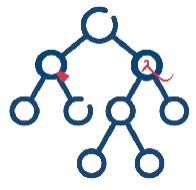
\includegraphics[height=1.0cm]{msca_logo.png}}%
    \end{center}

    \vspace{0.6cm}

    % Main title with Q logos on sides (with clickable links)
    \begin{center}
        \begin{minipage}{0.1\textwidth}
            \centering
            \href{https://quantlet.com}{
\includegraphics[height=1.1cm]{ql_logo.png}}
        \end{minipage}%
        \begin{minipage}{0.78\textwidth}
            \centering
            {\LARGE\bfseries\usebeamercolor[fg]{title}\inserttitle}

            \vspace{0.3cm}

            {\usebeamerfont{subtitle}\usebeamercolor[fg]{title}\insertsubtitle}
        \end{minipage}%
        \begin{minipage}{0.1\textwidth}
            \centering
            \href{https://quantinar.com}{
\includegraphics[height=1.1cm]{qr_logo.png}}
        \end{minipage}
    \end{center}

    \vspace{0.6cm}

    % Authors (left aligned)
    \hspace{0.5cm}{\usebeamerfont{author}\insertauthor}

    \vspace{0.3cm}

    % Institute/Affiliations (left aligned)
    \hspace{0.5cm}\begin{minipage}[t]{0.9\textwidth}
        \raggedright\small\insertinstitute
    \end{minipage}
}

%=============================================================================
% THEOREM ENVIRONMENTS
%=============================================================================
\theoremstyle{definition}
\setbeamertemplate{theorems}[numbered]
\ifdefined\atslang
\newtheorem{defn}{Definiție}
\newtheorem{thm}{Teoremă}
\newtheorem{prop}{Propoziție}
\newtheorem{rmk}{Observație}
\else
\newtheorem{defn}{Definition}
\newtheorem{thm}{Theorem}
\newtheorem{prop}{Proposition}
\newtheorem{rmk}{Remark}
\fi

%=============================================================================
% CENTRED MINIPAGE (no extra vertical space)
%=============================================================================
\newenvironment{cminipage}[1]{%
    \par\noindent\hfill\begin{minipage}{#1}\ignorespaces
}{%
    \end{minipage}\hfill\null\par
}

%=============================================================================
% CUSTOM COMMANDS
%=============================================================================
\newcommand{\E}{\mathbb{E}}
\newcommand{\Var}{\text{Var}}
\newcommand{\Cov}{\text{Cov}}
\newcommand{\Corr}{\text{Corr}}
\newcommand{\R}{\mathbb{R}}
\newcommand{\N}{\mathbb{N}}
\newcommand{\Z}{\mathbb{Z}}
\newcommand{\B}{\mathbf{B}}
\newcommand{\imark}{\textcolor{MainBlue}{\textbullet}}
\newcommand{\RMSE}{\text{RMSE}}
\newcommand{\MAE}{\text{MAE}}
\newcommand{\MAPE}{\text{MAPE}}

% Boldface vector/matrix commands (VAR, VECM, state space)
\newcommand{\bY}{\mathbf{Y}}
\newcommand{\bX}{\mathbf{X}}
\newcommand{\bA}{\mathbf{A}}
\newcommand{\bB}{\mathbf{B}}
\newcommand{\bepsilon}{\boldsymbol{\varepsilon}}
\newcommand{\bSigma}{\boldsymbol{\Sigma}}
\newcommand{\bPhi}{\boldsymbol{\Phi}}
\newcommand{\bGamma}{\boldsymbol{\Gamma}}
\newcommand{\bPi}{\boldsymbol{\Pi}}
\newcommand{\bc}{\mathbf{c}}
\newcommand{\balpha}{\boldsymbol{\alpha}}
\newcommand{\bbeta}{\boldsymbol{\beta}}
\newcommand{\bvarepsilon}{\boldsymbol{\varepsilon}}

% Seminar marks
\newcommand{\correct}{\textcolor{Forest}{\checkmark}}
\newcommand{\incorrect}{\textcolor{Crimson}{\texttimes}}
 se definește
%   \newcommand{\coursename}{Advanced Time Series Analysis and Forecasting}          (EN)
%   \newcommand{\coursename}{Analiza avansată a seriilor de timp și previziune}       (RO)  și  \def\atslang{ro}
% Fișierele .tex se află în EN/Courses, EN/Seminars, RO/Cursuri, RO/Seminarii (două niveluri sub rădăcină).
% Deck-urile sînt generate de latex/build_chapterN.py / build_seminarN.py (vezi latex/ats_build.py).

\documentclass[9pt, aspectratio=169, t]{beamer}
\providecommand{\coursename}{Advanced Time Series Analysis and Forecasting}

% Ensure content fits on slides
\setbeamersize{text margin left=8mm, text margin right=8mm}
% Smaller institute font (title page)
\setbeamerfont{institute}{size=\footnotesize}

%=============================================================================
% THEME AND STYLE CONFIGURATION
%=============================================================================
\usetheme{default}
% Using default theme for clean header/footer control

% Color Palette (matching Redispatch PDF)
\definecolor{MainBlue}{RGB}{26, 58, 110}
\definecolor{AccentBlue}{RGB}{26, 58, 110}
\definecolor{IDAred}{RGB}{205, 0, 0}
\definecolor{DarkGray}{RGB}{51, 51, 51}
\definecolor{MediumGray}{RGB}{128, 128, 128}
\definecolor{LightGray}{RGB}{248, 248, 248}
\definecolor{VeryLightGray}{RGB}{235, 235, 235}
\definecolor{KeynoteGray}{RGB}{218, 218, 218}
\definecolor{SectionGray}{RGB}{120, 120, 120}
\definecolor{FooterGray}{RGB}{100, 100, 100}
\definecolor{Crimson}{RGB}{220, 53, 69}
\definecolor{Forest}{RGB}{46, 125, 50}
\definecolor{Amber}{RGB}{181, 133, 63}
\definecolor{Orange}{RGB}{230, 126, 34}
\definecolor{Purple}{RGB}{142, 68, 173}

% Gradient background (exact Keynote 315° gradient: white to RGB 218,218,218)
\setbeamertemplate{background}{%
    \begin{tikzpicture}[remember picture, overlay]
        \shade[shading=axis, shading angle=315,
        top color=white, bottom color=KeynoteGray]
        (current page.south west) rectangle (current page.north east);
    \end{tikzpicture}%
}
% Fallback solid color for compatibility
\setbeamercolor{background canvas}{bg=}

\setbeamercolor{palette primary}{bg=MainBlue, fg=white}
\setbeamercolor{palette secondary}{bg=MainBlue!85, fg=white}
\setbeamercolor{palette tertiary}{bg=MainBlue!70, fg=white}
\setbeamercolor{structure}{fg=MainBlue}
\setbeamercolor{title}{fg=IDAred}
\setbeamercolor{frametitle}{fg=IDAred, bg=}
\setbeamercolor{block title}{bg=MainBlue, fg=white}
\setbeamercolor{block body}{bg=VeryLightGray, fg=DarkGray}
\setbeamercolor{block title alerted}{bg=Crimson, fg=white}
\setbeamercolor{block body alerted}{bg=Crimson!8, fg=DarkGray}
\setbeamercolor{block title example}{bg=Forest, fg=white}
\setbeamercolor{block body example}{bg=Forest!8, fg=DarkGray}
\setbeamercolor{item}{fg=MainBlue}

% Footer colors (override Madrid theme blue)
\setbeamercolor{author in head/foot}{fg=FooterGray, bg=}
\setbeamercolor{title in head/foot}{fg=FooterGray, bg=}
\setbeamercolor{date in head/foot}{fg=FooterGray, bg=}
\setbeamercolor{section in head/foot}{fg=FooterGray, bg=}
\setbeamercolor{subsection in head/foot}{fg=FooterGray, bg=}

% Bullet styles (apply everywhere including blocks)
\setbeamertemplate{itemize item}{\color{MainBlue}$\boxdot$}
\setbeamertemplate{itemize subitem}{\color{MainBlue}$\blacktriangleright$}
\setbeamertemplate{itemize subsubitem}{\color{MainBlue}\tiny$\bullet$}
\setbeamertemplate{itemize/enumerate body begin}{\normalsize}
\setbeamertemplate{itemize/enumerate subbody begin}{\normalsize}

% Item spacing - compact style
\setlength{\leftmargini}{10pt}       % Level 1: minimal indent
\setlength{\leftmarginii}{10pt}      % Level 2: minimal additional indent
% Compact list spacing (zero extra space before/after lists in blocks)
\makeatletter
\def\@listi{\leftmargin\leftmargini \topsep 0pt \parsep 0pt \itemsep 0pt}
\def\@listii{\leftmargin\leftmarginii \topsep 0pt \parsep 0pt \itemsep 0pt}
\makeatother

\setbeamertemplate{navigation symbols}{}

%=============================================================================
% CUSTOM HEADLINE
%=============================================================================
\setbeamertemplate{headline}{%
    \vskip10pt%
    \hbox to \paperwidth{%
        \hskip0.5cm%
        {\small\color{FooterGray}\renewcommand{\hyperlink}[2]{##2}\insertsectionhead}%
        \hfill%
        \textcolor{FooterGray}{\small\insertframenumber}%
        \hskip0.5cm%
    }%
    \vskip4pt%
    {\color{FooterGray}\hrule height 0.4pt}%
}

%=============================================================================
% CUSTOM FOOTER
%=============================================================================
\usepackage{fontawesome5}

\setbeamertemplate{footline}{%
    {\color{FooterGray}\hrule height 0.4pt}%
    \vskip4pt%
    \hbox to \paperwidth{%
        \hskip0.5cm%
        \textcolor{FooterGray}{\small\coursename}%
        \hfill%
        \raisebox{-0.1em}{%
            \begin{tikzpicture}[x=0.08em, y=0.08em, line width=0.4pt]
                \draw[FooterGray] (0,3) -- (1,4) -- (2,3.5) -- (3,5) -- (4,4) -- (5,6) -- (6,5.5) -- (7,4) -- (8,5) -- (9,7) -- (10,6) -- (11,5) -- (12,6.5) -- (13,8) -- (14,7) -- (15,6) -- (16,7.5) -- (17,9) -- (18,8) -- (19,7) -- (20,8.5) -- (21,10) -- (22,9) -- (23,8) -- (24,9.5);
            \end{tikzpicture}%
        }%
        \hskip0.5cm%
    }%
    \vskip6pt%
}

%=============================================================================
% PACKAGES
%=============================================================================
\usepackage[utf8]{inputenc}
\DeclareUnicodeCharacter{03B1}{\ensuremath{\alpha}}
\usepackage[T1]{fontenc}
\usepackage{amsmath, amssymb, amsthm}
\usepackage{mathtools}
\usepackage{bm}
\usepackage{tikz}
\usetikzlibrary{arrows.meta, positioning, shapes, calc, decorations.pathreplacing, shadings}
\usepackage{booktabs}
\usepackage{multirow}
\usepackage{array}
\usepackage{graphicx}
\usepackage{animate}
\usepackage{hyperref}
\usepackage{colortbl}
\usepackage{listings}
\lstset{language=Python, basicstyle=\ttfamily\scriptsize, keywordstyle=\color{MainBlue}\bfseries,
  commentstyle=\color{Forest}, stringstyle=\color{Crimson}, breaklines=true,
  frame=none, backgroundcolor=\color{VeryLightGray}, xleftmargin=2mm}
\hypersetup{colorlinks=true, linkcolor=MainBlue, urlcolor=MainBlue}
\graphicspath{{../../logos/}{../../charts/}{../../photos/}}
\usepackage{xcolor}
\hfuzz=2pt  % Suppress tiny overfull warnings (<2pt)
\vfuzz=2pt  % Suppress tiny vertical overfull warnings (<2pt)

%=============================================================================
% QUANTLET COMMANDS
%   \quantlet{<displayed name>}{<url>}       (generic)
%   \atsquantlet{Ch_05}{ATS_ch5_garch}       -> https://github.com/danpele/Advanced-Time-Series/tree/main/Quantlets/Ch_05/ATS_ch5_garch
%   \qlurl{<folder>} is defined per chapter by the generator (Quantlets/Ch_NN/<folder>)
%=============================================================================
\newcommand{\atsrepo}{https://github.com/danpele/Advanced-Time-Series}
\newcommand{\atsqlbase}{https://github.com/danpele/Advanced-Time-Series/tree/main/Quantlets}
\newcommand{\quantlet}[2]{%
    \hfill\href{#2}{%
        \raisebox{-0.15em}{
\includegraphics[height=0.7em]{ql_logo.png}}%
        \textcolor{MainBlue}{\tiny\ #1}%
    }%
}
\newcommand{\atsquantlet}[2]{\quantlet{\detokenize{#2}}{\atsqlbase/#1/#2}}

%=============================================================================
% NOTEBOOKS (Google Colab)
%   \colaburl{notebooks/EN/chapter5_seminar_notebook.ipynb} -> the Colab link of a file in the ATS repo
%   \nb: the chapter notebook (each seminar deck redefines it with \renewcommand)
%=============================================================================
\newcommand{\colaburl}[1]{https://colab.research.google.com/github/danpele/Advanced-Time-Series/blob/main/#1}
\newcommand{\nb}{https://colab.research.google.com/github/danpele/Advanced-Time-Series/tree/main/notebooks/EN}
\newcommand{\nbname}{notebooks/EN}

%=============================================================================
% SLIDE HELPERS (used by the generators; the same as in MFM)
%=============================================================================
% local font size for list bodies (the preamble forces \normalsize)
\newcommand{\itemsize}[1]{\setbeamertemplate{itemize/enumerate body begin}{#1}\setbeamertemplate{itemize/enumerate subbody begin}{#1}}
\newcommand{\intitle}[1]{{\hypersetup{urlcolor=white}#1}}   % white links inside coloured title bars
\newcommand{\imgcap}[1]{{\scriptsize #1}\\[0.5mm]}          % caption under a photo
\newcommand{\imgcredit}[2]{{\tiny\color{FooterGray}\href{#1}{#2}}}   % image credit: source URL, author/licence
\newcommand{\aiprompt}[1]{{\ttfamily\color{MainBlue}#1}}     % a prompt to an AI assistant

%=============================================================================
% SEMINARS: student version by default; the instructor wrapper *_solutions.tex sets \solutionstrue
%=============================================================================
\makeatletter\@ifundefined{ifsolutions}{\expandafter\newif\csname ifsolutions\endcsname}{}\makeatother
\newcommand{\solonly}[1]{\ifsolutions #1\fi}
\newcommand{\propsub}{\ifsolutions\else\framesubtitle{\ifdefined\atslang Rezolvarea se discută la seminar\else Solution discussed in class\fi}\fi}

%=============================================================================
% APPENDIX AND CHAPTER LINKS (latex/appendix_links.py writes the calls; it also re-declares these
% macros before \begin{document}, so the decks compile with or without this preamble block)
%=============================================================================
\providecommand{\atsapplink}[3]{\hypertarget{#2}{}\hyperlink{#1}{\beamergotobutton{#3}}}
\providecommand{\atsappback}[2]{\begin{tikzpicture}[remember picture,overlay]\node[anchor=south east] at ([xshift=-3mm,yshift=7mm]current page.south east){\hyperlink{#1}{\beamerreturnbutton{#2}}};\end{tikzpicture}}
\providecommand{\atschlink}[2]{\href{#1}{#2}}
\providecommand{\atschlinkt}[2]{\href{#1}{\usebeamercolor[fg]{frametitle}#2}}

%=============================================================================
% QUANTINAR COMMAND: link către un curs Quantinar (subiecte avansate)
%=============================================================================
\newcommand{\quantinar}[2]{%
    \href{#2}{%
        \raisebox{-0.15em}{
\includegraphics[height=0.8em]{qr_logo.png}}%
        \textcolor{MainBlue}{\scriptsize\ #1}%
    }%
}

%=============================================================================
% CUSTOM TITLE PAGE
%=============================================================================
\defbeamertemplate*{title page}{hybrid}[1][]
{
    \vspace{0.2cm}
    % Logos row - top header (with clickable links)
    \begin{center}
        \href{https://www.ase.ro}{
\includegraphics[height=1.0cm]{ase_logo.png}}\hspace{0.3cm}%
        \href{https://theida.net}{
\includegraphics[height=1.0cm]{ida_logo.png}}\hspace{0.3cm}%
        \href{https://blockchain-research-center.com}{
\includegraphics[height=1.0cm]{brc_logo.png}}\hspace{0.3cm}%
        \href{https://www.ai4efin.ase.ro}{
\includegraphics[height=1.0cm]{ai4efin_logo.png}}\hspace{0.3cm}%
        \href{https://ipe.ro/new}{
\includegraphics[height=1.0cm]{acad_logo.png}}\hspace{0.3cm}%
        \href{https://www.digital-finance-msca.com}{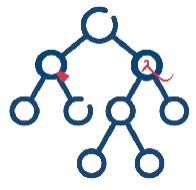
\includegraphics[height=1.0cm]{msca_logo.png}}%
    \end{center}

    \vspace{0.6cm}

    % Main title with Q logos on sides (with clickable links)
    \begin{center}
        \begin{minipage}{0.1\textwidth}
            \centering
            \href{https://quantlet.com}{
\includegraphics[height=1.1cm]{ql_logo.png}}
        \end{minipage}%
        \begin{minipage}{0.78\textwidth}
            \centering
            {\LARGE\bfseries\usebeamercolor[fg]{title}\inserttitle}

            \vspace{0.3cm}

            {\usebeamerfont{subtitle}\usebeamercolor[fg]{title}\insertsubtitle}
        \end{minipage}%
        \begin{minipage}{0.1\textwidth}
            \centering
            \href{https://quantinar.com}{
\includegraphics[height=1.1cm]{qr_logo.png}}
        \end{minipage}
    \end{center}

    \vspace{0.6cm}

    % Authors (left aligned)
    \hspace{0.5cm}{\usebeamerfont{author}\insertauthor}

    \vspace{0.3cm}

    % Institute/Affiliations (left aligned)
    \hspace{0.5cm}\begin{minipage}[t]{0.9\textwidth}
        \raggedright\small\insertinstitute
    \end{minipage}
}

%=============================================================================
% THEOREM ENVIRONMENTS
%=============================================================================
\theoremstyle{definition}
\setbeamertemplate{theorems}[numbered]
\ifdefined\atslang
\newtheorem{defn}{Definiție}
\newtheorem{thm}{Teoremă}
\newtheorem{prop}{Propoziție}
\newtheorem{rmk}{Observație}
\else
\newtheorem{defn}{Definition}
\newtheorem{thm}{Theorem}
\newtheorem{prop}{Proposition}
\newtheorem{rmk}{Remark}
\fi

%=============================================================================
% CENTRED MINIPAGE (no extra vertical space)
%=============================================================================
\newenvironment{cminipage}[1]{%
    \par\noindent\hfill\begin{minipage}{#1}\ignorespaces
}{%
    \end{minipage}\hfill\null\par
}

%=============================================================================
% CUSTOM COMMANDS
%=============================================================================
\newcommand{\E}{\mathbb{E}}
\newcommand{\Var}{\text{Var}}
\newcommand{\Cov}{\text{Cov}}
\newcommand{\Corr}{\text{Corr}}
\newcommand{\R}{\mathbb{R}}
\newcommand{\N}{\mathbb{N}}
\newcommand{\Z}{\mathbb{Z}}
\newcommand{\B}{\mathbf{B}}
\newcommand{\imark}{\textcolor{MainBlue}{\textbullet}}
\newcommand{\RMSE}{\text{RMSE}}
\newcommand{\MAE}{\text{MAE}}
\newcommand{\MAPE}{\text{MAPE}}

% Boldface vector/matrix commands (VAR, VECM, state space)
\newcommand{\bY}{\mathbf{Y}}
\newcommand{\bX}{\mathbf{X}}
\newcommand{\bA}{\mathbf{A}}
\newcommand{\bB}{\mathbf{B}}
\newcommand{\bepsilon}{\boldsymbol{\varepsilon}}
\newcommand{\bSigma}{\boldsymbol{\Sigma}}
\newcommand{\bPhi}{\boldsymbol{\Phi}}
\newcommand{\bGamma}{\boldsymbol{\Gamma}}
\newcommand{\bPi}{\boldsymbol{\Pi}}
\newcommand{\bc}{\mathbf{c}}
\newcommand{\balpha}{\boldsymbol{\alpha}}
\newcommand{\bbeta}{\boldsymbol{\beta}}
\newcommand{\bvarepsilon}{\boldsymbol{\varepsilon}}

% Seminar marks
\newcommand{\correct}{\textcolor{Forest}{\checkmark}}
\newcommand{\incorrect}{\textcolor{Crimson}{\texttimes}}
 se definește
%   \newcommand{\coursename}{Advanced Time Series Analysis and Forecasting}          (EN)
%   \newcommand{\coursename}{Analiza avansată a seriilor de timp și previziune}       (RO)  și  \def\atslang{ro}
% Fișierele .tex se află în EN/Courses, EN/Seminars, RO/Cursuri, RO/Seminarii (două niveluri sub rădăcină).
% Deck-urile sînt generate de latex/build_chapterN.py / build_seminarN.py (vezi latex/ats_build.py).

\documentclass[9pt, aspectratio=169, t]{beamer}
\providecommand{\coursename}{Advanced Time Series Analysis and Forecasting}

% Ensure content fits on slides
\setbeamersize{text margin left=8mm, text margin right=8mm}
% Smaller institute font (title page)
\setbeamerfont{institute}{size=\footnotesize}

%=============================================================================
% THEME AND STYLE CONFIGURATION
%=============================================================================
\usetheme{default}
% Using default theme for clean header/footer control

% Color Palette (matching Redispatch PDF)
\definecolor{MainBlue}{RGB}{26, 58, 110}
\definecolor{AccentBlue}{RGB}{26, 58, 110}
\definecolor{IDAred}{RGB}{205, 0, 0}
\definecolor{DarkGray}{RGB}{51, 51, 51}
\definecolor{MediumGray}{RGB}{128, 128, 128}
\definecolor{LightGray}{RGB}{248, 248, 248}
\definecolor{VeryLightGray}{RGB}{235, 235, 235}
\definecolor{KeynoteGray}{RGB}{218, 218, 218}
\definecolor{SectionGray}{RGB}{120, 120, 120}
\definecolor{FooterGray}{RGB}{100, 100, 100}
\definecolor{Crimson}{RGB}{220, 53, 69}
\definecolor{Forest}{RGB}{46, 125, 50}
\definecolor{Amber}{RGB}{181, 133, 63}
\definecolor{Orange}{RGB}{230, 126, 34}
\definecolor{Purple}{RGB}{142, 68, 173}

% Gradient background (exact Keynote 315° gradient: white to RGB 218,218,218)
\setbeamertemplate{background}{%
    \begin{tikzpicture}[remember picture, overlay]
        \shade[shading=axis, shading angle=315,
        top color=white, bottom color=KeynoteGray]
        (current page.south west) rectangle (current page.north east);
    \end{tikzpicture}%
}
% Fallback solid color for compatibility
\setbeamercolor{background canvas}{bg=}

\setbeamercolor{palette primary}{bg=MainBlue, fg=white}
\setbeamercolor{palette secondary}{bg=MainBlue!85, fg=white}
\setbeamercolor{palette tertiary}{bg=MainBlue!70, fg=white}
\setbeamercolor{structure}{fg=MainBlue}
\setbeamercolor{title}{fg=IDAred}
\setbeamercolor{frametitle}{fg=IDAred, bg=}
\setbeamercolor{block title}{bg=MainBlue, fg=white}
\setbeamercolor{block body}{bg=VeryLightGray, fg=DarkGray}
\setbeamercolor{block title alerted}{bg=Crimson, fg=white}
\setbeamercolor{block body alerted}{bg=Crimson!8, fg=DarkGray}
\setbeamercolor{block title example}{bg=Forest, fg=white}
\setbeamercolor{block body example}{bg=Forest!8, fg=DarkGray}
\setbeamercolor{item}{fg=MainBlue}

% Footer colors (override Madrid theme blue)
\setbeamercolor{author in head/foot}{fg=FooterGray, bg=}
\setbeamercolor{title in head/foot}{fg=FooterGray, bg=}
\setbeamercolor{date in head/foot}{fg=FooterGray, bg=}
\setbeamercolor{section in head/foot}{fg=FooterGray, bg=}
\setbeamercolor{subsection in head/foot}{fg=FooterGray, bg=}

% Bullet styles (apply everywhere including blocks)
\setbeamertemplate{itemize item}{\color{MainBlue}$\boxdot$}
\setbeamertemplate{itemize subitem}{\color{MainBlue}$\blacktriangleright$}
\setbeamertemplate{itemize subsubitem}{\color{MainBlue}\tiny$\bullet$}
\setbeamertemplate{itemize/enumerate body begin}{\normalsize}
\setbeamertemplate{itemize/enumerate subbody begin}{\normalsize}

% Item spacing - compact style
\setlength{\leftmargini}{10pt}       % Level 1: minimal indent
\setlength{\leftmarginii}{10pt}      % Level 2: minimal additional indent
% Compact list spacing (zero extra space before/after lists in blocks)
\makeatletter
\def\@listi{\leftmargin\leftmargini \topsep 0pt \parsep 0pt \itemsep 0pt}
\def\@listii{\leftmargin\leftmarginii \topsep 0pt \parsep 0pt \itemsep 0pt}
\makeatother

\setbeamertemplate{navigation symbols}{}

%=============================================================================
% CUSTOM HEADLINE
%=============================================================================
\setbeamertemplate{headline}{%
    \vskip10pt%
    \hbox to \paperwidth{%
        \hskip0.5cm%
        {\small\color{FooterGray}\renewcommand{\hyperlink}[2]{##2}\insertsectionhead}%
        \hfill%
        \textcolor{FooterGray}{\small\insertframenumber}%
        \hskip0.5cm%
    }%
    \vskip4pt%
    {\color{FooterGray}\hrule height 0.4pt}%
}

%=============================================================================
% CUSTOM FOOTER
%=============================================================================
\usepackage{fontawesome5}

\setbeamertemplate{footline}{%
    {\color{FooterGray}\hrule height 0.4pt}%
    \vskip4pt%
    \hbox to \paperwidth{%
        \hskip0.5cm%
        \textcolor{FooterGray}{\small\coursename}%
        \hfill%
        \raisebox{-0.1em}{%
            \begin{tikzpicture}[x=0.08em, y=0.08em, line width=0.4pt]
                \draw[FooterGray] (0,3) -- (1,4) -- (2,3.5) -- (3,5) -- (4,4) -- (5,6) -- (6,5.5) -- (7,4) -- (8,5) -- (9,7) -- (10,6) -- (11,5) -- (12,6.5) -- (13,8) -- (14,7) -- (15,6) -- (16,7.5) -- (17,9) -- (18,8) -- (19,7) -- (20,8.5) -- (21,10) -- (22,9) -- (23,8) -- (24,9.5);
            \end{tikzpicture}%
        }%
        \hskip0.5cm%
    }%
    \vskip6pt%
}

%=============================================================================
% PACKAGES
%=============================================================================
\usepackage[utf8]{inputenc}
\DeclareUnicodeCharacter{03B1}{\ensuremath{\alpha}}
\usepackage[T1]{fontenc}
\usepackage{amsmath, amssymb, amsthm}
\usepackage{mathtools}
\usepackage{bm}
\usepackage{tikz}
\usetikzlibrary{arrows.meta, positioning, shapes, calc, decorations.pathreplacing, shadings}
\usepackage{booktabs}
\usepackage{multirow}
\usepackage{array}
\usepackage{graphicx}
\usepackage{animate}
\usepackage{hyperref}
\usepackage{colortbl}
\usepackage{listings}
\lstset{language=Python, basicstyle=\ttfamily\scriptsize, keywordstyle=\color{MainBlue}\bfseries,
  commentstyle=\color{Forest}, stringstyle=\color{Crimson}, breaklines=true,
  frame=none, backgroundcolor=\color{VeryLightGray}, xleftmargin=2mm}
\hypersetup{colorlinks=true, linkcolor=MainBlue, urlcolor=MainBlue}
\graphicspath{{../../logos/}{../../charts/}{../../photos/}}
\usepackage{xcolor}
\hfuzz=2pt  % Suppress tiny overfull warnings (<2pt)
\vfuzz=2pt  % Suppress tiny vertical overfull warnings (<2pt)

%=============================================================================
% QUANTLET COMMANDS
%   \quantlet{<displayed name>}{<url>}       (generic)
%   \atsquantlet{Ch_05}{ATS_ch5_garch}       -> https://github.com/danpele/Advanced-Time-Series/tree/main/Quantlets/Ch_05/ATS_ch5_garch
%   \qlurl{<folder>} is defined per chapter by the generator (Quantlets/Ch_NN/<folder>)
%=============================================================================
\newcommand{\atsrepo}{https://github.com/danpele/Advanced-Time-Series}
\newcommand{\atsqlbase}{https://github.com/danpele/Advanced-Time-Series/tree/main/Quantlets}
\newcommand{\quantlet}[2]{%
    \hfill\href{#2}{%
        \raisebox{-0.15em}{
\includegraphics[height=0.7em]{ql_logo.png}}%
        \textcolor{MainBlue}{\tiny\ #1}%
    }%
}
\newcommand{\atsquantlet}[2]{\quantlet{\detokenize{#2}}{\atsqlbase/#1/#2}}

%=============================================================================
% NOTEBOOKS (Google Colab)
%   \colaburl{notebooks/EN/chapter5_seminar_notebook.ipynb} -> the Colab link of a file in the ATS repo
%   \nb: the chapter notebook (each seminar deck redefines it with \renewcommand)
%=============================================================================
\newcommand{\colaburl}[1]{https://colab.research.google.com/github/danpele/Advanced-Time-Series/blob/main/#1}
\newcommand{\nb}{https://colab.research.google.com/github/danpele/Advanced-Time-Series/tree/main/notebooks/EN}
\newcommand{\nbname}{notebooks/EN}

%=============================================================================
% SLIDE HELPERS (used by the generators; the same as in MFM)
%=============================================================================
% local font size for list bodies (the preamble forces \normalsize)
\newcommand{\itemsize}[1]{\setbeamertemplate{itemize/enumerate body begin}{#1}\setbeamertemplate{itemize/enumerate subbody begin}{#1}}
\newcommand{\intitle}[1]{{\hypersetup{urlcolor=white}#1}}   % white links inside coloured title bars
\newcommand{\imgcap}[1]{{\scriptsize #1}\\[0.5mm]}          % caption under a photo
\newcommand{\imgcredit}[2]{{\tiny\color{FooterGray}\href{#1}{#2}}}   % image credit: source URL, author/licence
\newcommand{\aiprompt}[1]{{\ttfamily\color{MainBlue}#1}}     % a prompt to an AI assistant

%=============================================================================
% SEMINARS: student version by default; the instructor wrapper *_solutions.tex sets \solutionstrue
%=============================================================================
\makeatletter\@ifundefined{ifsolutions}{\expandafter\newif\csname ifsolutions\endcsname}{}\makeatother
\newcommand{\solonly}[1]{\ifsolutions #1\fi}
\newcommand{\propsub}{\ifsolutions\else\framesubtitle{\ifdefined\atslang Rezolvarea se discută la seminar\else Solution discussed in class\fi}\fi}

%=============================================================================
% APPENDIX AND CHAPTER LINKS (latex/appendix_links.py writes the calls; it also re-declares these
% macros before \begin{document}, so the decks compile with or without this preamble block)
%=============================================================================
\providecommand{\atsapplink}[3]{\hypertarget{#2}{}\hyperlink{#1}{\beamergotobutton{#3}}}
\providecommand{\atsappback}[2]{\begin{tikzpicture}[remember picture,overlay]\node[anchor=south east] at ([xshift=-3mm,yshift=7mm]current page.south east){\hyperlink{#1}{\beamerreturnbutton{#2}}};\end{tikzpicture}}
\providecommand{\atschlink}[2]{\href{#1}{#2}}
\providecommand{\atschlinkt}[2]{\href{#1}{\usebeamercolor[fg]{frametitle}#2}}

%=============================================================================
% QUANTINAR COMMAND: link către un curs Quantinar (subiecte avansate)
%=============================================================================
\newcommand{\quantinar}[2]{%
    \href{#2}{%
        \raisebox{-0.15em}{
\includegraphics[height=0.8em]{qr_logo.png}}%
        \textcolor{MainBlue}{\scriptsize\ #1}%
    }%
}

%=============================================================================
% CUSTOM TITLE PAGE
%=============================================================================
\defbeamertemplate*{title page}{hybrid}[1][]
{
    \vspace{0.2cm}
    % Logos row - top header (with clickable links)
    \begin{center}
        \href{https://www.ase.ro}{
\includegraphics[height=1.0cm]{ase_logo.png}}\hspace{0.3cm}%
        \href{https://theida.net}{
\includegraphics[height=1.0cm]{ida_logo.png}}\hspace{0.3cm}%
        \href{https://blockchain-research-center.com}{
\includegraphics[height=1.0cm]{brc_logo.png}}\hspace{0.3cm}%
        \href{https://www.ai4efin.ase.ro}{
\includegraphics[height=1.0cm]{ai4efin_logo.png}}\hspace{0.3cm}%
        \href{https://ipe.ro/new}{
\includegraphics[height=1.0cm]{acad_logo.png}}\hspace{0.3cm}%
        \href{https://www.digital-finance-msca.com}{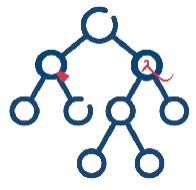
\includegraphics[height=1.0cm]{msca_logo.png}}%
    \end{center}

    \vspace{0.6cm}

    % Main title with Q logos on sides (with clickable links)
    \begin{center}
        \begin{minipage}{0.1\textwidth}
            \centering
            \href{https://quantlet.com}{
\includegraphics[height=1.1cm]{ql_logo.png}}
        \end{minipage}%
        \begin{minipage}{0.78\textwidth}
            \centering
            {\LARGE\bfseries\usebeamercolor[fg]{title}\inserttitle}

            \vspace{0.3cm}

            {\usebeamerfont{subtitle}\usebeamercolor[fg]{title}\insertsubtitle}
        \end{minipage}%
        \begin{minipage}{0.1\textwidth}
            \centering
            \href{https://quantinar.com}{
\includegraphics[height=1.1cm]{qr_logo.png}}
        \end{minipage}
    \end{center}

    \vspace{0.6cm}

    % Authors (left aligned)
    \hspace{0.5cm}{\usebeamerfont{author}\insertauthor}

    \vspace{0.3cm}

    % Institute/Affiliations (left aligned)
    \hspace{0.5cm}\begin{minipage}[t]{0.9\textwidth}
        \raggedright\small\insertinstitute
    \end{minipage}
}

%=============================================================================
% THEOREM ENVIRONMENTS
%=============================================================================
\theoremstyle{definition}
\setbeamertemplate{theorems}[numbered]
\ifdefined\atslang
\newtheorem{defn}{Definiție}
\newtheorem{thm}{Teoremă}
\newtheorem{prop}{Propoziție}
\newtheorem{rmk}{Observație}
\else
\newtheorem{defn}{Definition}
\newtheorem{thm}{Theorem}
\newtheorem{prop}{Proposition}
\newtheorem{rmk}{Remark}
\fi

%=============================================================================
% CENTRED MINIPAGE (no extra vertical space)
%=============================================================================
\newenvironment{cminipage}[1]{%
    \par\noindent\hfill\begin{minipage}{#1}\ignorespaces
}{%
    \end{minipage}\hfill\null\par
}

%=============================================================================
% CUSTOM COMMANDS
%=============================================================================
\newcommand{\E}{\mathbb{E}}
\newcommand{\Var}{\text{Var}}
\newcommand{\Cov}{\text{Cov}}
\newcommand{\Corr}{\text{Corr}}
\newcommand{\R}{\mathbb{R}}
\newcommand{\N}{\mathbb{N}}
\newcommand{\Z}{\mathbb{Z}}
\newcommand{\B}{\mathbf{B}}
\newcommand{\imark}{\textcolor{MainBlue}{\textbullet}}
\newcommand{\RMSE}{\text{RMSE}}
\newcommand{\MAE}{\text{MAE}}
\newcommand{\MAPE}{\text{MAPE}}

% Boldface vector/matrix commands (VAR, VECM, state space)
\newcommand{\bY}{\mathbf{Y}}
\newcommand{\bX}{\mathbf{X}}
\newcommand{\bA}{\mathbf{A}}
\newcommand{\bB}{\mathbf{B}}
\newcommand{\bepsilon}{\boldsymbol{\varepsilon}}
\newcommand{\bSigma}{\boldsymbol{\Sigma}}
\newcommand{\bPhi}{\boldsymbol{\Phi}}
\newcommand{\bGamma}{\boldsymbol{\Gamma}}
\newcommand{\bPi}{\boldsymbol{\Pi}}
\newcommand{\bc}{\mathbf{c}}
\newcommand{\balpha}{\boldsymbol{\alpha}}
\newcommand{\bbeta}{\boldsymbol{\beta}}
\newcommand{\bvarepsilon}{\boldsymbol{\varepsilon}}

% Seminar marks
\newcommand{\correct}{\textcolor{Forest}{\checkmark}}
\newcommand{\incorrect}{\textcolor{Crimson}{\texttimes}}


\newcommand{\qlurl}[1]{https://github.com/danpele/Advanced-Time-Series/tree/main/Quantlets/Ch_06/#1}

% Clickable citations (DOIs verified via Crossref)
\newcommand{\refAG}{\href{https://doi.org/10.1086/511283}{Aguiar și Gopinath (2007)}}
\newcommand{\refADH}{\href{https://doi.org/10.1111/j.1467-9868.2009.00736.x}{Andrieu, Doucet și Holenstein (2010)}}
\newcommand{\refAR}{\href{https://doi.org/10.1214/07-AOS574}{Andrieu și Roberts (2009)}}
\newcommand{\refAK}{\href{https://doi.org/10.1214/aos/1176349739}{Ansley și Kohn (1985)}}
\newcommand{\refBM}{\href{https://doi.org/10.1002/jae.2306}{Bańbura și Modugno (2014)}}
\newcommand{\refBN}{\href{https://doi.org/10.1016/0304-3932(81)90040-4}{Beveridge și Nelson (1981)}}
\newcommand{\refBol}{\href{https://doi.org/10.1016/0304-4076(86)90063-1}{Bollerslev (1986)}}
\newcommand{\refBro}{\href{https://doi.org/10.1214/14-AOAS788}{Brodersen et al.\ (2015)}}
\newcommand{\refCK}{\href{https://doi.org/10.1093/biomet/81.3.541}{Carter și Kohn (1994)}}
\newcommand{\refCJ}{\href{https://doi.org/10.1504/IJMMNO.2009.030090}{Chan și Jeliazkov (2009)}}
\newcommand{\refCP}{\href{https://doi.org/10.1007/978-3-030-47845-2}{Chopin și Papaspiliopoulos (2020)}}
\newcommand{\refCla}{\href{https://doi.org/10.2307/1884282}{Clark (1987)}}
\newcommand{\refCSa}{\href{https://doi.org/10.1086/654451}{Cogley și Sargent (2001)}}
\newcommand{\refCSb}{\href{https://doi.org/10.1016/j.red.2004.10.009}{Cogley și Sargent (2005)}}
\newcommand{\refdJa}{\href{https://doi.org/10.1214/aos/1176348139}{de Jong (1991)}}
\newcommand{\refdJS}{\href{https://doi.org/10.1093/biomet/82.2.339}{de Jong și Shephard (1995)}}
\newcommand{\refDM}{\href{https://doi.org/10.1007/978-1-4684-9393-1}{Del Moral (2004)}}
\newcommand{\refDNP}{\href{https://doi.org/10.1093/restud/rdv024}{Del Negro și Primiceri (2015)}}
\newcommand{\refDPDK}{\href{https://doi.org/10.1093/biomet/asu075}{Doucet, Pitt, Deligiannidis și Kohn (2015)}}
\newcommand{\refDGR}{\href{https://doi.org/10.1016/j.jeconom.2011.02.012}{Doz, Giannone și Reichlin (2011)}}
\newcommand{\refDKa}{\href{https://doi.org/10.1093/biomet/89.3.603}{Durbin și Koopman (2002)}}
\newcommand{\refDK}{\href{https://doi.org/10.1093/acprof:oso/9780199641178.001.0001}{Durbin și Koopman (2012)}}
\newcommand{\refFS}{\href{https://doi.org/10.1111/j.1467-9892.1994.tb00184.x}{Frühwirth-Schnatter (1994)}}
\newcommand{\refFSW}{\href{https://doi.org/10.1016/j.jeconom.2009.07.003}{Frühwirth-Schnatter și Wagner (2010)}}
\newcommand{\refGRS}{\href{https://doi.org/10.1016/j.jmoneco.2008.05.010}{Giannone, Reichlin și Small (2008)}}
\newcommand{\refGSS}{\href{https://doi.org/10.1049/ip-f-2.1993.0015}{Gordon, Salmond și Smith (1993)}}
\newcommand{\refHam}{\href{https://doi.org/10.2307/j.ctv14jx6sm}{Hamilton (1994)}}
\newcommand{\refHamB}{\href{https://doi.org/10.1162/rest_a_00706}{Hamilton (2018)}}
\newcommand{\refHar}{\href{https://doi.org/10.1017/CBO9781107049994}{Harvey (1990)}}
\newcommand{\refHJ}{\href{https://doi.org/10.1002/jae.3950080302}{Harvey și Jaeger (1993)}}
\newcommand{\refHRS}{\href{https://doi.org/10.2307/2297980}{Harvey, Ruiz și Shephard (1994)}}
\newcommand{\refJPR}{\href{https://doi.org/10.1080/07350015.1994.10524553}{Jacquier, Polson și Rossi (1994)}}
\newcommand{\refJU}{\href{https://doi.org/10.1109/JPROC.2003.823141}{Julier și Uhlmann (2004)}}
\newcommand{\refJK}{\href{https://doi.org/10.1111/ectj.12029}{Jungbacker și Koopman (2015)}}
\newcommand{\refKal}{\href{https://doi.org/10.1115/1.3662552}{Kalman (1960)}}
\newcommand{\refKMW}{\href{https://doi.org/10.1162/REST_a_00691}{Kamber, Morley și Wong (2018)}}
\newcommand{\refKN}{\href{https://doi.org/10.7551/mitpress/6444.001.0001}{Kim și Nelson (1999)}}
\newcommand{\refKSC}{\href{https://doi.org/10.1111/1467-937X.00050}{Kim, Shephard și Chib (1998)}}
\newcommand{\refKit}{\href{https://doi.org/10.1080/10618600.1996.10474692}{Kitagawa (1996)}}
\newcommand{\refKoo}{\href{https://doi.org/10.1080/01621459.1997.10473685}{Koopman (1997)}}
\newcommand{\refKD}{\href{https://doi.org/10.1111/1467-9892.00186}{Koopman și Durbin (2000)}}
\newcommand{\refMM}{\href{https://doi.org/10.1002/jae.695}{Mariano și Murasawa (2003)}}
\newcommand{\refMNZ}{\href{https://doi.org/10.1162/003465303765299765}{Morley, Nelson și Zivot (2003)}}
\newcommand{\refOCSN}{\href{https://doi.org/10.1016/j.jeconom.2006.07.008}{Omori, Chib, Shephard și Nakajima (2007)}}
\newcommand{\refOvN}{\href{https://doi.org/10.1162/003465302760556422}{Orphanides și van Norden (2002)}}
\newcommand{\refPet}{\href{https://doi.org/10.1016/j.ijforecast.2021.11.001}{Petropoulos et al.\ (2022)}}
\newcommand{\refPS}{\href{https://doi.org/10.1080/01621459.1999.10474153}{Pitt și Shephard (1999)}}
\newcommand{\refPSGK}{\href{https://doi.org/10.1016/j.jeconom.2012.06.004}{Pitt, Silva, Giordani și Kohn (2012)}}
\newcommand{\refPri}{\href{https://doi.org/10.1111/j.1467-937X.2005.00353.x}{Primiceri (2005)}}
\newcommand{\refSV}{\href{https://doi.org/10.1504/IJMMNO.2014.059942}{Scott și Varian (2014)}}
\newcommand{\refSH}{\href{https://doi.org/10.1111/j.1467-9892.1990.tb00062.x}{Shephard și Harvey (1990)}}
\newcommand{\refSS}{\href{https://doi.org/10.1111/j.1467-9892.1982.tb00349.x}{Shumway și Stoffer (1982)}}
\newcommand{\refSWa}{\href{https://doi.org/10.1080/01621459.1998.10474116}{Stock și Watson (1998)}}
\newcommand{\refSWb}{\href{https://doi.org/10.1111/j.1538-4616.2007.00014.x}{Stock și Watson (2007)}}
\newcommand{\refTay}{\href{https://doi.org/10.1111/j.1467-9965.1994.tb00057.x}{Taylor (1994)}}
\newcommand{\refWat}{\href{https://doi.org/10.1016/0304-3932(86)90054-1}{Watson (1986)}}

\title[Analiza avansată a seriilor de timp și previziune]{Analiza avansată a seriilor de timp și previziune}
\subtitle{Capitolul 6: Modele în spațiul stărilor și filtrare bayesiană}
\author[D.T. Pele]{Daniel Traian PELE}
\institute{Academia de Studii Economice din București\\
IDA Institute Digital Assets\\
Blockchain Research Center\\
AI4EFin Artificial Intelligence for Energy Finance\\
Academia Română, Institutul de Prognoză Economică\\
MSCA Digital Finance}
\date{}

%=============================================================================
\providecommand{\atsapplink}[3]{\hypertarget{#2}{}\hyperlink{#1}{\beamergotobutton{#3}}}  % APPLINKS-MACROS
\providecommand{\atsappback}[2]{\begin{tikzpicture}[remember picture,overlay]\node[anchor=south east] at ([xshift=-3mm,yshift=7mm]current page.south east){\hyperlink{#1}{\beamerreturnbutton{#2}}};\end{tikzpicture}}  % APPLINKS-MACROS
\providecommand{\atschlink}[2]{\href{#1}{#2}}  % APPLINKS-MACROS
\providecommand{\atschlinkt}[2]{\href{#1}{\usebeamercolor[fg]{frametitle}#2}}  % APPLINKS-MACROS
\begin{document}
%=============================================================================

{
\setbeamertemplate{headline}{}
\setbeamertemplate{footline}{}
\begin{frame}[noframenumbering]
    \titlepage
\end{frame}
}
% BEGIN-ACRONYMS (generat de latex/acronyms.py; nu editati manual)
\begin{frame}{Acronime folosite în acest material (1/3)}
\setbeamertemplate{itemize/enumerate body begin}{\footnotesize}
\begin{columns}[T]
\begin{column}{0.49\textwidth}
\begin{itemize}\setlength{\itemsep}{0pt}
    \item \textbf{AI}: Artificial Intelligence (inteligență artificială)
    \item \textbf{APF}: Auxiliary Particle Filter (filtrul de particule auxiliar)
    \item \textbf{AR}: AutoRegressive (model); in event studies: Abnormal Return (model autoregresiv; în studiile de eveniment: randament anormal)
    \item \textbf{ARCH}: AutoRegressive Conditional Heteroskedasticity (heteroscedasticitate condiționată autoregresivă)
    \item \textbf{ARIMA}: AutoRegressive Integrated Moving Average (model) — model autoregresiv integrat cu medie mobilă
    \item \textbf{ARMA}: AutoRegressive Moving Average (model) — model autoregresiv cu medie mobilă
    \item \textbf{BET}: Bucharest Exchange Trading (index) — indicele de referință al Bursei de Valori București
    \item \textbf{BN}: Beveridge–Nelson (decomposition) — descompunerea Beveridge–Nelson
    \item \textbf{BNR}: Banca Națională a României
\end{itemize}
\end{column}
\begin{column}{0.49\textwidth}
\begin{itemize}\setlength{\itemsep}{0pt}
    \item \textbf{BSTS}: Bayesian Structural Time Series (serii de timp structurale bayesiene)
    \item \textbf{BVAR}: Bayesian Vector AutoRegression (model vector autoregresiv bayesian)
    \item \textbf{DFM}: Dynamic Factor Model (model factorial dinamic)
    \item \textbf{DK}: Durbin–Koopman (simulation smoother, 2002) — algoritmul Durbin–Koopman (2002) de simulare a stărilor netezite
    \item \textbf{DSGE}: Dynamic Stochastic General Equilibrium (model) — model dinamic stochastic de echilibru general
    \item \textbf{EKF}: Extended Kalman Filter (filtrul Kalman extins)
    \item \textbf{EM}: Expectation–Maximisation (algorithm) — algoritmul expectație–maximizare
    \item \textbf{EODHD}: EOD Historical Data (market-data provider) — furnizor de date de piață
    \item \textbf{ETS}: Error, Trend, Seasonality (exponential smoothing state space models) — eroare, trend, sezonalitate (modele de netezire exponențială)
\end{itemize}
\end{column}
\end{columns}
\end{frame}
\begin{frame}{Acronime folosite în acest material (2/3)}
\setbeamertemplate{itemize/enumerate body begin}{\footnotesize}
\begin{columns}[T]
\begin{column}{0.49\textwidth}
\begin{itemize}\setlength{\itemsep}{0pt}
    \item \textbf{FERMIAC}: mechanical Monte Carlo device of Enrico Fermi (Los Alamos, 1947) — dispozitiv mecanic Monte Carlo al lui Enrico Fermi (Los Alamos, 1947)
    \item \textbf{FFBS}: Forward Filtering, Backward Sampling (filtrare înainte, eșantionare înapoi)
    \item \textbf{FRED}: Federal Reserve Economic Data (baza de date economice a Rezervei Federale din St. Louis)
    \item \textbf{GARCH}: Generalised AutoRegressive Conditional Heteroskedasticity (heteroscedasticitate condiționată autoregresivă generalizată)
    \item \textbf{HICP}: Harmonised Index of Consumer Prices (indicele armonizat al prețurilor de consum (IAPC))
    \item \textbf{HP}: Hodrick–Prescott (filter) — filtrul Hodrick–Prescott
    \item \textbf{IAPC}: Indicele armonizat al prețurilor de consum
    \item \textbf{IG}: inverse gamma (distribution) — distribuția gamma inversă
    \item \textbf{IMA}: Integrated Moving Average (model) — model integrat de medie mobilă
\end{itemize}
\end{column}
\begin{column}{0.49\textwidth}
\begin{itemize}\setlength{\itemsep}{0pt}
    \item \textbf{KSC}: Kim–Shephard–Chib (1998), mixture sampler for stochastic volatility (Kim–Shephard–Chib (1998), eșantionatorul cu mixtură pentru volatilitatea stochastică)
    \item \textbf{LLM}: Large Language Model (model lingvistic de mari dimensiuni)
    \item \textbf{LR}: Likelihood Ratio (test) — testul raportului de verosimilitate
    \item \textbf{MA}: Moving Average (medie mobilă)
    \item \textbf{MCMC}: Markov Chain Monte Carlo (metode Monte Carlo cu lanțuri Markov)
    \item \textbf{ML}: Machine Learning (învățare automată)
    \item \textbf{MNZ}: Morley–Nelson–Zivot (2003) — Morley–Nelson–Zivot (2003)
    \item \textbf{OLS}: Ordinary Least Squares (metoda celor mai mici pătrate)
    \item \textbf{PIB}: Produsul intern brut
\end{itemize}
\end{column}
\end{columns}
\end{frame}
\begin{frame}{Acronime folosite în acest material (3/3)}
\setbeamertemplate{itemize/enumerate body begin}{\footnotesize}
\begin{columns}[T]
\begin{column}{0.49\textwidth}
\begin{itemize}\setlength{\itemsep}{0pt}
    \item \textbf{PMMH}: Particle Marginal Metropolis–Hastings (algoritmul Metropolis–Hastings marginal cu filtru de particule)
    \item \textbf{QML}: Quasi-Maximum Likelihood (verosimilitate cvasi-maximă)
    \item \textbf{SMC}: Sequential Monte Carlo (metode Monte Carlo secvențiale)
    \item \textbf{SUA}: Statele Unite ale Americii
    \item \textbf{SV}: Stochastic Volatility (volatilitate stochastică)
    \item \textbf{TLC}: Teorema Limită Centrală
    \item \textbf{TSA}: Time Series Analysis (Serii de timp, cursul de licență)
    \item \textbf{TVA}: Taxa pe valoarea adăugată
    \item \textbf{TVP}: Time-Varying Parameter(s) — parametri variabili în timp
    \item \textbf{TVP-VAR}: Time-Varying-Parameter Vector AutoRegression (model VAR cu parametri variabili în timp)
\end{itemize}
\end{column}
\begin{column}{0.49\textwidth}
\begin{itemize}\setlength{\itemsep}{0pt}
    \item \textbf{TVP-VAR-SV}: TVP-VAR with Stochastic Volatility (model VAR cu parametri variabili în timp și volatilitate stochastică)
    \item \textbf{UC}: Unobserved Components (model) — model cu componente neobservate
    \item \textbf{UC-SV}: Unobserved Components model with Stochastic Volatility (Stock–Watson 2007) — model cu componente neobservate și volatilitate stochastică (Stock–Watson 2007)
    \item \textbf{UC-UR}: UC model with correlated trend and cycle shocks (Morley–Nelson–Zivot 2003) — model UC cu șocuri corelate ale trendului și ciclului (Morley–Nelson–Zivot 2003)
    \item \textbf{UC0}: UC model with uncorrelated trend and cycle shocks (Clark 1987) — model UC cu șocuri necorelate ale trendului și ciclului (Clark 1987)
    \item \textbf{UKF}: Unscented Kalman Filter (filtrul Kalman unscented)
    \item \textbf{VAR}: Vector AutoRegression (model vector autoregresiv)
\end{itemize}
\end{column}
\end{columns}
\end{frame}
% END-ACRONYMS

\begin{frame}{Întrebarea de azi și traseul}
\itemsize{\small}
\begin{itemize}
    \item \textbf{Întrebarea}: cum învățăm despre mărimi pe care nu le observăm niciodată (inflația de trend, output gap-ul, volatilitatea, coeficienți variabili în timp) și cît ne putem baza pe ce aflăm?
    \begin{itemize}
        \item un singur cadru: o ecuație de stare pentru mărimea ascunsă, o ecuație de măsurare pentru date și un filtru care actualizează convingerile pe măsură ce sosesc datele
    \end{itemize}
    \item \textbf{Traseul} capitolului
    \begin{itemize}
        \item modelul liniar gaussian general, inițializarea difuză exactă, verosimilitatea exactă și inferența la frontieră
        \item spațiul stărilor bayesian: simulation smoothers și eșantionare Gibbs; volatilitatea stochastică
        \item filtre neliniare: filtrul Kalman extins și unscented, filtre de particule, particle MCMC
        \item parametri variabili în timp, factori dinamici, descompuneri trend--ciclu și inflația de trend cu volatilitate stochastică
    \end{itemize}
    \item Pornim de la \atschlink{https://danpele.github.io/Time-Series-Analysis/RO/Cursuri/capitol10_spatiul_starilor_kalman_markov_switching.pdf}{TSA, Capitolul 10} (forma în spațiul stărilor, filtrul Kalman de mînă, netezirea, modelele local level și local trend, output gap-ul UC, bazele modelelor Markov switching); Seminarul 6 are loc înaintea acestui curs
\end{itemize}
\end{frame}

\begin{frame}{Rezultatele învățării}
\itemsize{\small}
\begin{itemize}
    \item Derivați filtrul și netezitorul Kalman pentru modelul liniar gaussian general, cu inițializare difuză exactă, și scrieți-le în \texttt{numpy}
    \item Maximizați verosimilitatea exactă și evaluați inferența asupra varianțelor care pot ajunge pe frontieră (pile-up, teste LR bootstrap)
    \item Eșantionați stările cu metodele Carter--Kohn, Durbin--Koopman și cu eșantionarea pe baza matricei de precizie, într-un eșantionator Gibbs; estimați volatilitatea stochastică prin mixtura KSC
    \item Aplicați filtrele Kalman extins, unscented și de particule; folosiți verosimilitatea din filtrul de particule în PMMH și alegeți numărul de particule
    \item Estimați regresii TVP, modele UC cu șocuri corelate și inflația de trend UC-SV și raportați cît de fragile sînt estimațiile componentelor latente
\end{itemize}
\end{frame}

\begin{frame}{Bibliografie, date și instrumente}
\itemsize{\small}
\begin{itemize}
    \item Bibliografia de bază: \refDK, cap.~2--9 și 11--14; \refHar; \refKN; \refHam, cap.~13; \refCP
    \begin{itemize}
        \item lucrările originale: \refKal, \refKoo, \refCK, \refDKa, \refKSC, \refGSS, \refPS, \refADH, \refPri, \refMNZ, \refSWb
    \end{itemize}
    \item Quantlet-urile Python ale capitolului: \href{https://github.com/danpele/Advanced-Time-Series/tree/main/Quantlets/Ch_06}{Quantlets/Ch\_06}
    \begin{itemize}
        \item filtrul și netezitorul Kalman cu inițializare difuză exactă, simulation smoothers, eșantionatorul Gibbs KSC, filtrele de particule bootstrap și auxiliar, PMMH și UC-SV scrise explicit în \texttt{numpy}; verificate cu \texttt{statsmodels}
    \end{itemize}
    \item Notebook-ul cursului: \href{\colaburl{notebooks/EN/chapter6_lecture_notebook.ipynb}}{deschideți în Google Colab}
\end{itemize}
\end{frame}

\begin{frame}{Datele folosite în acest capitol}
\itemsize{\footnotesize}
\begin{center}
\scriptsize
\begin{tabular}{>{\raggedright\arraybackslash}p{5.0cm}>{\raggedright\arraybackslash}p{4.4cm}>{\raggedright\arraybackslash}p{2.5cm}}
\toprule
\textbf{Seria} & \textbf{Sursa} & \textbf{Utilizare} \\
\midrule
deflatorul PIB și PIB-ul real al SUA (trimestrial) & FRED (GDPDEF, GDPC1) & verosimilitate, MNZ, UC-SV \\
S\&P 500 și BET, închideri zilnice & EODHD & volatilitate stochastică \\
IAPC pentru România și zona euro (indice lunar, 2025 = 100) & Eurostat prc\_hicp\_minr & TVP, UC-SV \\
PIB-ul real al României, ajustat sezonier și cu numărul de zile lucrătoare & Eurostat namq\_10\_gdp & output gap-ul \\
producția industrială, numărul de salariați, venitul real fără transferuri, vînzările reale ale SUA (lunar) & FRED (INDPRO, PAYEMS, W875RX1, CMRMTSPL) & DFM \\
\bottomrule
\end{tabular}
\end{center}
\begin{itemize}
    \item Toate sursele sînt publice și nu cer cont sau cheie; seriile trimestriale pînă în T2 2026, cele lunare pînă în august sau septembrie 2026, datele zilnice pînă la 18 septembrie 2026
    \item IAPC (HICP): indicele armonizat al prețurilor de consum; DFM: model cu factori dinamici
\end{itemize}
\end{frame}

\begin{frame}{De la navigația Apollo la inflația de trend}
\itemsize{\footnotesize}
\begin{columns}[T]
\begin{column}{0.36\textwidth}
\centering

\includegraphics[height=0.36\textheight]{ch6_kalman_2007.jpg}\\[1mm]
\imgcap{Rudolf E. Kálmán, 2007}
\imgcredit{https://commons.wikimedia.org/wiki/File:ETH-BIB-Kalman,_Rudolf_E._(1930-2016)-HK_04-01925.jpg}{Foto: ETH-Bibliothek Zürich, Bildarchiv (2007); CC BY-SA 4.0; Wikimedia Commons}
\end{column}
\begin{column}{0.62\textwidth}
\begin{itemize}
    \item 1960: \refKal\ dă filtrul liniar recursiv; în mai puțin de un deceniu, el ghidează misiunile Apollo
    \item 1982--1997: algoritmul EM pentru modele în spațiul stărilor \refSS; serii de timp structurale \refHar; filtrarea difuză exactă \refKoo
    \item 1993--1999: filtre de particule \refGSS, \refPS; eșantionarea Gibbs a stărilor \refCK, \refFS; volatilitate stochastică \refKSC
    \item 2002--2010: simulation smoother-ul \refDKa; TVP-VAR cu volatilitate stochastică \refPri, \refCSb; particle MCMC \refADH
    \item Astăzi: băncile centrale urmăresc inflația de trend și output gap-ul cu aceste instrumente \refSWb, \refMNZ
\end{itemize}
\end{column}
\end{columns}
\end{frame}


%=============================================================================
\section{Modelul liniar gaussian general}
%=============================================================================

\begin{frame}{De la TSA la acest capitol}
\itemsize{\small}
\begin{itemize}
    \item Cunoscut (\atschlink{https://danpele.github.io/Time-Series-Analysis/RO/Cursuri/capitol10_spatiul_starilor_kalman_markov_switching.pdf}{TSA, Capitolul 10}): forma în spațiul stărilor, filtrul Kalman pentru modelul local level de mînă, netezirea, verosimilitatea maximă prin descompunerea erorilor de predicție, filtrul HP ca netezitor, Hamilton (2018), modelele Markov switching
    \item Nou aici
    \begin{itemize}
        \item filtrul și netezitorul pentru orice model liniar gaussian, cu stări nestaționare inițializate exact (nu cu o varianță mare)
        \item inferența cînd o varianță poate fi zero; eșantionarea bayesiană a traiectoriilor întregi ale stărilor
        \item modele neliniare și negaussiene: volatilitate stochastică, filtre de particule, particle MCMC
        \item aplicații la nivel de cercetare: MNZ, UC-SV, regresii TVP, ragged edge într-un DFM
    \end{itemize}
    \item Modelele Markov switching în detaliu: \atschlink{https://danpele.github.io/Advanced-Time-Series/RO/Cursuri/capitol7_modele_schimbare_regim.pdf}{Capitolul 7}; nowcasting cu factori: \atschlink{https://danpele.github.io/Advanced-Time-Series/RO/Cursuri/capitol5_bvar_modele_factoriale_nowcasting.pdf}{Capitolul 5}
\end{itemize}
\end{frame}

\begin{frame}{Forma generală în spațiul stărilor (1/2)}
\itemsize{\small}
\begin{itemize}
    \item Două ecuații: datele sînt o funcție liniară cu zgomot a unei stări neobservate, iar starea urmează o dinamică liniară de ordinul întîi \[ y_t = Z_t\alpha_t + \varepsilon_t, \qquad \alpha_{t+1} = c_t + T_t\alpha_t + R_t\eta_t, \qquad t = 1, \dots, n \]
    \item Notațiile
    \begin{itemize}
        \item $y_t$ ($p\times 1$): observațiile; $\alpha_t$ ($m\times 1$): starea; $n$: lungimea eșantionului
        \item $Z_t$ ($p\times m$): matricea de măsurare; $T_t$ ($m\times m$): matricea de tranziție; $c_t$: un termen liber cunoscut
        \item $\varepsilon_t \sim N(0, H_t)$: zgomotul de măsurare; $\eta_t \sim N(0, Q_t)$: șocurile stării; $R_t$ ($m\times r$) alege stările care primesc șocuri
        \item $\varepsilon_t$ și $\eta_s$ sînt independente între ele și în timp
    \end{itemize}
    \item Starea inițială $\alpha_1 \sim N(a_1, P_1)$
    \begin{itemize}
        \item elementele nestaționare sau fixe necunoscute: $P_1 = \kappa P_\infty + P_*$, $\kappa \to \infty$; $P_\infty$ marchează elementele difuze, $P_*$ este covarianța celorlalte
    \end{itemize}
\end{itemize}
\end{frame}

\begin{frame}{Forma generală în spațiul stărilor (2/2)}
\itemsize{\small}
\begin{itemize}
    \item Matricele sistemului $Z_t, T_t, R_t, H_t, Q_t$ depind de parametrii $\psi$; variația în timp a lui $Z_t$ dă regresii cu coeficienți variabili în timp
    \begin{itemize}
        \item ARMA, UC, regresii TVP, DFM, VAR cu date lipsă, ETS: toate sînt cazuri particulare \refDK
    \end{itemize}
    \item Notațiile pentru estimații
    \begin{itemize}
        \item $Y_t = (y_1, \dots, y_t)$: datele pînă la $t$
        \item starea prezisă: $a_t = \E(\alpha_t | Y_{t-1})$, $P_t = \Var(\alpha_t | Y_{t-1})$; filtrată: $a_{t|t}$, $P_{t|t}$ (după $y_t$)
        \item netezită: $\hat\alpha_t = \E(\alpha_t | Y_n)$, $V_t = \Var(\alpha_t | Y_n)$ (toate datele)
    \end{itemize}
\end{itemize}
\end{frame}

\begin{frame}{Filtrul Kalman dintr-o singură lemă}
\itemsize{\small}
\begin{itemize}
    \item Lema (condiționarea vectorilor normali comuni): dacă $(x, y)$ este gaussian, $\E(x | y) = \mu_x + \Sigma_{xy}\Sigma_{yy}^{-1}(y - \mu_y)$, $\Var(x | y) = \Sigma_{xx} - \Sigma_{xy}\Sigma_{yy}^{-1}\Sigma_{yx}$
    \begin{itemize}
        \item $\mu_x$, $\mu_y$: mediile; $\Sigma_{xy} = \Cov(x, y)$, $\Sigma_{yy} = \Var(y)$: blocurile de covarianță
        \item o aplicăm pentru $x = \alpha_t$ și $y = y_t$, condiționat de $Y_{t-1}$: $v_t = y_t - Z_ta_t$ este informația nouă (eroarea de predicție)
    \end{itemize}
    \item Varianța erorii de predicție $\Var(v_t | Y_{t-1}) = F_t = Z_tP_tZ_t' + H_t$; $\Cov(\alpha_t, v_t | Y_{t-1}) = P_tZ_t'$; $v_t$ este independent de $Y_{t-1}$
    \item Actualizarea: $a_{t|t} = a_t + P_tZ_t'F_t^{-1}v_t$, $P_{t|t} = P_t - P_tZ_t'F_t^{-1}Z_tP_t$
    \item Predicția: $a_{t+1} = c_t + T_ta_{t|t}$, $P_{t+1} = T_tP_{t|t}T_t' + R_tQ_tR_t'$
    \item Fără normalitate, aceleași recursii dau cel mai bun predictor \emph{liniar} (eroare pătratică medie minimă printre funcțiile liniare de $Y_t$)
\end{itemize}
\end{frame}

\begin{frame}{Filtrul într-o singură trecere}
\itemsize{\small}
\begin{itemize}
    \item $v_t = y_t - Z_ta_t$, $\quad F_t = Z_tP_tZ_t' + H_t$, $\quad K_t = T_tP_tZ_t'F_t^{-1}$ (cîștigul Kalman), $\quad L_t = T_t - K_tZ_t$
    \item $a_{t+1} = c_t + T_ta_t + K_tv_t$, $\quad P_{t+1} = T_tP_tL_t' + R_tQ_tR_t'$
    \item Costul: $O(n(m^3 + p^3))$; cu matrice constante, $P_t$ converge către starea staționară a ecuației Riccati
    \begin{itemize}
        \item $P_t$ și $K_t$ nu depind de $y$: se pot calcula înainte de sosirea datelor
    \end{itemize}
    \item $y_t$ lipsă: punem $Z_t = 0$ (sau eliminăm rîndurile lipsă): $v_t$ și $K_t$ dispar, iar filtrul doar prezice
    \begin{itemize}
        \item frecvențele mixte și ragged edge al datelor în timp real se tratează deci fără cost suplimentar (\atschlink{https://danpele.github.io/Advanced-Time-Series/RO/Cursuri/capitol5_bvar_modele_factoriale_nowcasting.pdf}{Capitolul 5})
    \end{itemize}
    \item $y_t$ multivariat cu $H_t$ diagonală: prelucrăm cele $p$ elemente pe rînd (tratarea univariată \refKD): fără inversarea unei matrice $p\times p$
\end{itemize}
\end{frame}

\begin{frame}{Netezirea: recursii înapoi}
\itemsize{\small}
\begin{itemize}
    \item Netezitorul stărilor \refDK: $r_{t-1} = Z_t'F_t^{-1}v_t + L_t'r_t$, $\quad N_{t-1} = Z_t'F_t^{-1}Z_t + L_t'N_tL_t$, $\quad r_n = 0$, $N_n = 0$
    \item Starea netezită: $\hat\alpha_t = a_t + P_tr_{t-1}$, $\quad V_t = P_t - P_tN_{t-1}P_t$
    \begin{itemize}
        \item $r_{t-1}$: o sumă ponderată a inovațiilor de la $t$ încolo; $N_{t-1} = \Var(r_{t-1})$
        \item $\hat\alpha_t$ corectează $a_t$ cu tot ce aflăm de la momentul $t$ încolo
    \end{itemize}
    \item Netezitorul perturbațiilor: $\hat\varepsilon_t = H_t(F_t^{-1}v_t - K_t'r_t)$, $\hat\eta_t = Q_tR_t'r_t$: reziduuri auxiliare pentru valori extreme și rupturi și scorul verosimilității
    \item Derivarea folosește aceeași lemă, acum condiționînd pe $v_t, \dots, v_n$, care sînt independente (\atsapplink{atsapp1}{atssrc1}{Anexa})
\end{itemize}
\end{frame}

\begin{frame}{Inițializarea difuză (1/2)}
\itemsize{\small}
\begin{itemize}
    \item Mersurile aleatoare, trendurile și coeficienții de regresie nu au distribuție staționară: $P_1 = \kappa P_\infty + P_*$, $\kappa \to \infty$
    \begin{itemize}
        \item „big kappa” ($\kappa = 10^6$--$10^7$) este o aproximare cu două defecte: verosimilitatea conține termeni $-\frac12\ln\kappa$, iar erorile de rotunjire cresc cu $\kappa$
    \end{itemize}
    \item Filtrul difuz exact \refKoo, \refAK, \refdJa
    \begin{itemize}
        \item dezvoltăm $P_t = \kappa P_{\infty,t} + P_{*,t} + O(\kappa^{-1})$ și păstrăm ambele părți cît timp $P_{\infty,t} \ne 0$
        \item $P_{\infty,t}$ ajunge la zero după $d$ pași ($d$ = numărul elementelor difuze, dacă sînt identificate)
        \item apoi preia filtrul obișnuit
    \end{itemize}
\end{itemize}
\end{frame}

\begin{frame}{Inițializarea difuză (2/2)}
\itemsize{\footnotesize}
\begin{itemize}
    \item Recursiile difuze exacte
    \begin{itemize}
        \item $F_{\infty,t}$, $F_{*,t}$: părțile difuză și finită ale lui $F_t$; $K^{(0)}_t$, $K^{(1)}_t$: cîștigurile corespunzătoare; $L^{(0)}_t = T_t - K^{(0)}_tZ_t$, $L^{(1)}_t = -K^{(1)}_tZ_t$
        \item $y_t$ univariat, $F_{\infty,t} = Z_tP_{\infty,t}Z_t' > 0$: $K^{(0)}_t = T_tP_{\infty,t}Z_t'/F_{\infty,t}$, $K^{(1)}_t = T_t(P_{*,t}Z_t' - P_{\infty,t}Z_t'F_{*,t}/F_{\infty,t})/F_{\infty,t}$
        \item $a_{t+1} = c_t + T_ta_t + K^{(0)}_tv_t$; $P_{\infty,t+1} = T_tP_{\infty,t}L^{(0)\prime}_t$; $P_{*,t+1} = T_tP_{\infty,t}L^{(1)\prime}_t + T_tP_{*,t}L^{(0)\prime}_t + R_tQ_tR_t'$
    \end{itemize}
    \item Netezitorul are recursii difuze corespunzătoare pentru $r^{(0)}, r^{(1)}, N^{(0)}, N^{(1)}, N^{(2)}$ \refDK, secțiunea 5.3; în Quantlet ambele sînt comparate cu \texttt{statsmodels}
\end{itemize}
\end{frame}

\begin{frame}{Inițializarea difuză exactă față de big kappa}
\itemsize{\footnotesize}
\begin{center}
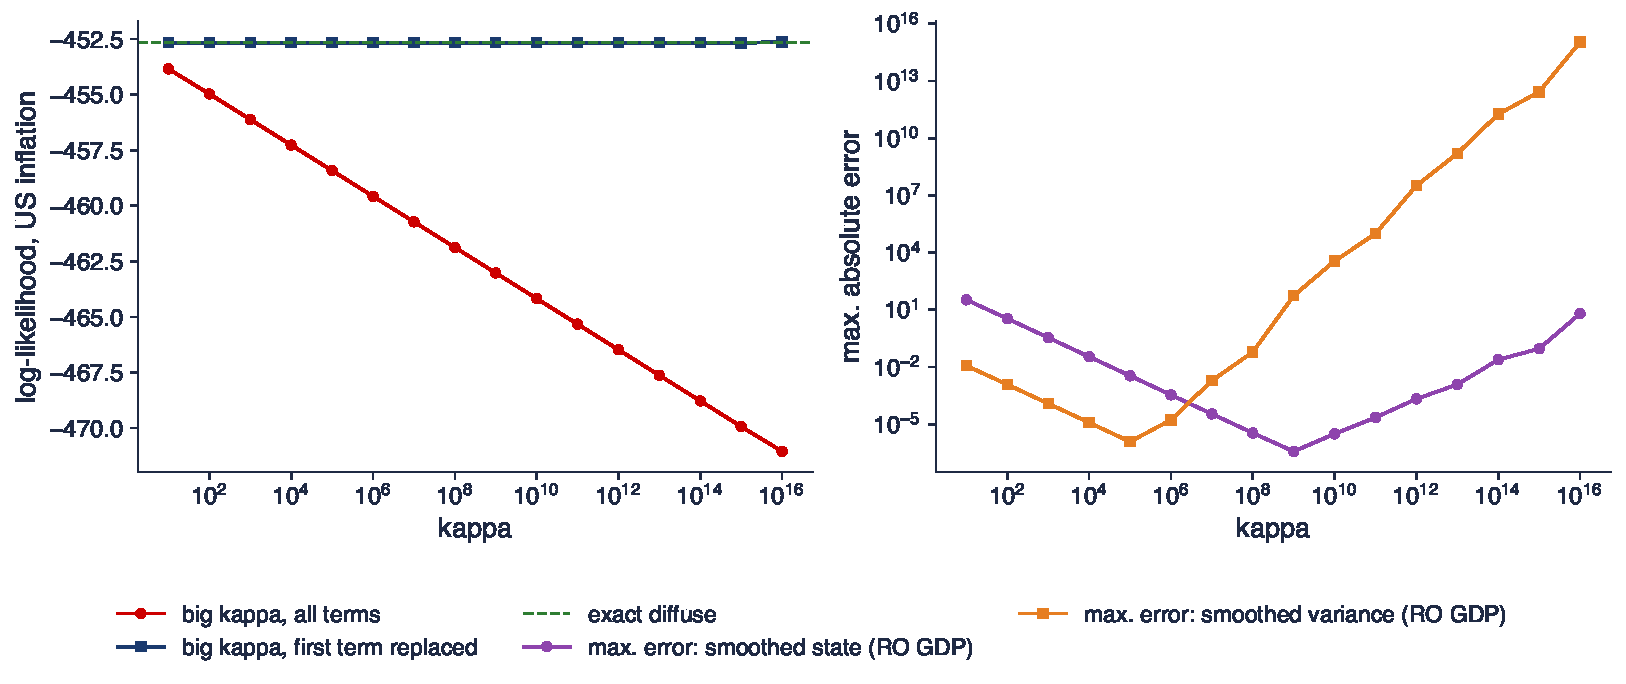
\includegraphics[width=0.97\textwidth,height=0.65\textheight,keepaspectratio]{ats_ch6_diffuse.pdf}
\end{center}
\vspace{-0.25cm}
\begin{itemize}
    \item Stînga: modelul local level pentru inflația deflatorului PIB din SUA, la varianțele ML; dreapta: local linear trend pentru 100$\times$log PIB real al României, $T = 106$; ambele comparate cu filtrul difuz exact
\end{itemize}
\quantlet{ATS\_ch6\_kalman\_mle}{\qlurl{ATS_ch6_kalman_mle}}
\end{frame}

\begin{frame}{Interpretarea inițializării difuze}
\itemsize{\small}
\begin{itemize}
    \item Cu toți termenii, log-verosimilitatea big kappa scade cu $\frac12\ln 10$ la fiecare ordin de mărime al lui $\kappa$: \ensuremath{-}460{,}72 la $\kappa = 10^7$, \ensuremath{-}468{,}78 la $10^{14}$; valoarea exactă este \ensuremath{-}452{,}66
    \item Înlocuirea primului termen cu limita lui difuză repară nivelul (\ensuremath{-}452{,}66 la $10^7$), dar doar pentru că știm că $d = 1$; estimarea ML după $\psi$ nu este afectată, compararea modelelor cu $d$ diferit este
    \item Varianțele netezite: eroarea este 0{,}000012 la $\kappa = 10^4$, 0{,}06 la $10^8$ și $10^{15}$ la $10^{16}$: niciun $\kappa$ nu este sigur simultan pentru stări și pentru varianțe
    \item Regula practică: folosiți filtrul difuz exact ori de cîte ori modelul are stări nestaționare sau fixe necunoscute
\end{itemize}
\end{frame}

\begin{frame}{Recapitulare: modelul liniar gaussian general}
\itemsize{\small}
\begin{itemize}
    \item O singură lemă (condiționarea gaussiană) dă filtrul, netezitorul și netezitorul perturbațiilor
    \item Datele lipsă, frecvențele mixte și observațiile multivariate se tratează în aceleași recursii
    \item Stările nestaționare cer filtrul difuz exact; big kappa denaturează nivelul verosimilității și varianțele netezite
\end{itemize}
\end{frame}


%=============================================================================
\section{Verosimilitatea exactă și maximizarea ei}
%=============================================================================

\begin{frame}{Descompunerea erorilor de predicție, cazul difuz}
\itemsize{\small}
\begin{itemize}
    \item $p(y_1, \dots, y_n) = \prod_t p(y_t | Y_{t-1})$, iar $y_t | Y_{t-1} \sim N(Z_ta_t, F_t)$: verosimilitatea este un produs secundar al filtrului
    \item Log-verosimilitatea difuză \refDK, ec.~(7.4): $\ln L_d = -\frac{np}{2}\ln 2\pi - \frac12\sum_{t=1}^d w_t - \frac12\sum_{t=d+1}^n(\ln|F_t| + v_t'F_t^{-1}v_t)$
    \item $w_t = \ln F_{\infty,t}$ dacă $F_{\infty,t} > 0$, altfel $w_t = \ln F_{*,t} + v_t^2/F_{*,t}$: primele $d$ observații doar fixează stările difuze
    \begin{itemize}
        \item echivalentă cu verosimilitatea marginală din \refdJa\ și cu tratarea stărilor difuze ca parametri ficși, eliminați prin concentrare
    \end{itemize}
    \item Scala: scriem $H_t = \sigma^2H^*_t$, $Q_t = \sigma^2Q^*_t$; atunci $F_t = \sigma^2F^*_t$ și $\hat\sigma^2 = \frac{1}{p(n - d)}\sum_{t>d}v_t'F_t^{*-1}v_t$: un parametru mai puțin în căutarea numerică
\end{itemize}
\end{frame}

\begin{frame}{Maximizarea verosimilității}
\itemsize{\small}
\begin{itemize}
    \item Parametrizăm varianțele prin $\exp(\cdot)$, corelațiile prin $\tanh(\cdot)$, coeficienții AR prin autocorelațiile parțiale: căutare fără restricții, doar modele staționare
    \begin{itemize}
        \item mai multe puncte de pornire: verosimilitățile UC sînt adesea multimodale (MNZ, mai jos)
    \end{itemize}
    \item Scorul într-o singură trecere filtru--netezitor: $\partial\ln L/\partial\psi = \frac12\sum_t\mathrm{tr}\{(\hat\varepsilon_t\hat\varepsilon_t' + \Var(\varepsilon_t|Y_n) - H_t)H_t^{-1}\tfrac{\partial H_t}{\partial\psi}H_t^{-1}\} + \dots$ \refDK, secțiunea 7.3
    \item Algoritmul EM \refSS: pasul E este netezitorul, pasul M are formule explicite pentru $H$ și $Q$; lent lîngă optim, dar robust la puncte de pornire slabe (DFM mari)
    \item Erorile standard: inversa hessianei în $\hat\psi$ (numerică); valabile doar pentru puncte interioare; le raportăm pe scala transformată
    \item Identificarea: unele modele UC sînt echivalente observațional cu modele ARIMA cu mai puțini parametri; verificați forma redusă înainte de a interpreta componentele
\end{itemize}
\end{frame}

\begin{frame}{Local level pentru inflația din SUA: numpy față de statsmodels}
\itemsize{\footnotesize}
\begin{center}
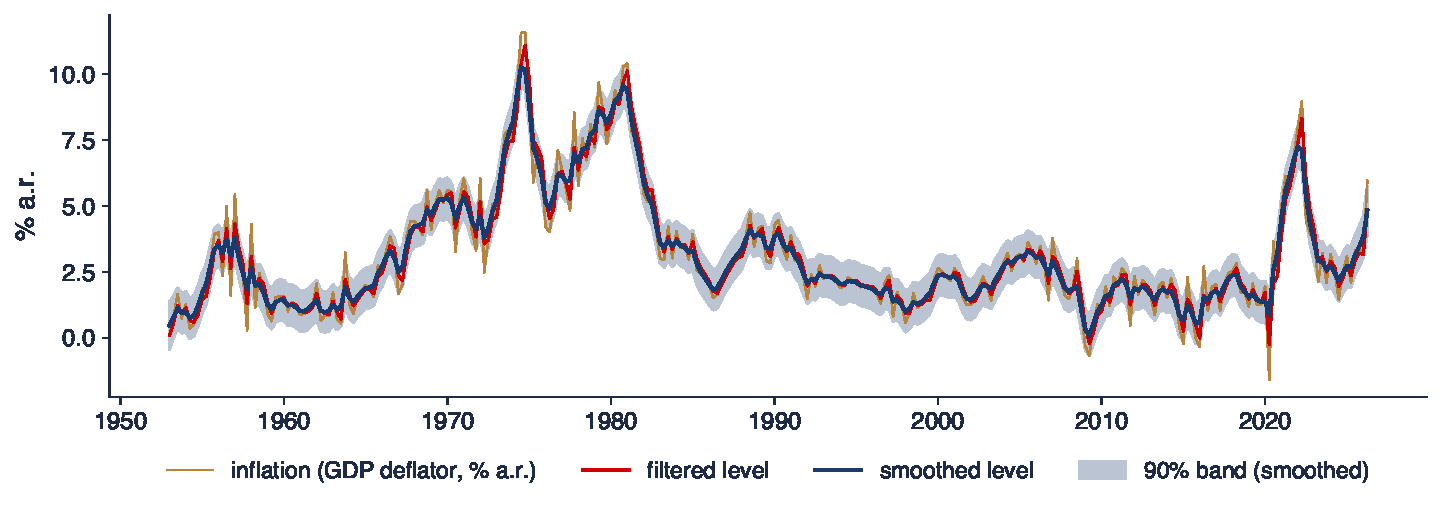
\includegraphics[width=0.97\textwidth,height=0.65\textheight,keepaspectratio]{ats_ch6_local_level.pdf}
\end{center}
\vspace{-0.25cm}
\begin{itemize}
    \item Inflația deflatorului PIB, T1 1953--T2 2026, $T = 294$; ML difuz exact; nivelul netezit cu o bandă de 90\% și nivelul unilateral (filtrat)
\end{itemize}
\quantlet{ATS\_ch6\_kalman\_mle}{\qlurl{ATS_ch6_kalman_mle}}
\end{frame}

\begin{frame}{Interpretarea estimațiilor local level}
\itemsize{\small}
\begin{itemize}
    \item numpy: $\hat\sigma^2_\varepsilon = 0{,}517$, $\hat\sigma^2_\eta = 0{,}453$, $\hat q = 0{,}877$; statsmodels: 0{,}517 și 0{,}453: același optim
    \item Log-verosimilitățile \ensuremath{-}452{,}66 și \ensuremath{-}451{,}74: diferă exact cu $\frac12\ln 2\pi = 0{,}919$, constanta pe care \texttt{statsmodels} o omite pentru observația difuză ($d = 1$)
    \item Cîștigul în starea staționară este 0{,}596: fiecare trimestru nou mută estimația nivelului cu 60\% din surpriză; inflația este mai aproape de un mers aleator decît de un zgomot alb în jurul unei medii
    \item Ultimul nivel netezit este 4{,}83\% (abatere standard 0{,}55): la finalul eșantionului estimațiile netezite și filtrate coincid, la fel și incertitudinea lor
    \item O singură varianță constantă pentru 1953--2026 este neplauzibilă (Marea Inflație, Marea Moderație): de aici modelul UC-SV din ultima secțiune
\end{itemize}
\end{frame}

\begin{frame}{Inferența la frontieră: problema pile-up}
\itemsize{\small}
\begin{itemize}
    \item Modelul local level cu $q = \sigma^2_\eta/\sigma^2_\varepsilon$: estimația ML este exact zero cu probabilitate pozitivă chiar dacă $q > 0$ \refSH
    \begin{itemize}
        \item scorul în $q = 0$ este adesea negativ, pentru că un trend neted se potrivește datelor mai bine decît unul care rătăcește puțin
    \end{itemize}
    \item Consecințele
    \begin{itemize}
        \item intervalul de încredere calculat din hessiană nu este valid
        \item testul LR pentru $q = 0$ nu este $\chi^2_1$, nici măcar $\frac12\chi^2_0 + \frac12\chi^2_1$: modelul sub alternativă este nestaționar
        \item remedii: estimarea median-nedeplasată a varianței coeficienților \refSWa; bootstrap parametric pentru statistica LR (secțiunea TVP); distribuții a priori care țin $q$ departe de zero
    \end{itemize}
    \item Aceeași problemă apare în regresiile TVP (este coeficientul constant?) și în modelele UC (este trendul determinist?)
\end{itemize}
\end{frame}

\begin{frame}{Cît de des este varianța estimată a nivelului exact zero?}
\itemsize{\footnotesize}
\begin{center}
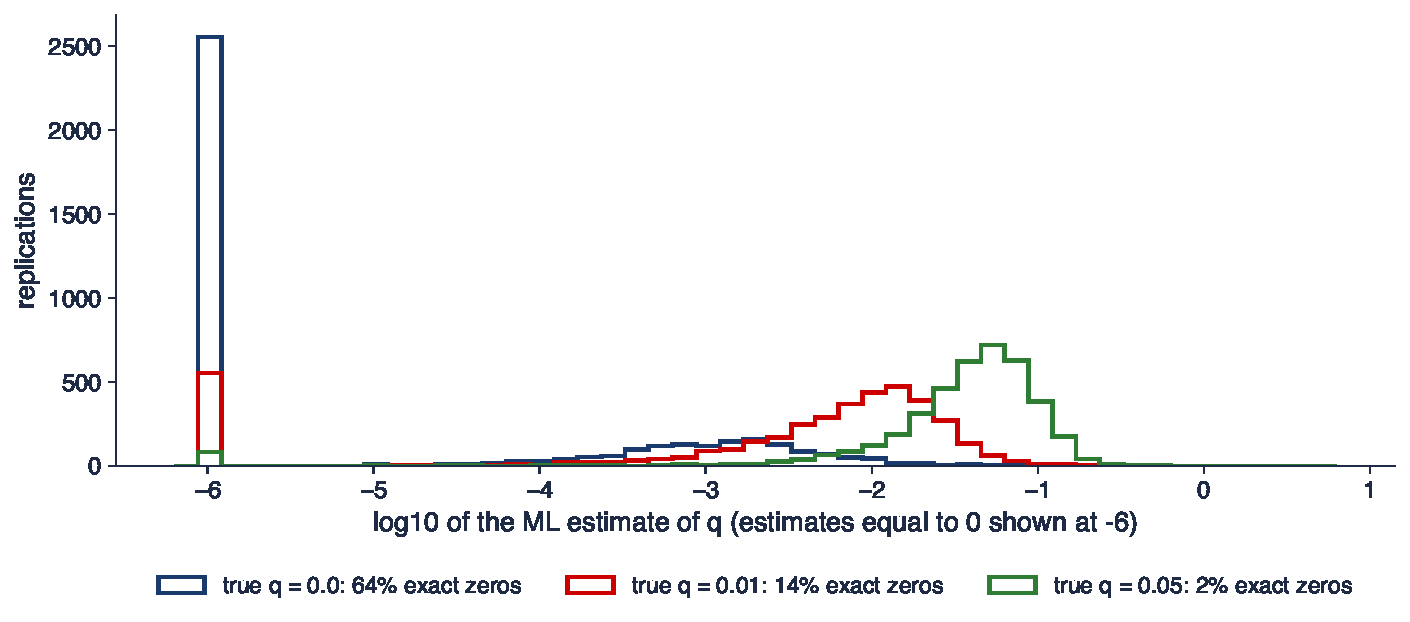
\includegraphics[width=0.97\textwidth,height=0.65\textheight,keepaspectratio]{ats_ch6_pileup.pdf}
\end{center}
\vspace{-0.25cm}
\begin{itemize}
    \item Cîte 4\,000 de serii local level simulate de lungime $T = 100$ pentru fiecare $q$ adevărat; ML pentru $q$ pe o grilă fină, cu $\sigma^2_\varepsilon$ eliminat prin concentrare
\end{itemize}
\quantlet{ATS\_ch6\_kalman\_mle}{\qlurl{ATS_ch6_kalman_mle}}
\end{frame}

\begin{frame}{Interpretarea simulării pile-up}
\itemsize{\small}
\begin{itemize}
    \item Pentru $q = 0$ adevărat: 64\% dintre estimații sînt exact zero; restul se împrăștie pe mai multe ordine de mărime
    \item Pentru $q = 0{,}01$: tot 14\% zerouri; mediana estimațiilor este 0{,}0077; pentru $q = 0{,}05$: 2\% zerouri
    \item Un $\hat\sigma^2_\eta = 0$ raportat nu este deci o dovadă a unui nivel constant; o valoare pozitivă mică este compatibilă cu un nivel determinist
    \item Raportați verosimilitatea profil sau distribuția a posteriori a lui $q$, nu o estimație punctuală cu o eroare standard din hessiană
\end{itemize}
\end{frame}

\begin{frame}{Recapitulare: verosimilitatea exactă}
\itemsize{\small}
\begin{itemize}
    \item Filtrul dă verosimilitatea gaussiană; cu stări difuze, primii $d$ termeni sînt înlocuiți cu limitele lor difuze
    \item Concentrați scala, parametrizați fără restricții, folosiți mai multe puncte de pornire și verificați cifrele cu o a doua implementare
    \item Varianțele apropiate de zero se acumulează în zero: erorile standard și testele $\chi^2$ nu funcționează la frontieră
\end{itemize}
\end{frame}


%=============================================================================
\section{Spațiul stărilor bayesian: simulation smoothing și eșantionare Gibbs}
%=============================================================================

\begin{frame}{Eșantionarea stărilor}
\itemsize{\footnotesize}
\begin{columns}[T]
\begin{column}{0.3\textwidth}
\centering
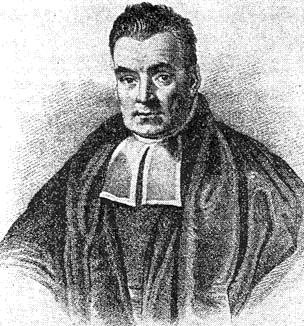
\includegraphics[height=0.34\textheight]{ch6_bayes.png}\\[1mm]
\imgcap{Portret identificat tradițional cu Thomas Bayes (identificare incertă)}
\imgcredit{https://commons.wikimedia.org/wiki/File:Thomas_Bayes.gif}{Portret: autor necunoscut; domeniu public; Wikimedia Commons}
\end{column}
\begin{column}{0.68\textwidth}
\begin{itemize}
    \item Ținta: $p(\alpha_1, \dots, \alpha_n, \psi | Y_n)$; filtrul dă $p(\alpha_t | Y_t, \psi)$ doar pentru un $t$ și un $\psi$
    \item Eșantionatorul Gibbs: alternăm $\alpha_{1:n} \sim p(\alpha_{1:n} | \psi, Y_n)$ și $\psi \sim p(\psi | \alpha_{1:n}, Y_n)$; dată fiind starea, $\psi$ este adesea o problemă de regresie conjugată
    \item Incertitudinea despre $\psi$ intră în benzile stărilor (benzile ML o ignoră)
    \item Funcțiile de traiectorii întregi devin ușor de calculat: data unui maxim, probabilitatea ca un trend să rămînă într-o bandă-țintă
    \item Eșantionarea întregii traiectorii într-un singur bloc (nu cîte un $\alpha_t$) asigură o bună amestecare (mixing) a eșantionatorului
\end{itemize}
\end{column}
\end{columns}
\end{frame}

\begin{frame}{Filtrare înainte, eșantionare înapoi}
\itemsize{\small}
\begin{itemize}
    \item Factorizarea: $p(\alpha_{1:n} | Y_n) = p(\alpha_n | Y_n)\prod_{t=1}^{n-1}p(\alpha_t | \alpha_{t+1}, Y_t)$ (proprietatea Markov a stării)
    \item Înainte: rulăm filtrul și păstrăm $a_{t|t}, P_{t|t}$; extragem $\alpha_n \sim N(a_{n|n}, P_{n|n})$ \refCK, \refFS
    \item Înapoi: $\alpha_t | \alpha_{t+1}, Y_t \sim N(m_t, S_t)$ din lemă, cu cîștigul de netezire $G_t = P_{t|t}T_t'P_{t+1}^{-1}$ ($m_t$, $S_t$: media și varianța condiționate):
    \begin{itemize}
        \item $m_t = a_{t|t} + G_t(\alpha_{t+1} - c_t - T_ta_{t|t})$, $\quad S_t = P_{t|t} - G_tT_tP_{t|t}$
    \end{itemize}
    \item Probleme: $P_{t+1}$ este singulară cînd $R_tQ_tR_t'$ este singulară (laguri în stare): folosim doar rîndurile cu șocuri; $n$ extrageri de dimensiune $m$
    \item Același rezultat ca pasul Gibbs din eșantionatoarele BVAR și DFM din \atschlink{https://danpele.github.io/Advanced-Time-Series/RO/Cursuri/capitol5_bvar_modele_factoriale_nowcasting.pdf}{Capitolul 5}
\end{itemize}
\end{frame}

\begin{frame}{Simulation smoother-ul Durbin--Koopman}
\itemsize{\small}
\begin{itemize}
    \item Ideea \refDKa: $\alpha - \hat\alpha(y)$ are aceeași distribuție condiționată pentru orice $y$ (modelul gaussian): o simulăm o singură dată din model
    \item Algoritmul (corecția mediei):
    \begin{itemize}
        \item 1. extragem $\alpha^+_{1:n}, y^+_{1:n}$ din model (șocuri și stare inițială); păstrăm structura valorilor lipsă din $y$
        \item 2. rulăm o singură dată netezitorul stărilor pe $y - y^+$ (termeni liberi nuli): $\hat\alpha(y - y^+) = \hat\alpha(y) - \hat\alpha(y^+)$
        \item 3. $\tilde\alpha = \alpha^+ + \hat\alpha(y) - \hat\alpha(y^+)$ este o extragere din $p(\alpha | Y_n)$
    \end{itemize}
    \item Este nevoie doar de netezitorul mediei: fără inversarea lui $P_{t|t}$, fără probleme de singularitate, stările difuze sînt tratate de netezitorul difuz exact (demonstrația: \atsapplink{atsapp2}{atssrc2}{Anexa})  % applink: exactitatea simulation smoother
    \item Precursor: simulation smoother-ul perturbațiilor din \refdJS; aceeași idee pentru perturbațiile $\varepsilon_t, \eta_t$
\end{itemize}
\end{frame}

\begin{frame}{Eșantionarea pe baza matricei de precizie}
\itemsize{\small}
\begin{itemize}
    \item Scriem modelul matriceal \refCJ: $y = X\alpha + \varepsilon$, $D\alpha = \eta$
    \begin{itemize}
        \item $D$: o matrice de diferențe în bandă (diferențe de ordinul întîi pentru un mers aleator)
        \item atunci $\alpha | y \sim N(\hat\alpha, K^{-1})$, cu $K = D'\Sigma_\eta^{-1}D + X'\Sigma_\varepsilon^{-1}X$
    \end{itemize}
    \item $K$ este în bandă (tridiagonală pentru un mers aleator): un singur factor Cholesky în bandă $K = U'U$ costă $O(n)$
    \begin{itemize}
        \item $\alpha$, $y$: toate stările și observațiile așezate una sub alta; $X$: matricea bloc-diagonală a lui $Z_t$; $\Sigma_\varepsilon$, $\Sigma_\eta$: covarianțele zgomotelor; $K$: precizia a posteriori (inversa covarianței)
        \item $\hat\alpha$ rezolvă $K\hat\alpha = X'\Sigma_\varepsilon^{-1}y$; o extragere este $\hat\alpha + U^{-1}z$, $z \sim N(0, I)$
    \end{itemize}
    \item Varianțele variabile în timp (volatilitatea stochastică) schimbă doar ponderile de pe diagonală: ideal în eșantionatoarele Gibbs pentru UC-SV și SV
    \item Trei eșantionatoare, o singură țintă: FFBS, DK și eșantionarea pe baza preciziei extrag din aceeași $p(\alpha | Y_n, \psi)$; diferă prin cost și generalitate
\end{itemize}
\end{frame}

\begin{frame}{Trei eșantionatoare pentru aceeași distribuție a posteriori}
\itemsize{\footnotesize}
\begin{center}
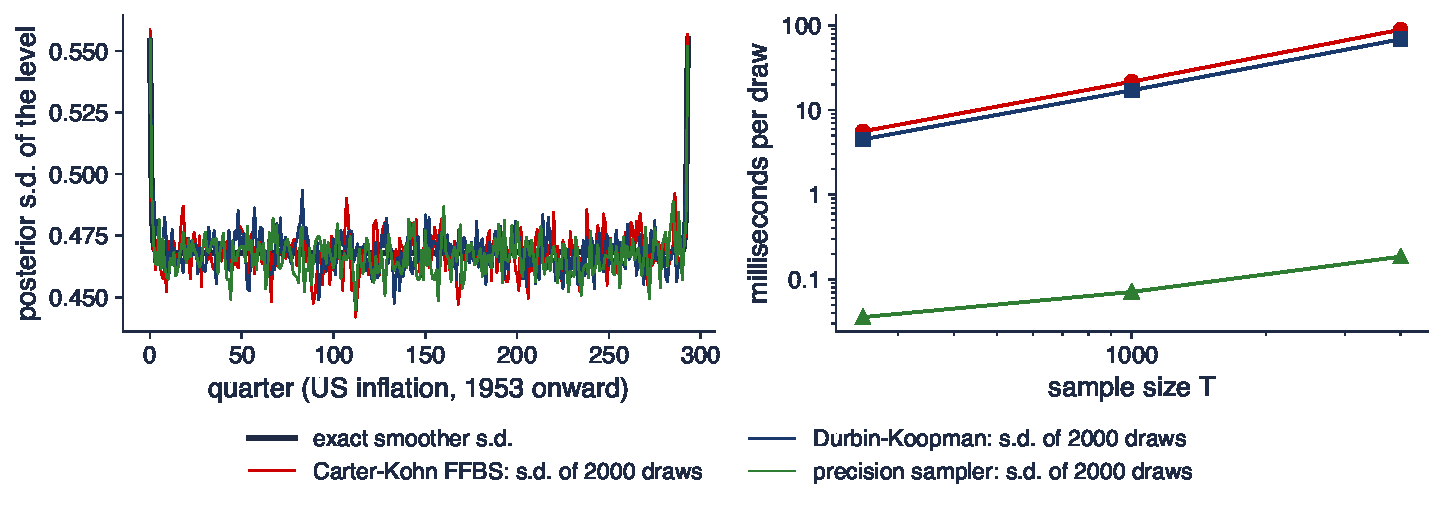
\includegraphics[width=0.97\textwidth,height=0.65\textheight,keepaspectratio]{ats_ch6_simsmoother.pdf}
\end{center}
\vspace{-0.25cm}
\begin{itemize}
    \item Local level pentru inflația din SUA la varianțele ML, a priori propriu $\mu_1 \sim N(y_1, 100)$; stînga: abaterea standard a 2\,000 de extrageri față de netezitorul exact; dreapta: timpul pe extragere pentru eșantioane simulate
\end{itemize}
\quantlet{ATS\_ch6\_simulation\_smoother}{\qlurl{ATS_ch6_simulation_smoother}}
\end{frame}

\begin{frame}{Interpretarea celor trei eșantionatoare}
\itemsize{\small}
\begin{itemize}
    \item Rapoartele dintre abaterea standard a extragerilor și cea exactă se află în [0{,}94; 1{,}05] (FFBS), [0{,}96; 1{,}05] (DK) și [0{,}95; 1{,}04] (precizie): doar zgomot Monte Carlo
    \item Cea mai mare eroare a mediilor extragerilor: 0{,}031; 0{,}027; 0{,}039, de ordinul erorii standard Monte Carlo
    \item Pentru $T = 4000$: 89{,}2 ms (FFBS), 68{,}8 ms (DK), 0{,}19 ms (precizie) pe extragere; toate sînt liniare în $T$, rezolvarea în bandă nu are buclă Python
    \item Alegeți DK pentru modele generale cu stări difuze și eșantionarea pe baza preciziei pentru mersuri aleatoare cu varianțe variabile în timp
\end{itemize}
\end{frame}

\begin{frame}{Un eșantionator Gibbs pentru modelul local level}
\itemsize{\small}
\begin{itemize}
    \item Modelul: $y_t = \mu_t + \varepsilon_t$, $\mu_{t+1} = \mu_t + \eta_t$; $\mu_t$: nivelul; $IG(a_0, b_0)$: distribuția a priori inverse gamma cu formă $a_0$ și scală $b_0$; $q = \sigma^2_\eta/\sigma^2_\varepsilon$
    \item Blocul 1: $\mu_{1:n} | \sigma^2_\varepsilon, \sigma^2_\eta, Y_n$ prin simulation smoother-ul DK (cu $\mu_1$ difuz exact)
    \item Blocul 2: $\sigma^2_\varepsilon | \mu, Y_n \sim IG(a_0 + \frac n2, b_0 + \frac12\sum_t(y_t - \mu_t)^2)$; $\sigma^2_\eta | \mu \sim IG(a_0 + \frac{n-1}{2}, b_0 + \frac12\sum_t(\Delta\mu_t)^2)$
    \item A priori $IG(2{,}5; 0{,}25)$ pentru ambele: propriu, slab și exclude exact $\sigma^2_\eta = 0$
    \begin{itemize}
        \item distribuția a priori nu este neutră lîngă frontieră: un IG conjugat împinge în sus varianțele mici; parametrizarea necentrată din \refFSW\ permite în schimb o distribuție a priori Normală pentru $\pm\sigma_\eta$
    \end{itemize}
    \item Convergența: grafice ale traiectoriilor, mai multe lanțuri, factorul de ineficiență $1 + 2\sum_k\rho_k$ (ponderi Parzen): numărul de extrageri care valorează cît o extragere independentă \refKSC
\end{itemize}
\end{frame}

\begin{frame}{Distribuția a posteriori Gibbs a raportului semnal--zgomot}
\itemsize{\footnotesize}
\begin{center}
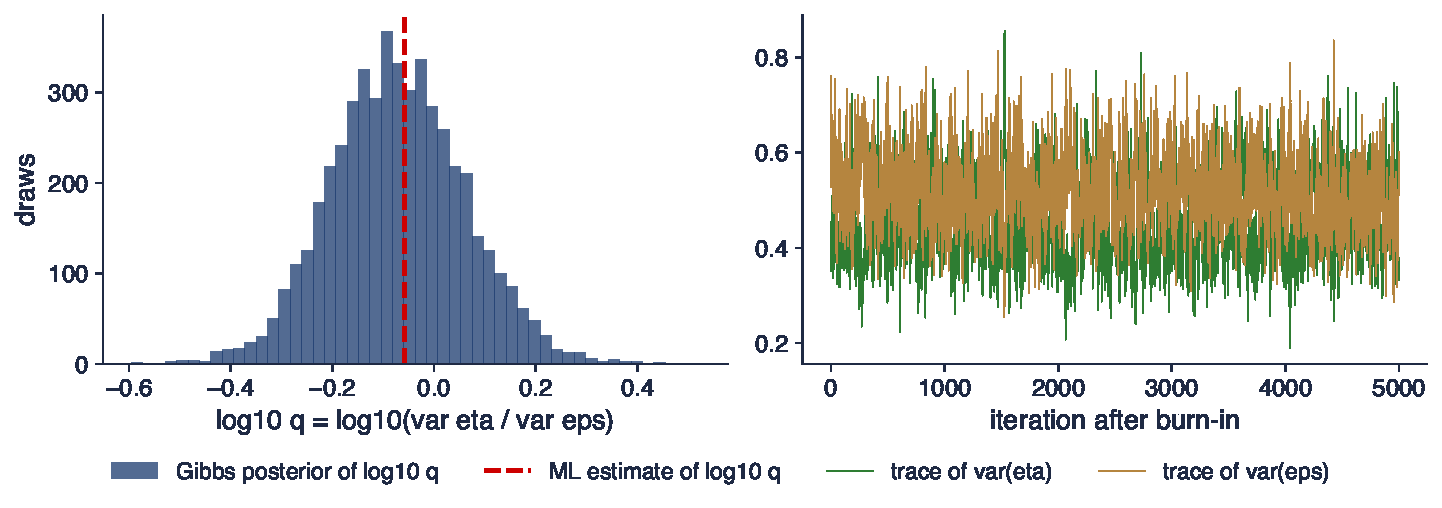
\includegraphics[width=0.97\textwidth,height=0.65\textheight,keepaspectratio]{ats_ch6_gibbs_ll.pdf}
\end{center}
\vspace{-0.25cm}
\begin{itemize}
    \item Inflația din SUA, local level, 5\,000 de extrageri după perioada de ardere; stînga: distribuția a posteriori a lui $\log_{10}q$ și valoarea ML; dreapta: traiectoriile celor două varianțe
\end{itemize}
\quantlet{ATS\_ch6\_simulation\_smoother}{\qlurl{ATS_ch6_simulation_smoother}}
\end{frame}

\begin{frame}{Interpretarea rezultatelor Gibbs}
\itemsize{\small}
\begin{itemize}
    \item Mediana a posteriori a lui $q$: 0{,}84, intervalul de credibilitate de 90\% [0{,}52; 1{,}42]; ML: 0{,}88
    \item Mediile a posteriori 0{,}515 și 0{,}441 față de ML 0{,}517 și 0{,}453: cu $n = 294$, a priori contează foarte puțin departe de frontieră
    \item Factorii de ineficiență 9{,}9 și 11{,}3: extragerile varianțelor moștenesc autocorelația extragerilor stărilor
    \item Intervalul pentru $q$ exclude zero: trendul inflației din SUA se mișcă, dar capătul superior al intervalului este de 2{,}7 ori mai mare decît cel inferior
\end{itemize}
\end{frame}

\begin{frame}{Recapitulare: spațiul stărilor bayesian}
\itemsize{\small}
\begin{itemize}
    \item Gibbs: stările ca un singur bloc, dați parametrii; parametrii, date stările
    \item FFBS, simulation smoother-ul DK și eșantionarea pe baza preciziei extrag din aceeași distribuție
    \item Distribuțiile a priori regularizează problemele de frontieră, dar trebuie raportate și variate
\end{itemize}
\end{frame}


%=============================================================================
\section{Volatilitatea stochastică}
%=============================================================================

\begin{frame}{Modelul de volatilitate stochastică}
\itemsize{\footnotesize}
\begin{columns}[T]
\begin{column}{0.3\textwidth}
\centering
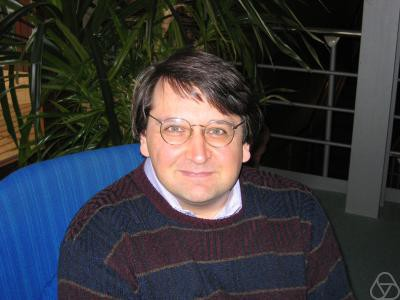
\includegraphics[height=0.30\textheight]{ch6_shephard_2004.jpg}\\[1mm]
\imgcap{Neil Shephard, 2004}
\imgcredit{https://commons.wikimedia.org/wiki/File:Shephard,_Neil_(1964).jpeg}{Foto: Renate Schmid (2004), MFO; CC BY-SA 2.0 de; Wikimedia Commons}
\end{column}
\begin{column}{0.68\textwidth}
\begin{itemize}
    \item $y_t = \exp(h_t/2)\,\epsilon_t$, $\quad h_{t+1} = \mu + \phi(h_t - \mu) + \sigma_\eta\eta_t$, $\quad \epsilon_t, \eta_t \sim$ i.i.d. $N(0, 1)$ \refTay
    \item $h_t$: logaritmul varianței, o stare latentă AR(1); $\phi$: persistența; $\sigma_\eta$: volatilitatea volatilității; $\exp(\mu/2)$: volatilitatea tipică
    \item Un model în spațiul stărilor cu ecuația de măsurare neliniară: filtrul Kalman nu se aplică direct
    \item Corespondentul în timp continuu: logaritmul varianței ca proces Ornstein--Uhlenbeck (evaluarea opțiunilor, măsurile realizate din \atschlink{https://danpele.github.io/Advanced-Time-Series/RO/Cursuri/capitol8_volatilitate_avansata.pdf}{Capitolul 8})
\end{itemize}
\end{column}
\end{columns}
\end{frame}

\begin{frame}{Volatilitatea stochastică nu este GARCH (1/2)}
\itemsize{\small}
\begin{itemize}
    \item GARCH \refBol: $\sigma^2_t = \omega + \alpha y^2_{t-1} + \beta\sigma^2_{t-1}$, $\omega > 0$, $\alpha, \beta \ge 0$
    \begin{itemize}
        \item $\sigma^2_t$ este cunoscută la $t-1$ (o funcție de randamentele trecute): o singură sursă de aleatoriu
        \item verosimilitatea este un produs de densități cunoscute: o singură trecere, ML exact
    \end{itemize}
    \item SV: $h_t$ are propriul șoc $\eta_t$; chiar cu toate randamentele trecute, varianța de azi este incertă
    \begin{itemize}
        \item $p(y_{1:n} | \psi) = \int\prod_t N(y_t; 0, e^{h_t})\,p(h_{1:n} | \psi)\,dh_{1:n}$: o integrală $n$-dimensională fără formă închisă
    \end{itemize}
    \item Compararea pe scala verosimilității este posibilă doar după calculul integralei: filtrul de particule (secțiunea următoare) sau eșantionarea prin importanță \refKSC
\end{itemize}
\end{frame}

\begin{frame}{Volatilitatea stochastică nu este GARCH (2/2)}
\itemsize{\small}
\begin{itemize}
    \item Momentele, cu $\sigma^2_h = \sigma^2_\eta/(1 - \phi^2)$ varianța necondiționată a lui $h_t$
    \begin{itemize}
        \item kurtosis-ul lui $y_t$: $3\exp(\sigma^2_h) > 3$ chiar cu $\epsilon_t$ gaussian: cozile groase provin din varianța aleatoare
        \item $\Corr(y^2_t, y^2_{t-k}) = (e^{\sigma^2_h\phi^k} - 1)/(3e^{\sigma^2_h} - 1)$: volatility clustering care scade odată cu $\phi^k$
    \end{itemize}
    \item Efectul de levier intră prin $\Corr(\epsilon_t, \eta_t) = \rho < 0$ \refOCSN; GARCH are nevoie de un termen asimetric pentru același efect
\end{itemize}
\end{frame}

\begin{frame}{O formă liniară în spațiul stărilor: logaritmul pătratelor randamentelor}
\itemsize{\small}
\begin{itemize}
    \item $y^*_t = \ln y^2_t = h_t + \xi_t$, $\xi_t = \ln\epsilon^2_t$: liniar în $h_t$, dar $\xi_t$ are o lege $\ln\chi^2_1$ cu media $-1{,}2704$ și varianța $\pi^2/2 \approx 4{,}93$
    \item QML \refHRS: rulăm filtrul Kalman ca și cum $\xi_t$ ar fi $N(-1{,}2704; \pi^2/2)$; consistent, dar ineficient
    \begin{itemize}
        \item $y^*_t$ este ARMA(1,1): $\Corr(y^*_t, y^*_{t-k}) = \phi^k\sigma^2_h/(\sigma^2_h + \pi^2/2)$, mică pentru că zgomotul domină semnalul
    \end{itemize}
    \item Randamentele nule: $\ln 0 = -\infty$; folosim $y^*_t = \ln(y^2_t + c)$ cu o constantă mică $c$ (aici $c = 10^{-3}\Var(y)$, scalată la serie)
    \item Extensia multivariată a aceleiași idei: modele SV factoriale \refHRS
\end{itemize}
\end{frame}

\begin{frame}{Mixtura KSC: un model condiționat gaussian}
\itemsize{\footnotesize}
\begin{columns}[T]
\begin{column}{0.55\textwidth}
\begin{itemize}
    \item \refKSC: aproximăm $\ln\chi^2_1$ printr-o mixtură de șapte distribuții Normale; dată componenta $s_t$, modelul este liniar și gaussian
    \item $y^*_t = h_t + m_{s_t} - 1{,}2704 + \sqrt{v_{s_t}}\,u_t$, $u_t \sim N(0, 1)$, $P(s_t = i) = p_i$; $s_t \in \{1, \dots, 7\}$: componenta; $p_i$, $m_i$, $v_i$: probabilitatea, media și varianța ei (tabelul)
    \item Media mixturii \ensuremath{-}1{,}2704 și varianța 4{,}935, față de $-1{,}2704$ și 4,935 pentru legea exactă
    \item Eroarea de aproximare rămasă se poate elimina prin reponderarea extragerilor (ponderi de importanță) \refKSC; mixturi mai fine cu 10 componente \refOCSN
\end{itemize}
\end{column}
\begin{column}{0.42\textwidth}
\begin{center}
\scriptsize
\begin{tabular}{cccc}
\toprule
$i$ & $p_i$ & $m_i$ & $v_i$ \\
\midrule
1 & $0{,}00730$ & $-10{,}12999$ & $5{,}79596$ \\
2 & $0{,}10556$ & $-3{,}97281$ & $2{,}61369$ \\
3 & $0{,}00002$ & $-8{,}56686$ & $5{,}17950$ \\
4 & $0{,}04395$ & $2{,}77786$ & $0{,}16735$ \\
5 & $0{,}34001$ & $0{,}61942$ & $0{,}64009$ \\
6 & $0{,}24566$ & $1{,}79518$ & $0{,}34023$ \\
7 & $0{,}25750$ & $-1{,}08819$ & $1{,}26261$ \\
\bottomrule
\end{tabular}
\end{center}
\begin{itemize}
    \item Sursa: \refKSC, tabelul 4
\end{itemize}
\end{column}
\end{columns}
\end{frame}

\begin{frame}{Legea log chi-pătrat și aproximările ei}
\itemsize{\footnotesize}
\begin{center}
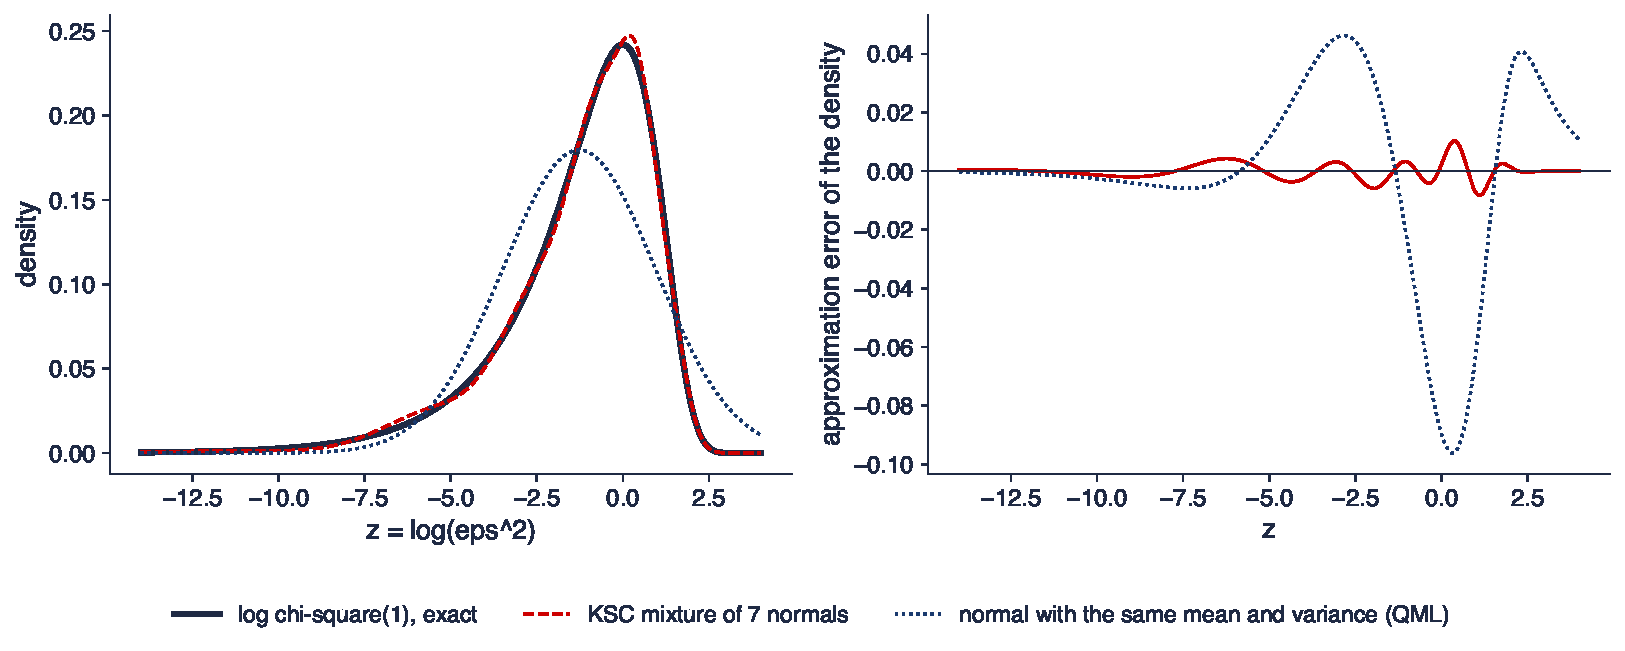
\includegraphics[width=0.97\textwidth,height=0.65\textheight,keepaspectratio]{ats_ch6_ksc.pdf}
\end{center}
\vspace{-0.25cm}
\begin{itemize}
    \item Stînga: densitatea lui $\ln\epsilon^2$ (exactă), mixtura KSC și distribuția Normală cu aceleași două momente folosită de QML; dreapta: cele două erori de aproximare
\end{itemize}
\quantlet{ATS\_ch6\_stochastic\_volatility}{\qlurl{ATS_ch6_stochastic_volatility}}
\end{frame}

\begin{frame}{Interpretarea aproximării prin mixtură}
\itemsize{\small}
\begin{itemize}
    \item Legea are o asimetrie puternică la stînga: randamentele mici produc valori foarte negative pentru $\ln y^2_t$; aproximarea prin distribuția Normală ratează atît asimetria, cît și vîrful
    \item Cea mai mare eroare a densității: 0{,}010 pentru mixtură, 0{,}096 pentru distribuția Normală (QML)
    \item QML tratează un zgomot asimetric ca pe unul simetric: filtrul reacționează excesiv la randamentele apropiate de zero; mixtura corectează acest lucru cu prețul unui bloc Gibbs suplimentar
\end{itemize}
\end{frame}

\begin{frame}{Eșantionarea Gibbs a modelului SV}
\itemsize{\small}
\begin{itemize}
    \item Blocul 1: $s_t | y^*_t, h_t$ independent, $P(s_t = i) \propto p_i\,N(y^*_t - h_t;\ m_i - 1{,}2704, v_i)$
    \item Blocul 2: $h_{1:n} | s, \psi, y^*$ într-o singură extragere: un model liniar gaussian cu varianțe de măsurare cunoscute și variabile în timp $v_{s_t}$ (precizie sau DK)
    \item Blocul 3: $\sigma^2_\eta | h, \mu, \phi$ invers gamma; $\phi$ prin Metropolis--Hastings, cu regresia AR(1) ca propunere; $\mu$ din distribuția Normală
    \item Distribuțiile a priori \refKSC: $(\phi + 1)/2 \sim \mathrm{Beta}(20; 1{,}5)$, $\sigma^2_\eta \sim IG(2{,}5; 0{,}025)$, $\mu \sim N(0, 10)$
    \item Eșantionatoarele cu o singură mișcare (cîte un $h_t$, \refJPR) au o amestecare (mixing) foarte lentă, pentru că valorile consecutive $h_t$ sînt puternic corelate: eșantionați traiectoria ca bloc
\end{itemize}
\end{frame}

\begin{frame}{Volatilitatea stochastică pentru S\&P 500 și BET}
\itemsize{\footnotesize}
\begin{center}
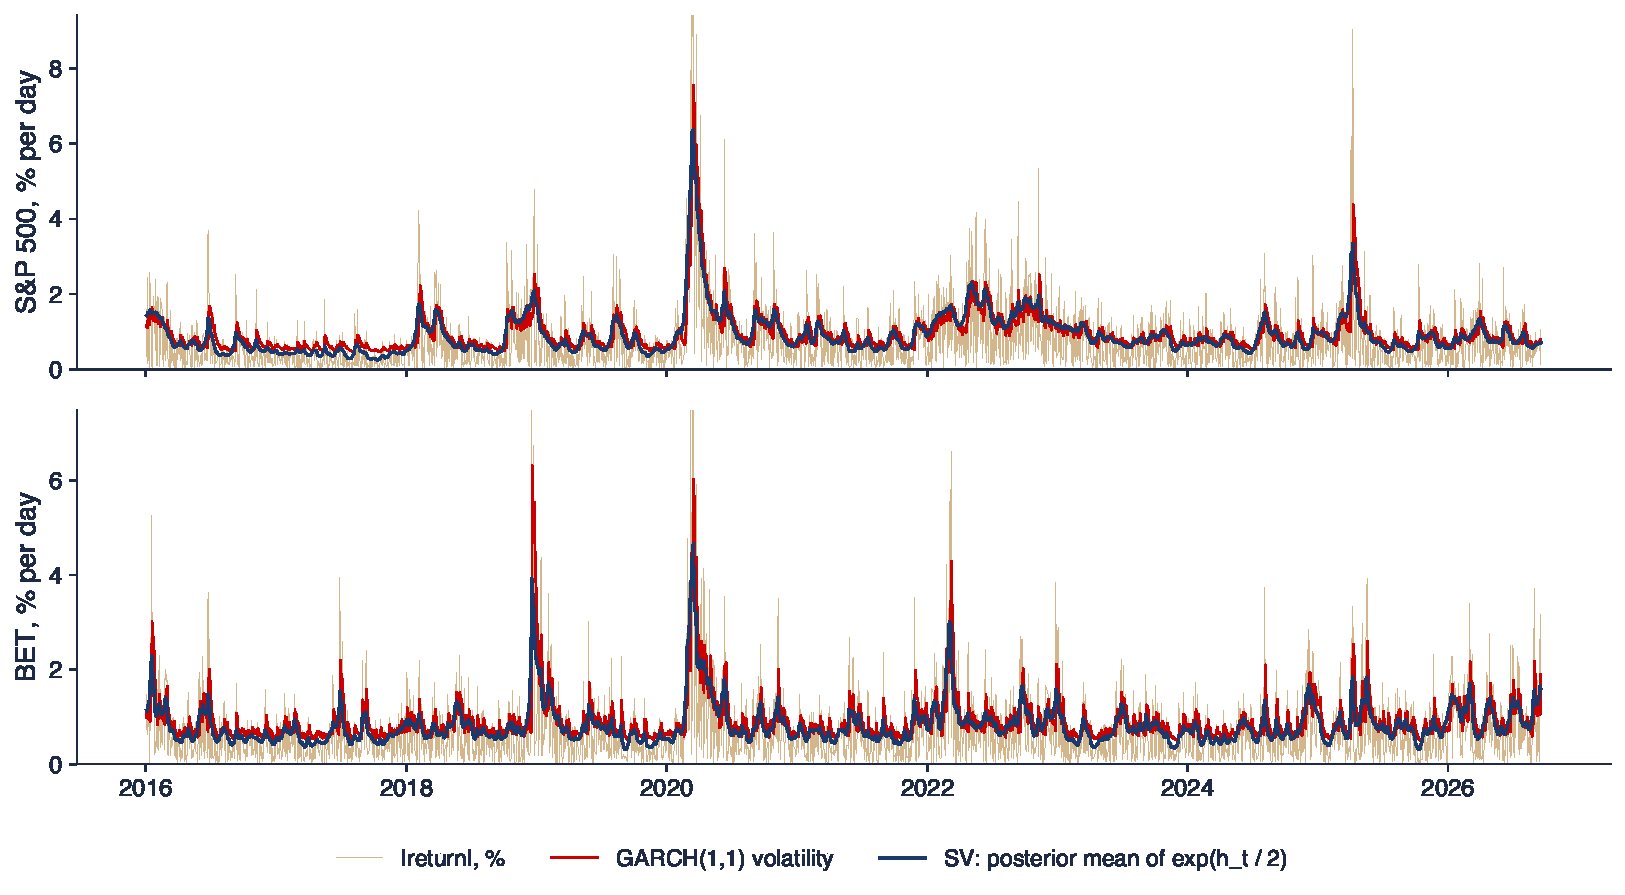
\includegraphics[width=0.97\textwidth,height=0.65\textheight,keepaspectratio]{ats_ch6_sv.pdf}
\end{center}
\vspace{-0.25cm}
\begin{itemize}
    \item Randamente logaritmice zilnice în \%, centrate, 2016--2026 ($T = 2692$ și 2675); eșantionatorul Gibbs KSC, 20\,000 de extrageri; GARCH(1,1) prin ML pe aceleași date
\end{itemize}
\quantlet{ATS\_ch6\_stochastic\_volatility}{\qlurl{ATS_ch6_stochastic_volatility}}
\end{frame}

\begin{frame}{Interpretarea estimațiilor SV}
\itemsize{\footnotesize}
\begin{center}
\footnotesize
\begin{tabular}{lcccccc}
\toprule
Indice & $\phi$ & $\sigma_\eta$ & $\mu$ & inef. $\phi$, $\sigma_\eta$ & GARCH $\alpha + \beta$ & corel. vol. \\
\midrule
S\&P 500 & 0{,}963 & 0{,}289 & \ensuremath{-}0{,}465 & 49 / 98 & 0{,}967 & 0{,}91 \\
BET & 0{,}914 & 0{,}393 & \ensuremath{-}0{,}624 & 58 / 87 & 0{,}952 & 0{,}84 \\
\bottomrule
\end{tabular}
\end{center}
\begin{itemize}
    \item Intervalele de 90\% pentru $\phi$: [0{,}950; 0{,}975] (S\&P 500), [0{,}888; 0{,}938] (BET): logaritmul varianței este foarte persistent, ca în \refKSC
    \item Cele două traiectorii ale volatilității sînt apropiate (corelația din ultima coloană), dar SV reacționează mai puțin decît GARCH la un singur randament mare, la care varianța GARCH sare cu $\alpha y^2_{t-1}$
    \item Factorii de ineficiență mari pentru $\sigma_\eta$ sînt tipici: $\sigma_\eta$ și traiectoria $h_{1:n}$ sînt puternic dependente; sînt necesare lanțuri lungi sau tehnici de interweaving
    \item Kurtosis-ul randamentelor: 19{,}5 (S\&P 500) și 20{,}8 (BET); cu $\epsilon_t$ gaussian, SV explică doar o parte (extensia uzuală: erori SV-$t$)
\end{itemize}
\end{frame}

\begin{frame}{Recapitulare: volatilitatea stochastică}
\itemsize{\small}
\begin{itemize}
    \item SV adaugă un șoc varianței: verosimilitatea este o integrală după traiectoria volatilității
    \item Logaritmul pătratelor randamentelor face modelul liniar; mixtura KSC îl face condiționat gaussian, deci întreaga traiectorie se poate extrage într-un singur bloc
    \item Pe randamentele zilnice ale indicilor, SV și GARCH dau traiectorii apropiate ale volatilității, dar reacții diferite la un singur randament mare
\end{itemize}
\end{frame}


%=============================================================================
\section{Filtrarea neliniară și negaussiană}
%=============================================================================

\begin{frame}{Filtrul Bayes}
\itemsize{\small}
\begin{itemize}
    \item Modelul general: $y_t \sim g(y_t | x_t, \psi)$, $x_t \sim f(x_t | x_{t-1}, \psi)$; $g$: densitatea de măsurare, $f$: densitatea de tranziție, $x_t$: starea; ținta: $p(x_t | Y_t)$ și $p(y_t | Y_{t-1})$
    \item Predicția: $p(x_t | Y_{t-1}) = \int f(x_t | x_{t-1})\,p(x_{t-1} | Y_{t-1})\,dx_{t-1}$
    \item Actualizarea: $p(x_t | Y_t) = g(y_t | x_t)\,p(x_t | Y_{t-1}) / p(y_t | Y_{t-1})$, $\quad p(y_t | Y_{t-1}) = \int g(y_t | x_t)\,p(x_t | Y_{t-1})\,dx_t$
    \item Formă închisă doar în două cazuri: liniar gaussian (Kalman) și spații finite de stări (filtrul Hamilton al modelelor Markov switching, \atschlink{https://danpele.github.io/Advanced-Time-Series/RO/Cursuri/capitol7_modele_schimbare_regim.pdf}{Capitolul 7})
    \begin{itemize}
        \item altfel: aproximăm modelul (EKF), aproximăm densitățile prin puncte (UKF) sau prin eșantioane ponderate (filtre de particule)
    \end{itemize}
\end{itemize}
\end{frame}

\begin{frame}{Filtrul Kalman extins}
\itemsize{\small}
\begin{itemize}
    \item Modelul neliniar $y_t = Z(x_t) + \varepsilon_t$, $x_{t+1} = T(x_t) + R\eta_t$: liniarizăm în jurul estimațiilor curente, $\dot Z_t = \partial Z/\partial x\,|_{a_t}$, $\dot T_t = \partial T/\partial x\,|_{a_{t|t}}$
    \item Rulăm recursiile Kalman cu $\dot Z_t, \dot T_t$ pentru varianțe și cu funcțiile exacte pentru medii \refDK, secțiunea 10.2
    \item Un eșec instructiv: în SV, $\E(y_t | h_t) = 0$ pentru orice $h_t$, deci $\partial\E(y_t | h_t)/\partial h_t = 0$: cîștigul EKF este zero, iar filtrul nu învață niciodată $h_t$
    \begin{itemize}
        \item informația despre $h_t$ se află în $y^2_t$, un moment de ordinul doi; liniarizarea păstrează doar momentele de ordinul întîi
    \end{itemize}
    \item Regula: transformăm întîi modelul ($\ln y^2_t$) sau folosim o metodă care propagă întreaga distribuție
\end{itemize}
\end{frame}

\begin{frame}{Filtrul Kalman unscented}
\itemsize{\small}
\begin{itemize}
    \item Transformarea unscented \refJU: $N(m, P)$ în $n$ dimensiuni este reprezentată prin $2n + 1$ puncte sigma
    \begin{itemize}
        \item $\mathcal X_0 = m$, $\mathcal X_{\pm i} = m \pm (\sqrt{(n + \lambda)P})_i$; $(\sqrt{A})_i$: coloana $i$ a unei rădăcini pătrate a matricei
        \item ponderile $w_0 = \lambda/(n + \lambda)$, $w_{\pm i} = 1/(2(n + \lambda))$; $\lambda$: un parametru de împrăștiere
        \item trecem fiecare punct prin $g$ și calculăm medii și covarianțe ponderate
    \end{itemize}
    \item Exactă pentru medie pînă la ordinul doi al dezvoltării Taylor a lui $g$ (EKF: ordinul întîi); nu sînt necesari iacobieni
    \item UKF: aplicăm transformarea în pasul de predicție și în cel de actualizare; cost similar cu EKF
    \item Rămîne gaussian la fiecare pas: densitățile de filtrare multimodale sau cu cozi groase cer particule
\end{itemize}
\end{frame}

\begin{frame}{Liniarizarea față de transformarea unscented}
\itemsize{\footnotesize}
\begin{center}
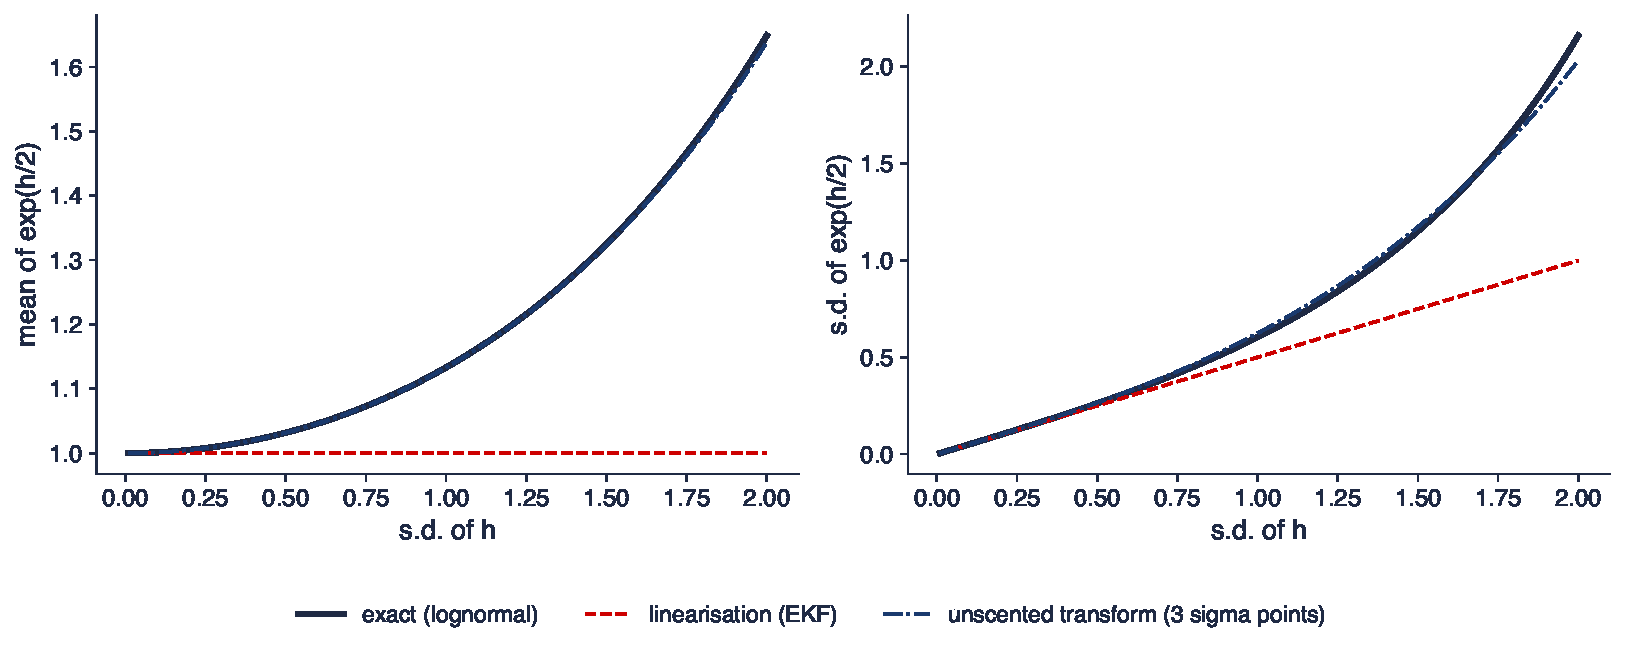
\includegraphics[width=0.97\textwidth,height=0.65\textheight,keepaspectratio]{ats_ch6_ukf.pdf}
\end{center}
\vspace{-0.25cm}
\begin{itemize}
    \item Volatilitatea din logaritmul varianței: media și abaterea standard a lui $\exp(h/2)$ pentru $h \sim N(0, s^2)$; momentele lognormale exacte, liniarizarea de ordinul întîi (EKF) și transformarea unscented cu trei puncte sigma
\end{itemize}
\quantlet{ATS\_ch6\_nonlinear\_filters}{\qlurl{ATS_ch6_nonlinear_filters}}
\end{frame}

\begin{frame}{Interpretarea transformării unscented}
\itemsize{\small}
\begin{itemize}
    \item Pentru $s = 1$: media exactă 1{,}131, liniarizarea 1{,}000, unscented 1{,}131; abaterea standard exactă 0{,}598, liniarizarea 0{,}496, unscented 0{,}618
    \item Liniarizarea ignoră convexitatea funcției $\exp$: subestimează volatilitatea așteptată, cu atît mai mult cu cît $h$ este mai incert
    \item Trei puncte sigma surprind convexitatea aproape exact pentru medie; varianța se abate pentru valori mari ale lui $s$
    \item Aceeași deplasare apare în practică: o prognoză EKF a volatilității sau a prețului unei opțiuni este prea mică atunci cînd starea este incertă
\end{itemize}
\end{frame}

\begin{frame}{Filtre de particule}
\itemsize{\footnotesize}
\begin{columns}[T]
\begin{column}{0.3\textwidth}
\centering
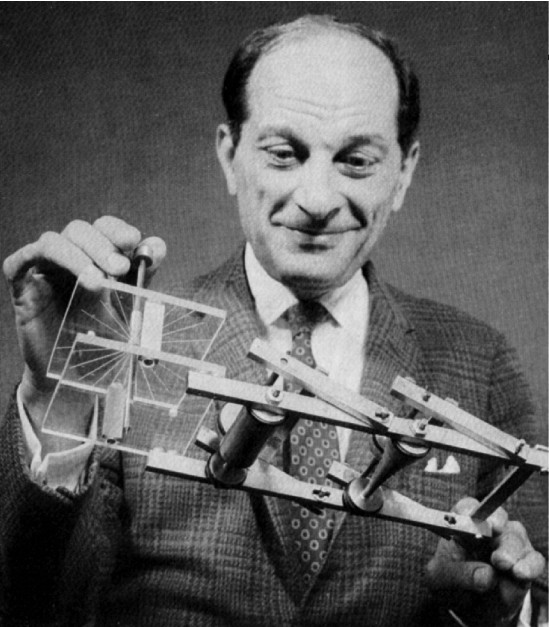
\includegraphics[height=0.32\textheight]{ch6_ulam_fermiac.jpg}\\[1mm]
\imgcap{Stanisław Ulam cu FERMIAC, un dispozitiv Monte Carlo}
\imgcredit{https://commons.wikimedia.org/wiki/File:STAN_ULAM_HOLDING_THE_FERMIAC.jpg}{Foto: Los Alamos National Laboratory (LA-UR-00-2532); public domain; Wikimedia Commons}
\end{column}
\begin{column}{0.68\textwidth}
\begin{itemize}
    \item Reprezentăm $p(x_t | Y_t)$ prin particule $x^{(i)}_t$ cu ponderi $W^{(i)}_t$, $i = 1, \dots, N$; metoda Monte Carlo provine de la Ulam și Metropolis (1949)
    \item Filtrul bootstrap \refGSS, \refKit
    \begin{itemize}
        \item propagăm: $x^{(i)}_t \sim f(\cdot | x^{(i)}_{t-1})$
        \item ponderăm: $w^{(i)}_t = g(y_t | x^{(i)}_t)$
        \item reeșantionăm $N$ particule cu probabilitățile $W^{(i)}_t \propto w^{(i)}_t$
    \end{itemize}
    \item Fără reeșantionare ponderile degenerează (o singură particulă preia toată ponderea); mărimea efectivă a eșantionului $\mathrm{ESS}_t = 1/\sum_i(W^{(i)}_t)^2$
    \item Reeșantionarea sistematică: o singură variabilă uniformă $U$, punctele $(U + i - 1)/N$ pe ponderile cumulate: varianță mai mică decît reeșantionarea multinomială
\end{itemize}
\end{column}
\end{columns}
\end{frame}

\begin{frame}{Verosimilitatea din filtrul de particule}
\itemsize{\small}
\begin{itemize}
    \item $\hat p(y_t | Y_{t-1}) = \frac1N\sum_i w^{(i)}_t$ și $\hat L(\psi) = \prod_t\hat p(y_t | Y_{t-1})$
    \item $\E\hat L(\psi) = L(\psi)$ exact, pentru orice $N \ge 1$ \refDM{} (\atsapplink{atsapp3}{atssrc3}{Anexa})  % applink: nedeplasarea verosimilității
    \begin{itemize}
        \item $\hat L$ este nedeplasat pe scala nivelului
        \item nu și pe scala logaritmică: dacă $\ln\hat L \approx N(\ln L - \tau^2/2, \tau^2)$, atunci $\E\ln\hat L = \ln L - \tau^2/2$; $\tau^2 = \Var\ln\hat L$
    \end{itemize}
    \item $\Var\ln\hat L$ crește aproximativ liniar în $n$ și scade ca $1/N$: un eșantion de două ori mai lung cere de două ori mai multe particule
    \item $\hat L(\psi)$ nu este netedă în $\psi$ (reeșantionarea este discontinuă): nu o maximizați prin metode de gradient; folosiți-o într-un MCMC
\end{itemize}
\end{frame}

\begin{frame}{Filtrul de particule pentru modelul SV al S\&P 500}
\itemsize{\footnotesize}
\begin{center}
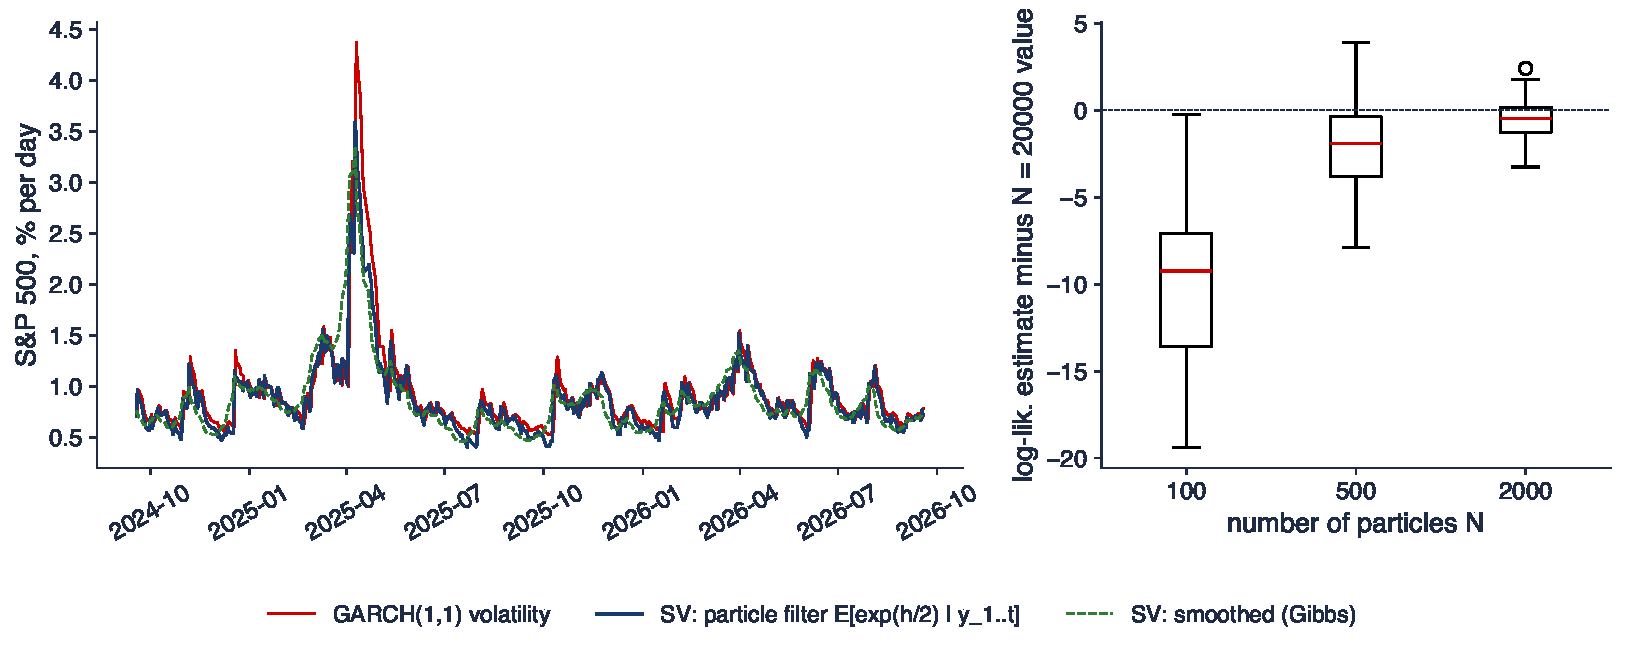
\includegraphics[width=0.97\textwidth,height=0.61\textheight,keepaspectratio]{ats_ch6_pf.pdf}
\end{center}
\vspace{-0.25cm}
\begin{itemize}
    \item Stînga: volatilitatea filtrată $\E[\exp(h_t/2) | Y_t]$ (filtrul bootstrap, $N = 20\,000$, media a posteriori Gibbs pentru $\psi$) față de GARCH(1,1) și traiectoria SV netezită, ultimii doi ani; dreapta: estimații ale log-verosimilității, cîte 100 de rulări pentru fiecare $N$
\end{itemize}
\quantlet{ATS\_ch6\_stochastic\_volatility}{\qlurl{ATS_ch6_stochastic_volatility}}
\end{frame}

\begin{frame}{Interpretarea filtrului de particule}
\itemsize{\footnotesize}
\begin{itemize}
    \item Abaterea standard Monte Carlo a lui $\ln\hat L$: 4{,}19 ($N = 100$), 2{,}38 ($N = 500$), 1{,}14 ($N = 2000$); un $N$ mic deplasează și $\ln\hat L$ în jos
    \item Log-verosimilitatea SV \ensuremath{-}3378{,}8 față de maximul GARCH(1,1) \ensuremath{-}3467{,}3: o diferență de 88{,}5 cu același număr de parametri
    \item Comparația favorizează SV chiar și la media a posteriori (nu la maximul) verosimilității sale; \refKSC\ compară SV cu modelele ARCH pe aceeași scală a verosimilității
    \item Volatilitatea SV filtrată este o estimație unilaterală, ca GARCH: corelația 0{,}96; traiectoria netezită anticipează punctele de întoarcere pentru că folosește date viitoare
    \item Mărimea efectivă a eșantionului pe parcursul eșantionului: minimum 150, mediana 18719 din 20\,000 de particule
\end{itemize}
\end{frame}

\begin{frame}{Filtrul de particule auxiliar}
\itemsize{\small}
\begin{itemize}
    \item Slăbiciunea filtrului bootstrap: particulele sînt propagate fără a ține cont de $y_t$; o valoare extremă lasă puține particule cu pondere
    \item APF \refPS: privim înainte de propagare
    \begin{itemize}
        \item prima etapă: reeșantionăm $x^{(i)}_{t-1}$ cu ponderi $\propto W^{(i)}_{t-1}\,g(y_t | \mu^{(i)}_t)$, $\mu^{(i)}_t = \E(x_t | x^{(i)}_{t-1})$
        \item a doua etapă: propagăm, apoi ponderăm cu $g(y_t | x^{(i)}_t)/g(y_t | \mu^{(k_i)}_t)$ pentru a corecta privirea înainte
        \item $k_i$: indicele particulei alese în prima etapă
    \end{itemize}
    \item Cazul complet adaptat: ponderi în prima etapă $p(y_t | x_{t-1})$ și propunerea $p(x_t | x_{t-1}, y_t)$: ponderile din etapa a doua sînt egale (optim local)
    \item Estimația verosimilității rămîne nedeplasată: $\hat p(y_t | Y_{t-1}) = \big(\sum_iW^{(i)}_{t-1}g(y_t | \mu^{(i)}_t)\big)\cdot\frac1N\sum_i\omega^{(i)}_t$; $\omega^{(i)}_t$: ponderile din etapa a doua
\end{itemize}
\end{frame}

\begin{frame}{Verosimilitățile din filtrele de particule față de verosimilitatea Kalman exactă}
\itemsize{\footnotesize}
\begin{center}
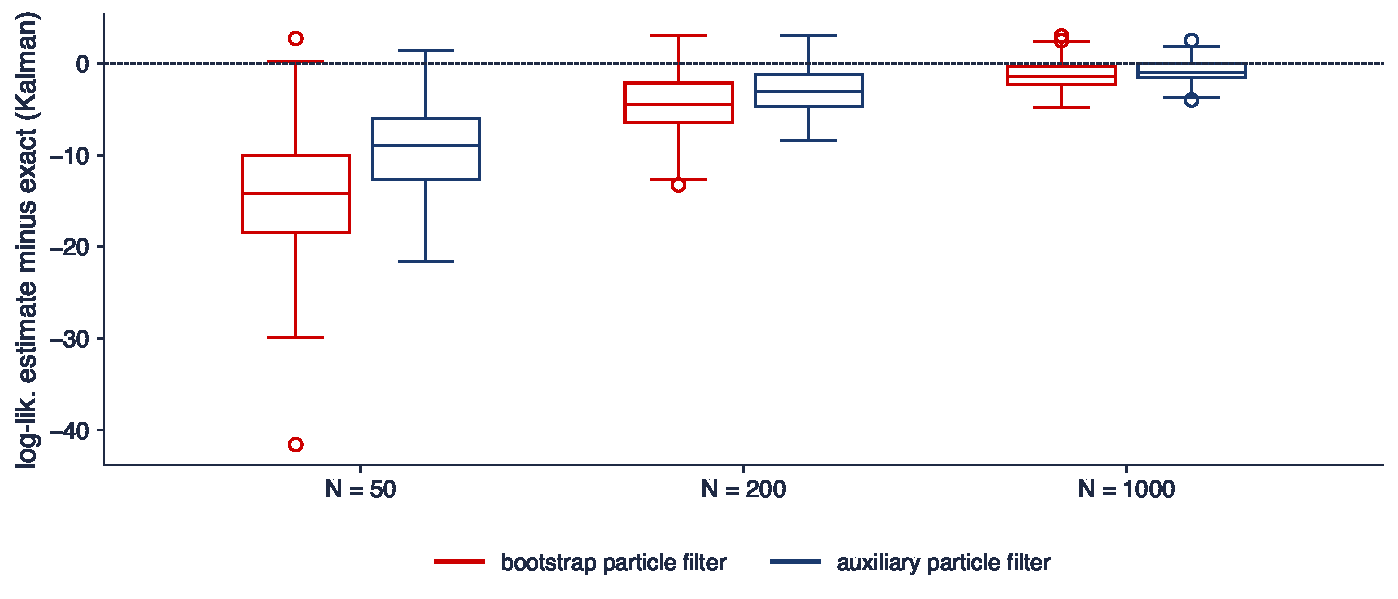
\includegraphics[width=0.97\textwidth,height=0.65\textheight,keepaspectratio]{ats_ch6_pf_check.pdf}
\end{center}
\vspace{-0.25cm}
\begin{itemize}
    \item Modelul local level pentru inflația din SUA, la varianțele ML: eroarea lui $\ln\hat L$ (condiționat de $y_1$) pentru filtrul bootstrap și pentru cel auxiliar, cîte 200 de rulări pentru fiecare $N$
\end{itemize}
\quantlet{ATS\_ch6\_nonlinear\_filters}{\qlurl{ATS_ch6_nonlinear_filters}}
\end{frame}

\begin{frame}{Interpretarea verificării filtrelor de particule}
\itemsize{\small}
\begin{itemize}
    \item Eroarea medie a lui $\ln\hat L$: \ensuremath{-}14{,}37; \ensuremath{-}4{,}48; \ensuremath{-}1{,}30 (bootstrap, $N = 50, 200, 1000$) și \ensuremath{-}9{,}37; \ensuremath{-}2{,}87; \ensuremath{-}0{,}88 (auxiliar)
    \item Abaterile standard: 1{,}46 (bootstrap) și 1{,}17 (auxiliar) pentru $N = 1000$: privirea înainte crește precizia, pentru că raportul semnal--zgomot este mare
    \item Media negativă este deplasarea Jensen a logaritmului unui estimator nedeplasat: scade ca $\Var(\ln\hat L)/2$
    \item Testați întotdeauna un filtru de particule pe un model cu verosimilitate cunoscută înainte de a-l folosi acolo unde aceasta nu este disponibilă
\end{itemize}
\end{frame}

\begin{frame}{Particle MCMC}
\itemsize{\small}
\begin{itemize}
    \item Ideea pseudo-marginală \refAR: rulăm Metropolis--Hastings cu o estimație nedeplasată și pozitivă $\hat L(\psi)$ în locul lui $L(\psi)$; lanțul are ca țintă tot distribuția a posteriori exactă $p(\psi | Y_n)$
    \item PMMH \refADH
    \begin{itemize}
        \item propunem $\psi'$ din densitatea de propunere $q(\cdot | \psi)$; rulăm un filtru de particule pentru $\hat L(\psi')$
        \item acceptăm cu probabilitatea $\min\{1, \hat L(\psi')p(\psi')q(\psi | \psi') / [\hat L(\psi)p(\psi)q(\psi' | \psi)]\}$; $p(\cdot)$: distribuția a priori
        \item păstrăm $\hat L$ al punctului curent (nu îl recalculăm)
    \end{itemize}
    \item Alegerea lui $N$ \refPSGK, \refDPDK
    \begin{itemize}
        \item prea puține particule blochează lanțul; prea multe irosesc timpul
        \item ținta: $\Var(\ln\hat L) \approx 1$--$2$ la media a posteriori
        \item particle Gibbs (SMC condiționat) eșantionează și traiectoria stării; util atunci cînd nu există o structură condiționat gaussiană
    \end{itemize}
    \item Funcționează pentru orice model pe care îl puteți simula și a cărui densitate de măsurare o puteți evalua: SV cu salturi, modele DSGE, modele UC neliniare
\end{itemize}
\end{frame}

\begin{frame}{PMMH față de eșantionatorul Gibbs KSC}
\itemsize{\footnotesize}
\begin{center}
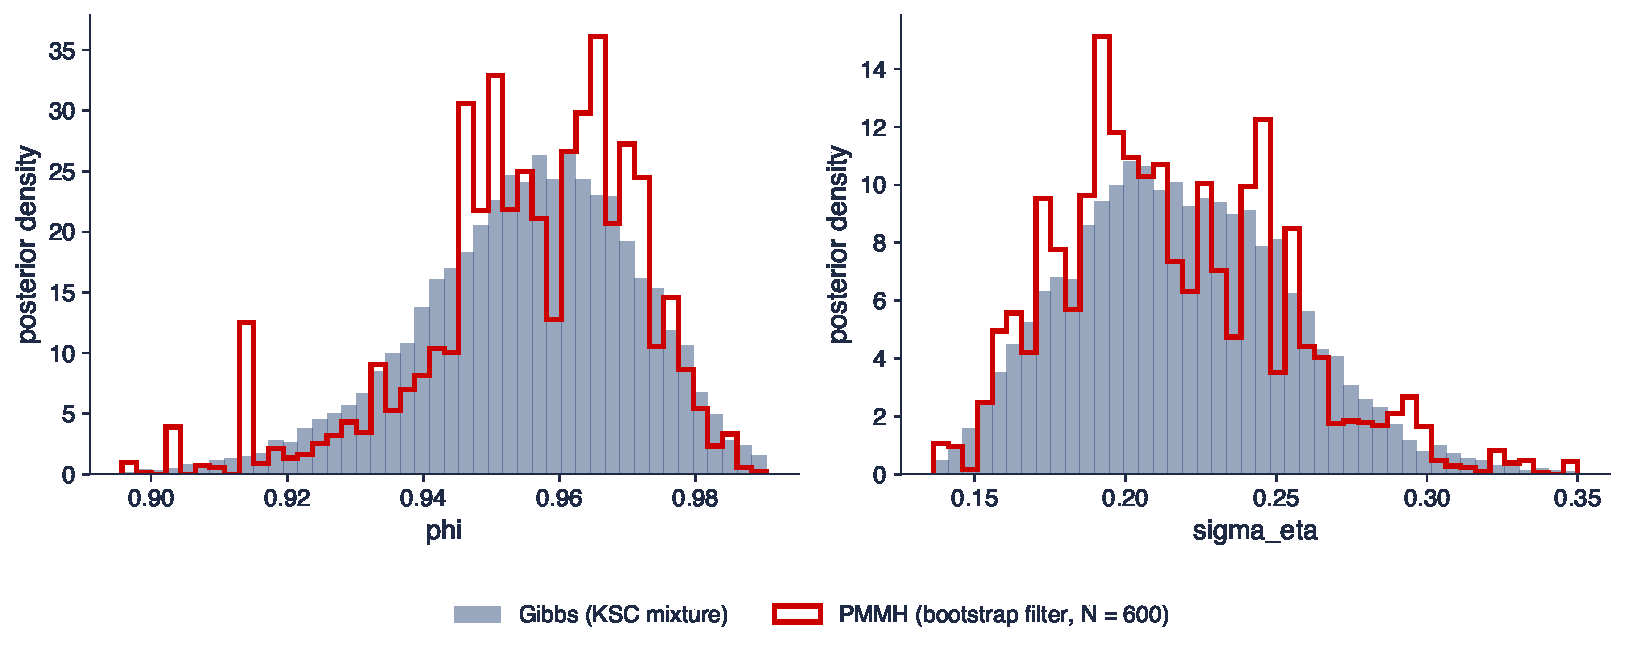
\includegraphics[width=0.97\textwidth,height=0.65\textheight,keepaspectratio]{ats_ch6_pmmh.pdf}
\end{center}
\vspace{-0.25cm}
\begin{itemize}
    \item Ultimele 1000 de randamente S\&P 500; PMMH cu un filtru bootstrap de $N = 600$ particule, 10\,000 de iterații, mers aleator pe $(\mu, \operatorname{atanh}\phi, \ln\sigma_\eta)$; Gibbs cu mixtura KSC
\end{itemize}
\quantlet{ATS\_ch6\_stochastic\_volatility}{\qlurl{ATS_ch6_stochastic_volatility}}
\end{frame}

\begin{frame}{Interpretarea rulării PMMH}
\itemsize{\small}
\begin{itemize}
    \item Mediile a posteriori ale lui $\phi$: 0{,}955 (Gibbs) și 0{,}955 (PMMH); ale lui $\sigma_\eta$: 0{,}219 și 0{,}216; abaterile standard a posteriori 0{,}037 și 0{,}039
    \item Doi algoritmi exacți, aceeași distribuție a posteriori: aproximarea prin mixtura KSC nu are aici un efect vizibil
    \item $N = 600$ dă o abatere standard a lui $\ln\hat L$ de 1{,}19 la media a posteriori, în intervalul recomandat; rata de acceptare este 13\%
    \item Costul: 3{,}6 minute pentru PMMH, față de cîteva secunde pentru Gibbs: folosiți PMMH cînd nu există o reprezentare condiționat gaussiană
\end{itemize}
\end{frame}

\begin{frame}{Recapitulare: filtrarea neliniară}
\itemsize{\small}
\begin{itemize}
    \item EKF liniarizează modelul, UKF propagă puncte sigma, filtrele de particule propagă eșantioane ponderate
    \item Verosimilitatea din filtrul de particule este nedeplasată în nivel; varianța logaritmului ei decide numărul de particule
    \item PMMH transformă orice model care poate fi simulat într-o procedură bayesiană exactă, cu un cost de calcul
\end{itemize}
\end{frame}


%=============================================================================
\section{Parametri variabili în timp}
%=============================================================================

\begin{frame}{O regresie TVP în forma în spațiul stărilor}
\itemsize{\small}
\begin{itemize}
    \item $y_t = c_t + b_tx_t + D_t'\gamma + \varepsilon_t$, $\quad c_{t+1} = c_t + \eta_{c,t}$, $\quad b_{t+1} = b_t + \eta_{b,t}$
    \begin{itemize}
        \item $c_t$, $b_t$: termenul liber și panta, mersuri aleatoare cu varianțele $\sigma^2_c$, $\sigma^2_b$; $D_t$: variabile dummy cu $\gamma$ fix
        \item starea $\alpha_t = (c_t, b_t, \gamma')'$; $Z_t = (1, x_t, D_t')$
    \end{itemize}
    \item Coeficienții ficși ($\gamma$, aici variabile dummy sezoniere trimestriale) sînt stări cu varianță zero și start difuz: $d$ = numărul stărilor = 5
    \begin{itemize}
        \item cu $\sigma^2_c = \sigma^2_b = 0$, netezitorul dă estimațiile OLS (cele mai mici pătrate recursive)
    \end{itemize}
    \item Întrebarea: s-a schimbat co-mișcarea inflației din România cu inflația din zona euro de la introducerea țintirii inflației (2005)?
    \item $y_t$: inflația IAPC din România, trimestrial, \% anualizat, neajustată sezonier; $x_t$: inflația IAPC din zona euro fără componenta sezonieră; T4 2005--T2 2026, $T = 83$
    \item Testul pantei constante: $H_0$: $\sigma^2_b = 0$ pe frontieră; bootstrap parametric pentru statistica LR din modelul restricționat (199 de eșantioane)
\end{itemize}
\end{frame}

\begin{frame}{Inflația din România și inflația din zona euro: o pantă variabilă în timp?}
\itemsize{\footnotesize}
\begin{center}
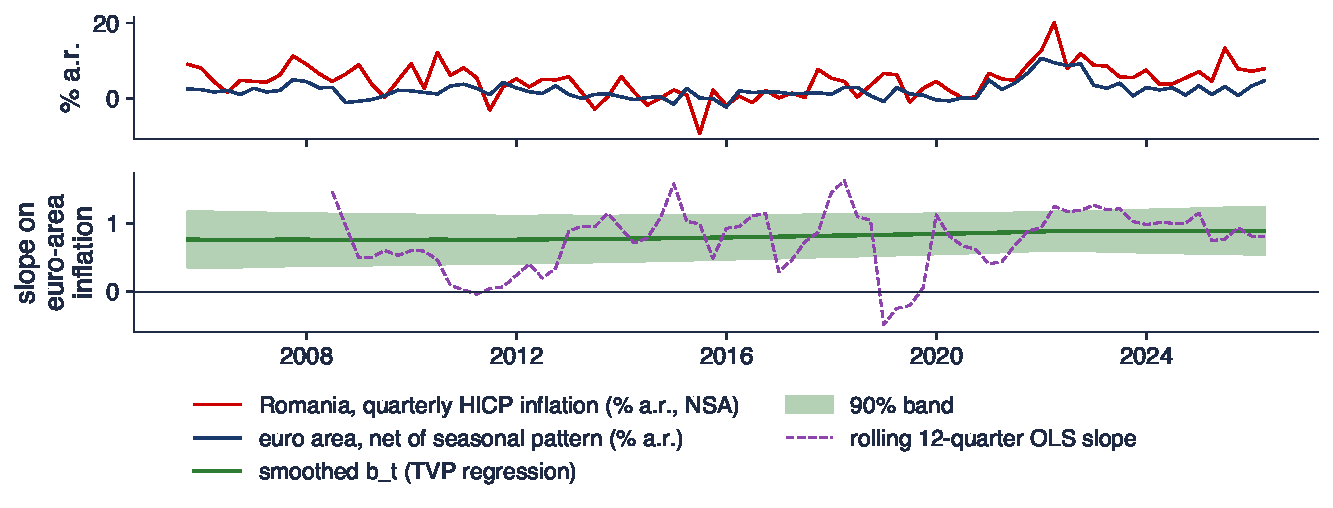
\includegraphics[width=0.97\textwidth,height=0.65\textheight,keepaspectratio]{ats_ch6_tvp.pdf}
\end{center}
\vspace{-0.25cm}
\begin{itemize}
    \item Sus: cele două rate ale inflației; jos: $b_t$ netezit cu o bandă de 90\% (ML difuz exact) și panta unei regresii mobile pe 12 trimestre cu aceleași variabile dummy
\end{itemize}
\quantlet{ATS\_ch6\_tvp\_inflation}{\qlurl{ATS_ch6_tvp_inflation}}
\end{frame}

\begin{frame}{Interpretarea regresiei TVP}
\itemsize{\small}
\begin{itemize}
    \item ML: $\hat\sigma^2_c = 0{,}332$, $\hat\sigma^2_b = 0{,}0011$, $\hat\sigma^2_\varepsilon = 7{,}21$; log-verosimilitățile numpy și \texttt{statsmodels} sînt \ensuremath{-}209{,}93 și \ensuremath{-}209{,}93
    \item $b_t$ se deplasează de la 0{,}76 (eroare standard 0{,}23) în T3 2008 la 0{,}89 (eroare standard 0{,}17) în T4 2022: o pantă apropiată de unu, dar fără o schimbare semnificativă
    \item LR $= 0{,}066$; p-value-ul bootstrap $= 0{,}265$ (cuantila de 95\% este 1{,}91; 66\% dintre statisticile bootstrap sînt exact zero: din nou pile-up); regula $\frac12\chi^2_1$ dă $p = 0{,}399$
    \item Regresia mobilă oscilează între valori negative și 1,5: acesta este zgomotul de eșantionare al ferestrelor de 12 trimestre, nu variație în timp; modelul în spațiul stărilor îl mediază printr-o varianță explicită
\end{itemize}
\end{frame}

\begin{frame}{TVP-VAR cu volatilitate stochastică}
\itemsize{\footnotesize}
\begin{columns}[T]
\begin{column}{0.3\textwidth}
\centering
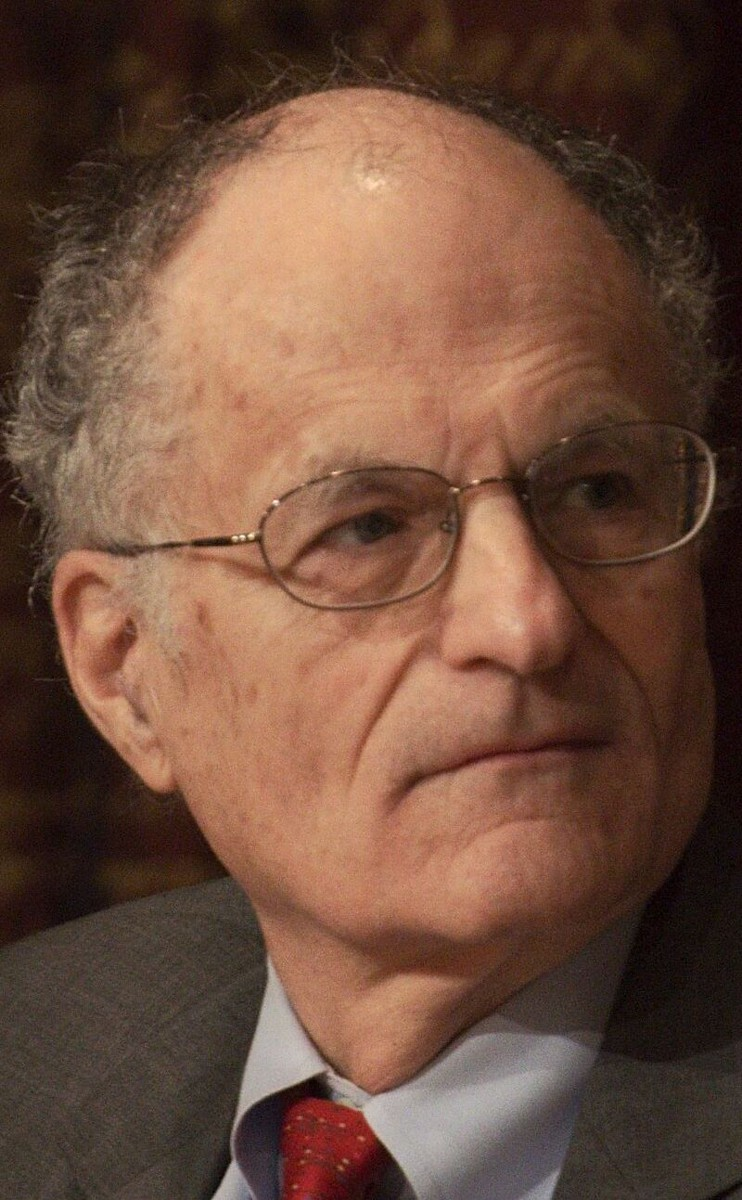
\includegraphics[height=0.36\textheight]{ch6_sargent_2011.jpg}\\[1mm]
\imgcap{Thomas J. Sargent, 2011}
\imgcredit{https://commons.wikimedia.org/wiki/File:Thomas_J._Sargent_close-up_(cropped).jpg}{Foto: Holger Motzkau (2011); CC BY-SA 3.0; Wikimedia Commons}
\end{column}
\begin{column}{0.68\textwidth}
\begin{itemize}
    \item \refCSa, \refCSb, \refPri: $y_t = X_t'\beta_t + A_t^{-1}\Sigma_t\epsilon_t$
    \begin{itemize}
        \item $X_t$: lagurile; $\beta_t$: coeficienții; $\epsilon_t \sim N(0, I)$
        \item $A_t$: inferior triunghiulară, cu elementele libere $a_t$; $\Sigma_t = \mathrm{diag}(\sigma_{j,t})$
        \item $\beta_t$, $a_t$ și $\ln\sigma_{j,t}$ urmează mersuri aleatoare
    \end{itemize}
    \item Întrebarea: s-a schimbat politica monetară a SUA (coeficienți care derivă) sau s-au micșorat șocurile (volatilități în scădere) după 1980?
    \item Răspunsul din \refPri: reacția sistematică a politicii monetare s-a schimbat, dar aceste schimbări explică puțin din anii 1970; varianța șocurilor care nu țin de politica monetară contează mai mult
    \item Fără volatilitate stochastică, scăderea varianțelor șocurilor este atribuită greșit schimbării coeficienților
\end{itemize}
\end{column}
\end{columns}
\end{frame}

\begin{frame}{Estimarea unui TVP-VAR-SV}
\itemsize{\small}
\begin{itemize}
    \item Blocurile Gibbs, fiecare fiind unul dintre eșantionatoarele din acest capitol:
    \begin{itemize}
        \item $\beta_{1:n}$ | rest: simulation smoother pentru un model liniar gaussian cu covarianțe cunoscute, variabile în timp
        \item $a_{1:n}$ | rest: ecuație cu ecuație, același netezitor
        \item $\ln\sigma_{j,1:n}$ | rest: mixtura KSC cu indicatorii ei
        \item covarianțele mersurilor aleatoare: invers Wishart
    \end{itemize}
    \item Ordinea pașilor Gibbs contează: algoritmul inițial extrăgea indicatorii mixturii într-un punct greșit al ciclului; \refDNP\ dau ordinea corectă, iar rezultatele de fond se schimbă puțin
    \item Distribuții a priori dintr-un eșantion de antrenare de la începutul datelor, ca în \refPri, cu scale mici pentru covarianțele mersurilor aleatoare: a priori decide cîtă variație este permisă
    \item Supraparametrizarea: cu $k$ coeficienți pe ecuație, aplicăm shrinkage varianțelor sau selectăm coeficienții care variază (parametrizarea necentrată, \refFSW)
\end{itemize}
\end{frame}

\begin{frame}{Recapitulare: parametri variabili în timp}
\itemsize{\small}
\begin{itemize}
    \item O regresie TVP este un model în spațiul stărilor cu $Z_t$ construit din regresori; coeficienții ficși sînt stări difuze fără șocuri
    \item Ferestrele mobile exagerează variația în timp; testați-o la frontieră cu un bootstrap
    \item TVP-VAR-SV combină simulation smoother-ul și mixtura KSC într-un singur eșantionator Gibbs
\end{itemize}
\end{frame}


%=============================================================================
\section{Modele cu factori dinamici în forma în spațiul stărilor}
%=============================================================================

\begin{frame}{DFM ca model în spațiul stărilor (1/2)}
\itemsize{\small}
\begin{itemize}
    \item $x_{it} = \lambda_i'f_t + e_{it}$, $\quad f_t = \Phi f_{t-1} + u_t$, $\quad e_{it} = \rho_ie_{i,t-1} + \nu_{it}$
    \begin{itemize}
        \item $f_t$: factorii, un VAR(1) cu matricea $\Phi$; $\lambda_i$: ponderile factoriale ale seriei $i$, așezate în $\Lambda$
        \item $e_{it}$: erori idiosincratice AR(1) cu coeficienții $\rho_i$; $u_t$, $\nu_{it}$: șocurile
        \item starea $(f_t', f_{t-1}', e_t')'$; matricea de măsurare $Z = (\Lambda, 0, I)$
    \end{itemize}
    \item Frecvențele mixte \refMM
    \begin{itemize}
        \item o rată de creștere trimestrială este o sumă ponderată a stărilor lunare
        \item filtrul sare pur și simplu peste lunile lipsă
    \end{itemize}
\end{itemize}
\end{frame}

\begin{frame}{DFM ca model în spațiul stărilor (2/2)}
\itemsize{\small}
\begin{itemize}
    \item Estimarea
    \begin{itemize}
        \item în doi pași \refDGR: componentele principale dau $\Lambda$, $\Phi$, $\Sigma_e$; apoi netezitorul Kalman reestimează $f_t$ pe panelul complet; consistent cînd $N, T \to \infty$
        \item ML prin EM \refSS, \refBM: pasul E este netezitorul, sînt permise structuri arbitrare de date lipsă
        \item $N$ mare: comprimăm cele $N$ observații într-un vector de dimensiune $r$ înainte de filtrare \refJK; costul nu mai crește ca $N^3$
    \end{itemize}
    \item Nowcasting \refGRS: ragged edge, descompunerea pe știri și evaluarea în timp real se află în \atschlink{https://danpele.github.io/Advanced-Time-Series/RO/Cursuri/capitol5_bvar_modele_factoriale_nowcasting.pdf}{Capitolul 5}; această secțiune arată mecanismul în spațiul stărilor
\end{itemize}
\end{frame}

\begin{frame}{Un model cu un factor pentru indicatorii coincidenți ai SUA}
\itemsize{\footnotesize}
\begin{center}
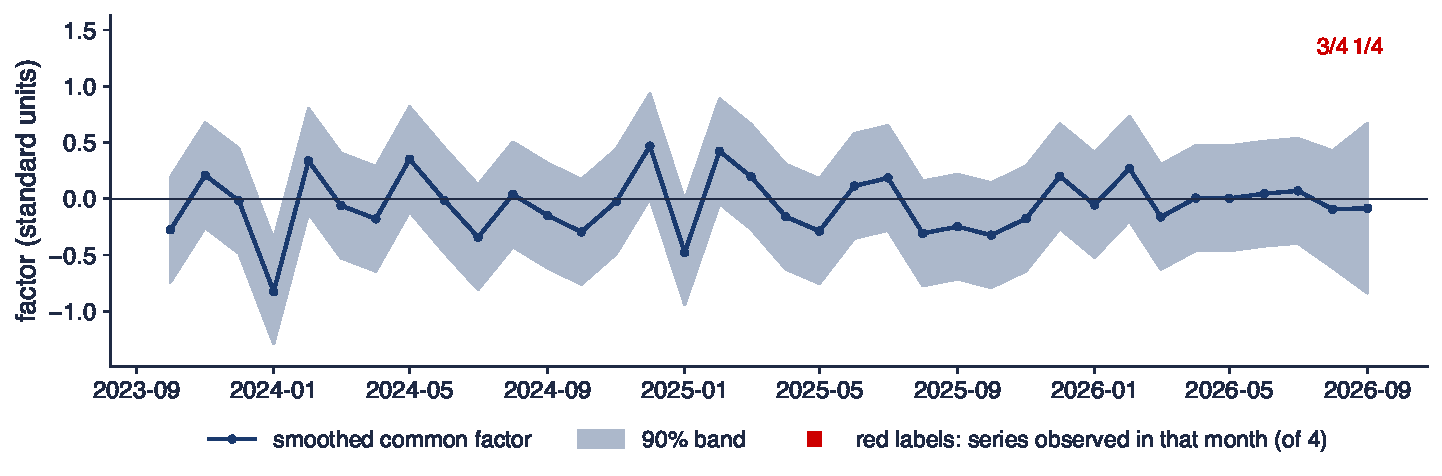
\includegraphics[width=0.97\textwidth,height=0.61\textheight,keepaspectratio]{ats_ch6_dfm.pdf}
\end{center}
\vspace{-0.25cm}
\begin{itemize}
    \item Creșterea lunară a producției industriale, a numărului de salariați, a venitului real fără transferuri și a vînzărilor reale (FRED), standardizate, ianuarie 1990--septembrie 2026; estimatorul în doi pași, tratarea univariată a vectorului de observații; ultimele 36 de luni
\end{itemize}
\quantlet{ATS\_ch6\_dfm\_ragged\_edge}{\qlurl{ATS_ch6_dfm_ragged_edge}}
\end{frame}

\begin{frame}{Interpretarea datelor incomplete la sfîrșitul eșantionului (ragged edge)}
\itemsize{\small}
\begin{itemize}
    \item Încărcările factoriale 0{,}90; 0{,}89; 0{,}68; 0{,}84; coeficientul AR al factorului 0{,}12: ratele lunare de creștere sînt puțin persistente, deci factorul este în principal o medie ponderată a lunii
    \item Ultima lună completă este iulie 2026: abaterea standard a factorului este 0{,}28; în septembrie 2026, cu o singură serie din patru disponibilă, crește la 0{,}46
    \item Filtrul ponderează fiecare serie după raportul ei semnal--zgomot; nicio serie nu este eliminată, niciun gol nu este completat de mînă
    \item Prognoza factorului dincolo de date este aceeași recursie, cu toate observațiile lipsă
\end{itemize}
\end{frame}


%=============================================================================
\section{Descompuneri trend--ciclu, revizitate}
%=============================================================================

\begin{frame}{Trei definiții ale ciclului}
\itemsize{\small}
\begin{itemize}
    \item Beveridge--Nelson \refBN: trendul = prognoza pe orizont lung fără drift
    \begin{itemize}
        \item $\tau^{BN}_t = y_t + \sum_{j\ge1}\E_t(\Delta y_{t+j} - \mu)$; ciclul $c^{BN}_t = y_t - \tau^{BN}_t$
        \item $\E_t$: speranța condiționată de datele pînă la $t$; $\mu$: creșterea medie; trendul este nivelul la care se așteaptă să ajungă $y$ după ce creșterea previzibilă s-a stins
        \item pentru un AR(1) în creștere: $c^{BN}_t = -\frac{\phi}{1 - \phi}(\Delta y_t - \mu)$; unilateral, depinde de modelul ARMA ales; versiuni fiabile: \refKMW
    \end{itemize}
    \item Componente neobservate \refCla, \refWat, \refHJ: $y_t = \tau_t + c_t$, cu trend mers aleator (sau neted) și ciclu AR(2); bilateral după netezire
    \item Hamilton \refHamB: $c_{t+h}$ = reziduul regresiei lui $y_{t+h}$ pe $(1, y_t, \dots, y_{t-3})$, $h = 8$ trimestre; fără model și unilateral (\atschlink{https://danpele.github.io/Time-Series-Analysis/RO/Cursuri/capitol10_spatiul_starilor_kalman_markov_switching.pdf}{TSA, Capitolul 10})
    \item Pentru PIB-ul SUA ciclul BN este mic și zgomotos, ciclul UC mare și neted: aceleași date, două povești. De ce?
\end{itemize}
\end{frame}

\begin{frame}{Componente neobservate cu șocuri corelate}
\itemsize{\small}
\begin{itemize}
    \item \refMNZ, modelul UC-UR
    \begin{itemize}
        \item $y_t = \tau_t + c_t$, $\tau_t = \mu + \tau_{t-1} + \eta_t$, $c_t = \phi_1c_{t-1} + \phi_2c_{t-2} + \varepsilon_t$, $\Corr(\eta_t, \varepsilon_t) = \rho$
        \item $\tau_t$: trendul stochastic cu driftul $\mu$ și șocurile $\eta_t$ (abaterea standard $\sigma_\eta$); $c_t$: un ciclu AR(2) cu șocurile $\varepsilon_t$ (abaterea standard $\sigma_\varepsilon$); $\rho$: corelația celor două șocuri
    \end{itemize}
    \item Modelul UC0 al lui Clark impune $\rho = 0$; cu un ciclu AR(2), $\rho$ este identificat: forma redusă este un ARIMA(2,1,2), cu tot atîția parametri cît UC-UR
    \begin{itemize}
        \item cu un ciclu AR(1), $\rho$ nu este identificat
    \end{itemize}
    \item Rezultatul: dacă $\rho$ este liber, ciclul UC filtrat coincide cu ciclul BN al modelului ARIMA(2,1,2): diferența dintre BN și UC era restricția $\rho = 0$
    \item Starea $(\tau_t, c_t, c_{t-1})$: $\tau$ difuz, blocul ciclului staționar (inițializare mixtă); studiul de caz de mai jos: eșantionul lor, T1 1947--T2 1998, datele din ediția actuală
\end{itemize}
\end{frame}

\begin{frame}{Replicarea Morley, Nelson și Zivot (2003)}
\itemsize{\footnotesize}
\begin{center}
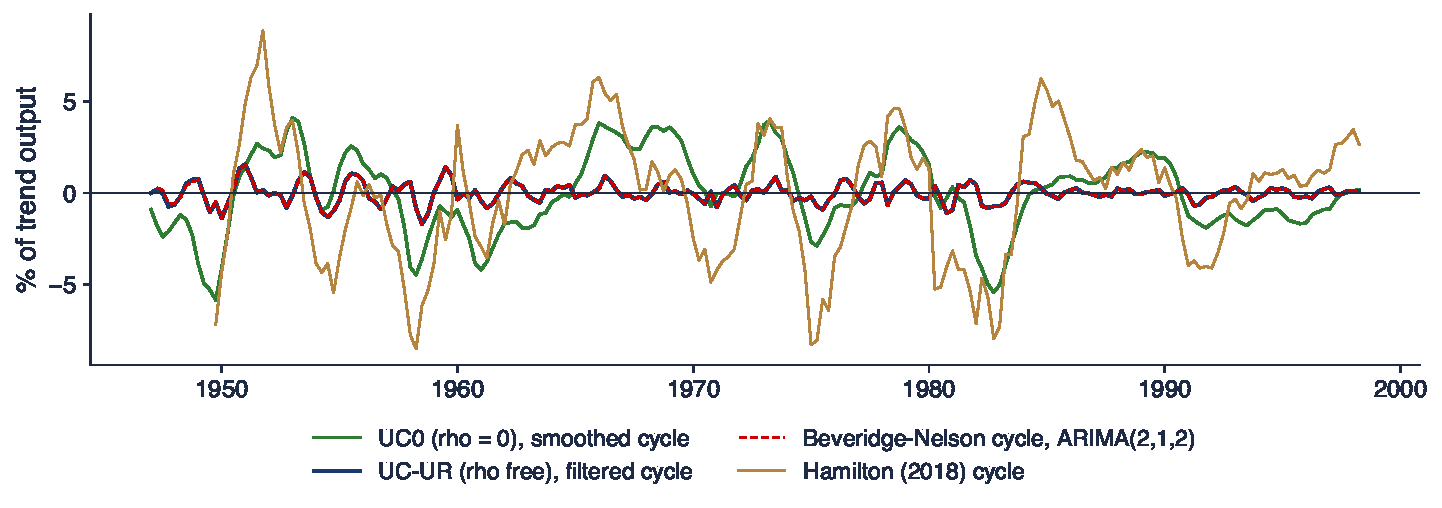
\includegraphics[width=0.97\textwidth,height=0.65\textheight,keepaspectratio]{ats_ch6_mnz.pdf}
\end{center}
\vspace{-0.25cm}
\begin{itemize}
    \item 100$\times$log PIB real al SUA (FRED GDPC1), $T = 206$; UC0 și UC-UR prin ML difuz exact; ciclul BN dintr-un ARIMA(2,1,2); ciclul Hamilton (2018) pentru comparație
\end{itemize}
\quantlet{ATS\_ch6\_trend\_cycle}{\qlurl{ATS_ch6_trend_cycle}}
\end{frame}

\begin{frame}{Interpretarea replicării MNZ}
\itemsize{\footnotesize}
\begin{center}
\footnotesize
\begin{tabular}{lccccccc}
\toprule
Model & $\mu$ & $\phi_1$ & $\phi_2$ & $\sigma_\eta$ & $\sigma_\varepsilon$ & $\rho$ & $\ln L$ \\
\midrule
UC0 & 0{,}858 & 1{,}501 & \ensuremath{-}0{,}571 & 0{,}612 & 0{,}665 & 0 & \ensuremath{-}280{,}81 \\
UC-UR & 0{,}859 & 1{,}334 & \ensuremath{-}0{,}738 & 1{,}185 & 0{,}669 & \ensuremath{-}0{,}927 & \ensuremath{-}279{,}35 \\
\bottomrule
\end{tabular}
\end{center}
\begin{itemize}
    \item $\hat\rho = \ensuremath{-}0{,}927$: șocurile trendului și ale ciclului sînt corelate negativ aproape perfect; șocurile trendului sînt mai mari decît cele ale ciclului ($\hat\sigma_\eta > \hat\sigma_\varepsilon$)
    \item Corelația ciclului UC-UR filtrat cu ciclul BN (coeficienții AR ai ARIMA 1{,}334; \ensuremath{-}0{,}738, ca în UC-UR): 0{,}999; abaterile standard ale ciclurilor: UC0 2{,}20, UC-UR 0{,}52, BN 0{,}52, Hamilton 3{,}50
    \item Testul LR pentru $\rho = 0$: 2{,}92, $p = 0{,}088$ ($\chi^2_1$); ciclul UC0 este mare pentru că este presupus ortogonal pe trend, nu pentru că datele o cer
    \item Cifrele noastre folosesc ediția actuală a datelor PIB; estimațiile din lucrare diferă la zecimale, nu în concluzie
\end{itemize}
\end{frame}

\begin{frame}{România: ciclul este trendul}
\itemsize{\footnotesize}
\begin{columns}[T]
\begin{column}{0.3\textwidth}
\centering
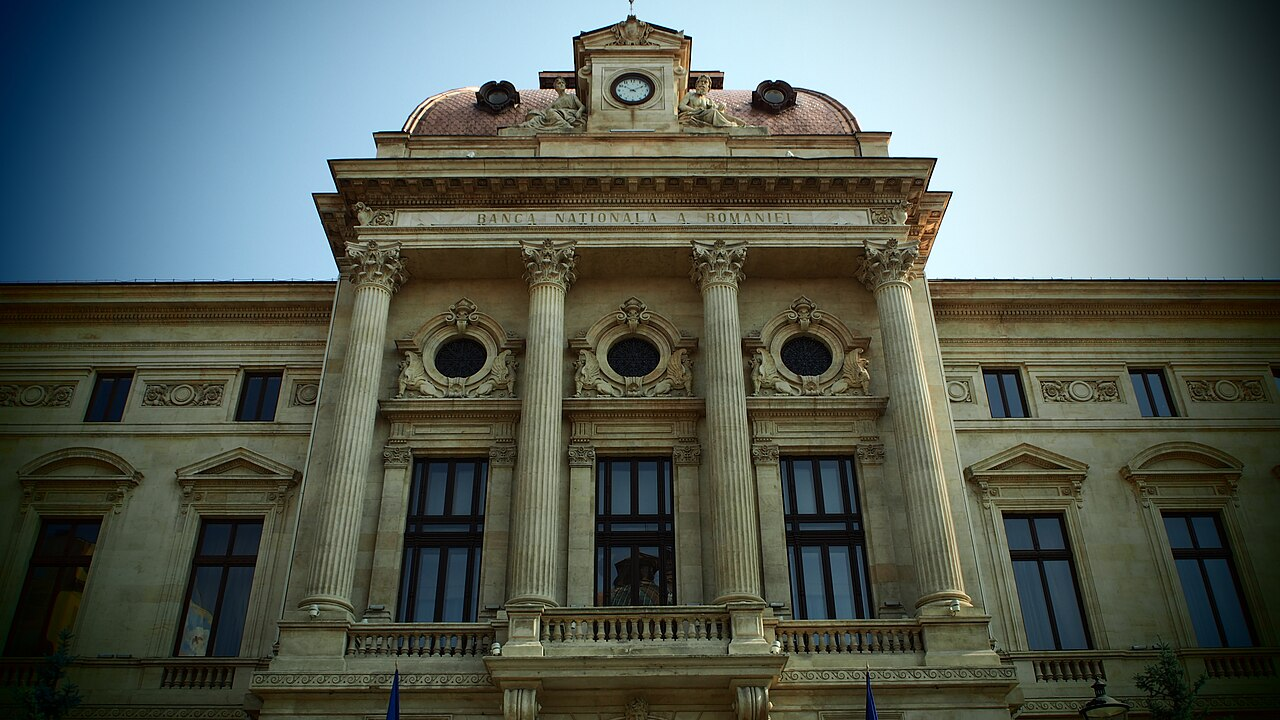
\includegraphics[height=0.30\textheight]{ch0_bnr_palace_2015.jpg}\\[1mm]
\imgcap{Palatul BNR, București}
\imgcredit{https://commons.wikimedia.org/wiki/File:Bucharest_-_BNR_Palace_(19644434340).jpg}{Foto: Ștefan Jurcă (2015); CC BY 2.0; Wikimedia Commons}
\end{column}
\begin{column}{0.68\textwidth}
\begin{itemize}
    \item Economiile emergente au șocuri de trend volatile \refAG: un trend de tip mers aleator absoarbe cea mai mare parte a mișcării PIB
    \item UC0 pentru România, T1 2000--T2 2026 (T2--T4 2020 tratate ca lipsă): $\hat\sigma_\eta = 1{,}897$, $\hat\sigma_\varepsilon = 0{,}950$, $\hat\phi_1 = 0{,}280$, $\hat\phi_2 = \ensuremath{-}0{,}261$: un ciclu scurt și slab
    \item UC-UR: $\hat\rho = 1{,}00$ la frontieră, LR $= 2{,}92$: în 106 trimestre corelația este slab determinată
    \item Alternativa: un trend neted (mers aleator integrat, modelul HP \refHJ) cu un ciclu AR(2): $\hat\sigma^2_\zeta = 0{,}0046$, $\hat\sigma^2_\varepsilon = 4{,}95$, $\hat\phi = (0{,}87; 0{,}09)$
\end{itemize}
\end{column}
\end{columns}
\end{frame}

\begin{frame}{Output gap-ul României}
\itemsize{\footnotesize}
\begin{center}
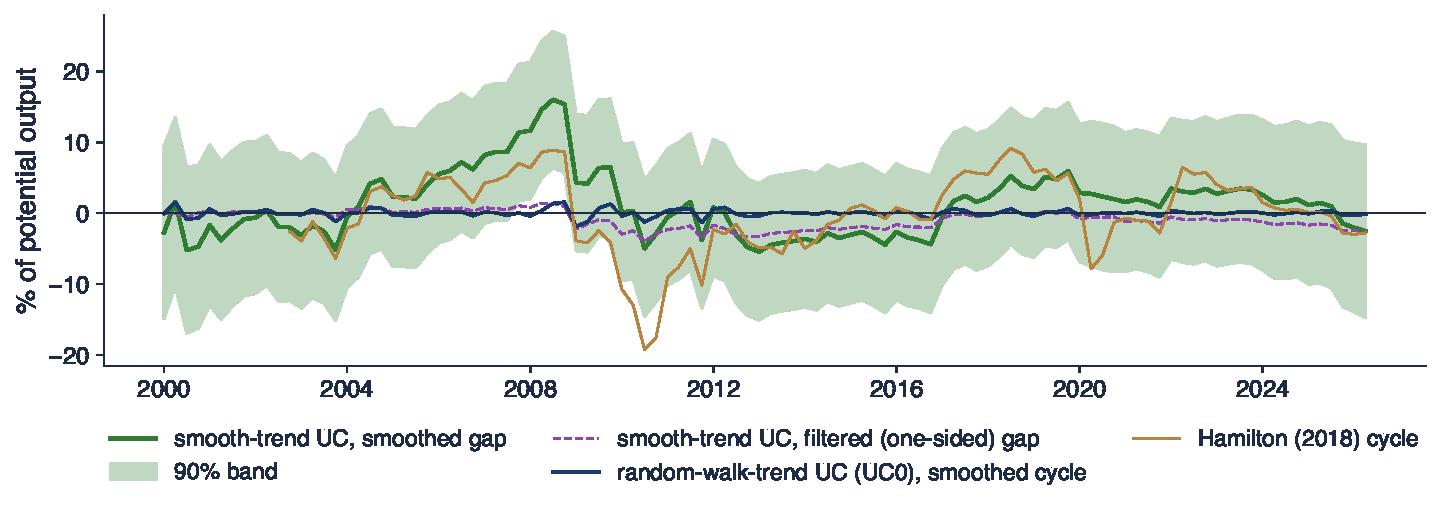
\includegraphics[width=0.97\textwidth,height=0.65\textheight,keepaspectratio]{ats_ch6_ro_gap.pdf}
\end{center}
\vspace{-0.25cm}
\begin{itemize}
    \item 100$\times$log PIB real, Eurostat, ajustat sezonier și cu numărul de zile lucrătoare; UC cu trend neted (netezit, cu bandă de 90\%, și filtrat), UC0 cu trend mers aleator, Hamilton (2018) pe seria completă
\end{itemize}
\quantlet{ATS\_ch6\_trend\_cycle}{\qlurl{ATS_ch6_trend_cycle}}
\end{frame}

\begin{frame}{Interpretarea output gap-ului României}
\itemsize{\small}
\begin{itemize}
    \item Output gap-ul cu trend neted: 16{,}0\% în T3 2008 (abatere standard 5{,}9), \ensuremath{-}5{,}0\% în T3 2010, 5{,}9\% în T4 2019; ultimul trimestru \ensuremath{-}2{,}6\% (abatere standard 7{,}4)
    \item În timp real situația este alta: output gap-ul filtrat era doar 1{,}4\% în T3 2008 și 0{,}3\% în T4 2019; abaterea standard a revizuirilor (netezit minus filtrat): 3{,}8 pp \refOvN
    \item Alegerea modelului domină: abaterea standard a output gap-ului este 4{,}5 (trend neted), 0{,}53 (UC0), 5{,}4 (Hamilton); corelația trend neted--Hamilton 0{,}65
    \item Un output gap pentru România fără banda lui și fără modelul din spatele lui nu este o informație
\end{itemize}
\end{frame}

\begin{frame}{Recapitulare: descompunerile trend--ciclu}
\itemsize{\small}
\begin{itemize}
    \item BN, UC și Hamilton definesc ciclul diferit; MNZ arată că BN și UC coincid odată ce șocurile trendului și ale ciclului pot fi corelate
    \item În eșantioane scurte și volatile (România) corelația nu este identificată, iar specificarea trendului decide output gap-ul
    \item Raportați estimațiile filtrate și netezite: output gap-ul de la finalul eșantionului este cifra cea mai puțin fiabilă
\end{itemize}
\end{frame}


%=============================================================================
\section{Inflația de trend cu volatilitate stochastică}
%=============================================================================

\begin{frame}{Modelul UC-SV al lui Stock și Watson (2007)}
\itemsize{\small}
\begin{itemize}
    \item $\pi_t = \tau_t + \sigma_{\eta,t}\eta_t$, $\quad \tau_t = \tau_{t-1} + \sigma_{\varepsilon,t}\varepsilon_t$, $\quad \ln\sigma^2_{j,t} = \ln\sigma^2_{j,t-1} + \nu_{j,t}$, $\nu_{j,t} \sim N(0, \gamma)$ \refSWb
    \begin{itemize}
        \item $\pi_t$: inflația; $\tau_t$: inflația de trend (un mers aleator); $\sigma_{\eta,t}$, $\sigma_{\varepsilon,t}$: abaterile standard variabile în timp ale șocurilor tranzitorii și de trend ($j \in \{\eta, \varepsilon\}$); $\eta_t, \varepsilon_t \sim N(0, 1)$
    \end{itemize}
    \item $\gamma = 0{,}2$ este fixat, nu estimat: singurul parametru de calibrare; el guvernează cît de repede se pot mișca volatilitățile
    \begin{itemize}
        \item forma redusă: IMA(1,1) cu un coeficient MA variabil în timp $\theta_t$, funcție de $\sigma_{\varepsilon,t}/\sigma_{\eta,t}$
    \end{itemize}
    \item Gibbs: $\tau_{1:n}$ prin eșantionarea pe baza preciziei (ponderi variabile în timp); fiecare $\ln\sigma^2_{j,1:n}$ prin mixtura KSC pe $\ln(\hat\eta^2_t + c)$ și $\ln(\Delta\tau^2_t + c)$
    \begin{itemize}
        \item pentru România: trei coeficienți sezonieri trimestriali ca bloc Gibbs suplimentar (regresie ponderată); IAPC nu este ajustat sezonier
    \end{itemize}
    \item Miza: ponderea șocurilor de trend decide cît dintr-un salt al inflației este permanent și cît ar trebui să extrapoleze cel care face prognoze
\end{itemize}
\end{frame}

\begin{frame}{Inflația de trend în SUA, 1953--2026}
\itemsize{\footnotesize}
\begin{center}
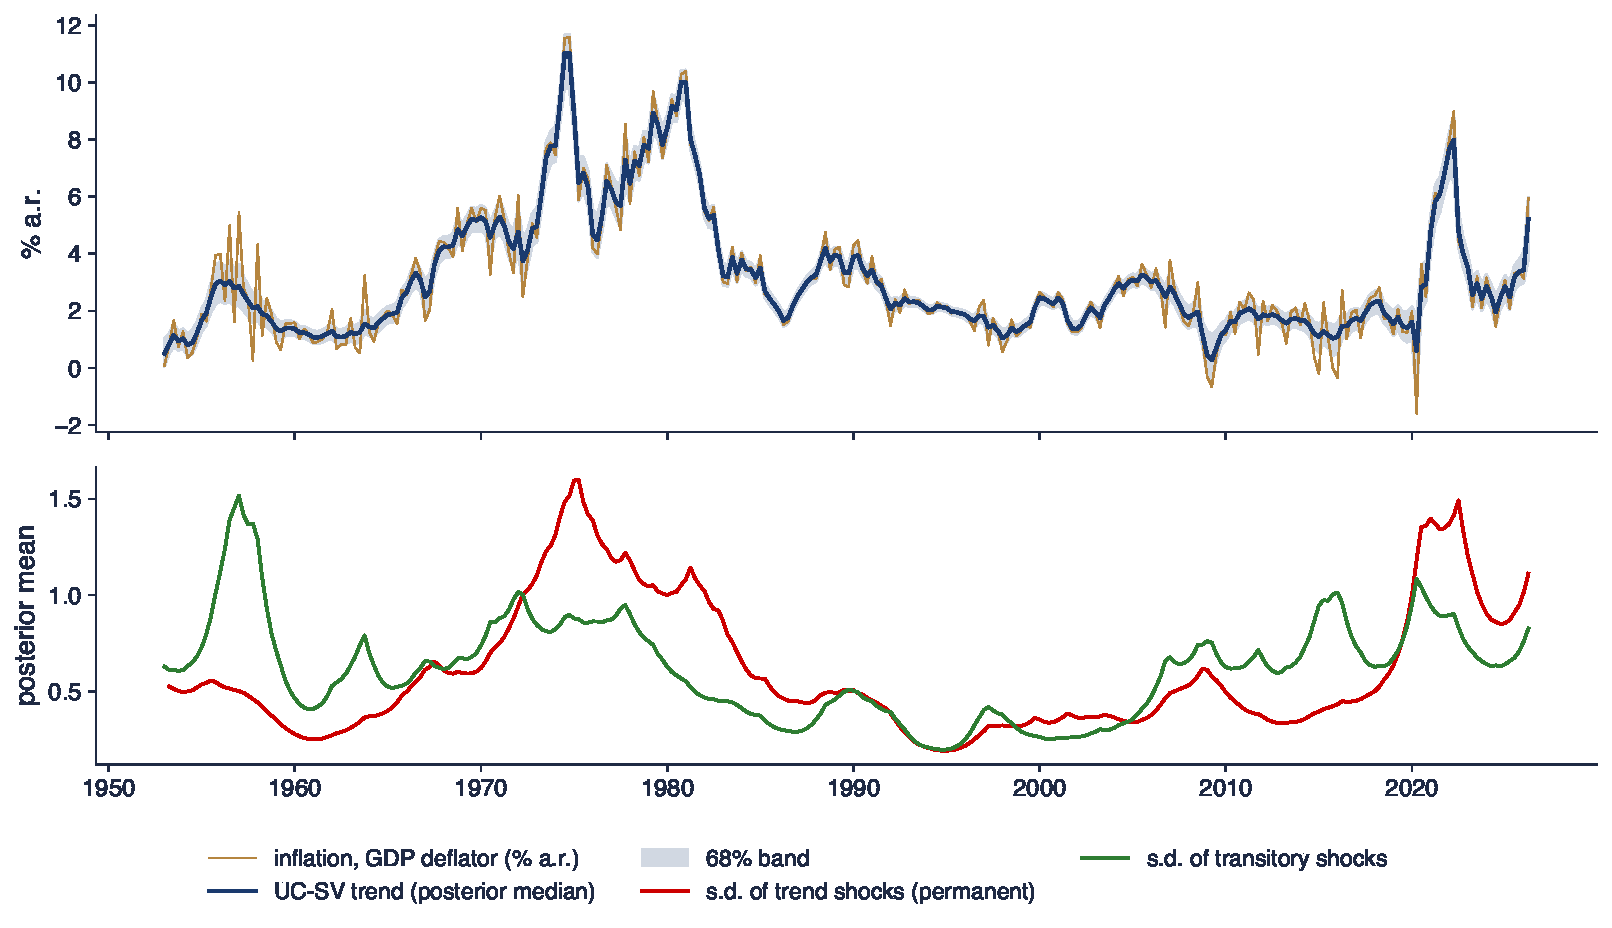
\includegraphics[width=0.97\textwidth,height=0.65\textheight,keepaspectratio]{ats_ch6_ucsv_us.pdf}
\end{center}
\vspace{-0.25cm}
\begin{itemize}
    \item Inflația deflatorului PIB, $T = 294$ trimestre; UC-SV cu $\gamma = 0{,}2$, eșantionator Gibbs; sus: trendul cu bandă de 68\%; jos: mediile a posteriori ale lui $\sigma_{\varepsilon,t}$ (trend) și $\sigma_{\eta,t}$ (tranzitoriu)
\end{itemize}
\quantlet{ATS\_ch6\_ucsv\_inflation}{\qlurl{ATS_ch6_ucsv_inflation}}
\end{frame}

\begin{frame}{Interpretarea inflației de trend din SUA}
\itemsize{\footnotesize}
\begin{itemize}
    \item Trendul: 8{,}9\% în T1 1975, 2{,}1\% în T1 1995, 1{,}4\% în T4 2019, 8{,}0\% [6{,}6; 8{,}9] în T2 2022, 5{,}2\% [3{,}8; 6{,}0] în T2 2026
    \item Șocurile de trend: abaterea standard 1{,}60 în 1975, 0{,}19 în 1995, 1{,}42 în 2022; șocurile tranzitorii: 0{,}88; 0{,}20; 0{,}90
    \item Coeficientul MA implicit $\theta_t$: \ensuremath{-}0{,}20 (1975), \ensuremath{-}0{,}39 (1995), \ensuremath{-}0{,}37 (2019), \ensuremath{-}0{,}24 (2022): inflația a devenit din nou mai apropiată de un mers aleator în 2021--2022
    \item Aceasta este lecția de prognoză din \refSWb: în perioade calme netezim puternic; cînd volatilitatea trendului crește, un model cu coeficienți ficși reacționează prea lent
\end{itemize}
\end{frame}

\begin{frame}{Inflația de trend din România și ținta BNR}
\itemsize{\footnotesize}
\begin{center}
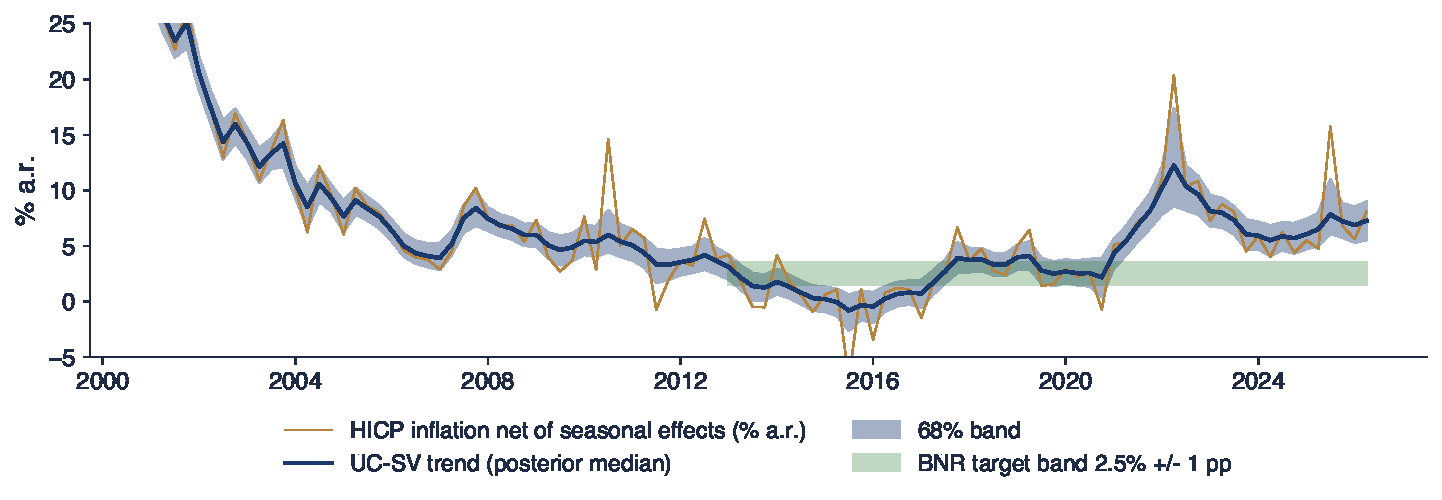
\includegraphics[width=0.97\textwidth,height=0.64\textheight,keepaspectratio]{ats_ch6_ucsv_ro.pdf}
\end{center}
\vspace{-0.25cm}
\begin{itemize}
    \item Inflația IAPC trimestrială (medii trimestriale ale indicelui lunar), $T = 102$, T1 2001--T2 2026; UC-SV cu $\gamma = 0{,}2$ și variabile dummy sezoniere trimestriale; banda-țintă a BNR din 2013
\end{itemize}
\quantlet{ATS\_ch6\_ucsv\_inflation}{\qlurl{ATS_ch6_ucsv_inflation}}
\end{frame}

\begin{frame}{Interpretarea inflației de trend din România}
\itemsize{\small}
\begin{itemize}
    \item Trendul: 8{,}4\% la începutul țintirii inflației (T3 2005), \ensuremath{-}0{,}8\% în T3 2015, 2{,}5\% în T4 2019, 8{,}1\% în T1 2023
    \item Ultimul trimestru: 7{,}3\% [5{,}5; 9{,}0]; probabilitatea a posteriori ca trendul să se afle în intervalul 1,5--3,5\%: 2\%
    \item Din 2013, trendul s-a aflat în bandă doar o parte din timp: sub ea în 2015--2016 (reducerile de TVA), peste ea din 2021
    \item Rezerve: prețurile administrate (plafonările la energie, modificările TVA) intră ca șocuri de trend într-un model univariat; un proiect le poate adăuga ca regresori sau ca o componentă separată
\end{itemize}
\end{frame}

\begin{frame}{Mai departe: BSTS și modele cu schimbare de regim}
\itemsize{\small}
\begin{itemize}
    \item Serii de timp structurale bayesiene \refSV: local linear trend + componentă sezonieră + regresie cu a priori spike-and-slab pe mulți regresori (Google Trends)
    \begin{itemize}
        \item același simulation smoother într-un eșantionator Gibbs; selecția variabilelor pe blocul de regresie
        \item contrafactuali pentru evaluarea politicilor (CausalImpact, \refBro): \atschlink{https://danpele.github.io/Advanced-Time-Series/RO/Cursuri/capitol14_inferenta_cauzala_serii_timp.pdf}{Capitolul 14}
    \end{itemize}
    \item Stări discrete: $s_t \in \{1, \dots, K\}$ cu un lanț Markov; filtrul Hamilton este filtrul Bayes cu sume în loc de integrale
    \begin{itemize}
        \item modele în spațiul stărilor cu schimbare de regim (filtrul Kim, eșantionare Gibbs) \refKN: \atschlink{https://danpele.github.io/Advanced-Time-Series/RO/Cursuri/capitol7_modele_schimbare_regim.pdf}{Capitolul 7}
    \end{itemize}
    \item Evaluarea prognozelor tuturor acestor modele (prognoze de densitate, reguli de scor): \atschlink{https://danpele.github.io/Advanced-Time-Series/RO/Cursuri/capitol1_evaluarea_prognozelor.pdf}{Capitolul 1}
\end{itemize}
\end{frame}

\begin{frame}{Recapitulare: inflația de trend}
\itemsize{\small}
\begin{itemize}
    \item UC-SV permite ca împărțirea dintre șocurile permanente și cele tranzitorii să se schimbe în timp
    \item Două blocuri KSC și o eșantionare pe baza preciziei fac eșantionatorul Gibbs rapid
    \item Inflația de trend din SUA a crescut puternic în 2021--2022; inflația de trend din România este încă peste banda-țintă
\end{itemize}
\end{frame}


%=============================================================================
\section{AI în descoperirea științifică}
%=============================================================================

\begin{frame}{O întrebare deschisă}
\itemsize{\small}
\begin{itemize}
    \item Cît din saltul inflației din 2021--2023 a fost o deplasare a inflației de trend, în SUA și în România, și s-a inversat aceasta?
    \begin{itemize}
        \item formal: distribuția a posteriori a lui $\tau_t$ și a raportului $\sigma_{\varepsilon,t}/\sigma_{\eta,t}$ în UC-SV; infirmată dacă trendul a revenit la nivelul din 2019 cu probabilitate a posteriori mare sub orice specificare preînregistrată
        \item răspunsul univariat depinde de un parametru fixat, $\gamma$: mini studiul de caz de mai jos
    \end{itemize}
    \item Miza: o bancă centrală reacționează diferit la un salt tranzitoriu și la unul persistent; ancorarea este o afirmație despre trend, nu despre inflația totală
    \begin{itemize}
        \item literatura de pornire: \refSWb, \refCSb, \refPri, \refMNZ
    \end{itemize}
\end{itemize}
\end{frame}

\begin{frame}{Bucla de cercetare cu un asistent AI}
\itemsize{\footnotesize}
\begin{itemize}
    \item Un asistent AI (un LLM precum Claude, ChatGPT, Gemini sau Copilot) accelerează fiecare etapă; Semantic Scholar și Elicit ajută la literatură
    \begin{itemize}
        \item \textbf{literatura}: \aiprompt{Listează lucrări recenzate care estimează inflația de trend cu volatilitate stochastică pentru țări europene după 2021; dă DOI-urile.} Apoi verificați fiecare DOI pe Crossref
        \item \textbf{ipoteza}: \aiprompt{Propune trei implicații observabile care deosebesc o deplasare a trendului de o succesiune de șocuri tranzitorii mari.}
        \item \textbf{cod și replicare}: cereți un eșantionator Gibbs pentru UC-SV, apoi reproduceți întîi o cifră cunoscută (trendul pentru SUA din acest curs)
        \item \textbf{robustețe și critică}: \aiprompt{Joacă rolul unui recenzent ostil: ce alegeri fixate ale unui model UC-SV ar putea schimba concluzia despre 2022?}
    \end{itemize}
    \item Raportul: ce s-a cerut, ce s-a păstrat, ce s-a respins (AI\_USE.md, AI\_ERRORS.md)
\end{itemize}
\end{frame}

\begin{frame}{Verificări necesare}
\itemsize{\small}
\begin{itemize}
    \item Fiecare referință există și spune ce se afirmă (DOI-ul funcționează, titlul coincide, rezultatul se află în lucrare)
    \item Eșantionatorul are ca țintă distribuția a posteriori declarată: testați-l pe un model cu răspuns cunoscut (netezitorul Kalman, ca în verificarea celor trei eșantionatoare)
    \item Convergența este raportată: mai multe lanțuri, factori de ineficiență, efectul dublării numărului de extrageri
    \item Alegerile fixate ($\gamma$, constanta KSC, distribuțiile a priori, tratarea sezonalității, data de început) sînt enumerate și variate înaintea concluziilor
    \item Estimațiile de la finalul eșantionului sînt raportate ca valori filtrate, cu benzile lor, nu ca estimații punctuale netezite
\end{itemize}
\end{frame}

\begin{frame}{Mini studiu de caz: un parametru fixat, patru trenduri}
\itemsize{\footnotesize}
\begin{center}
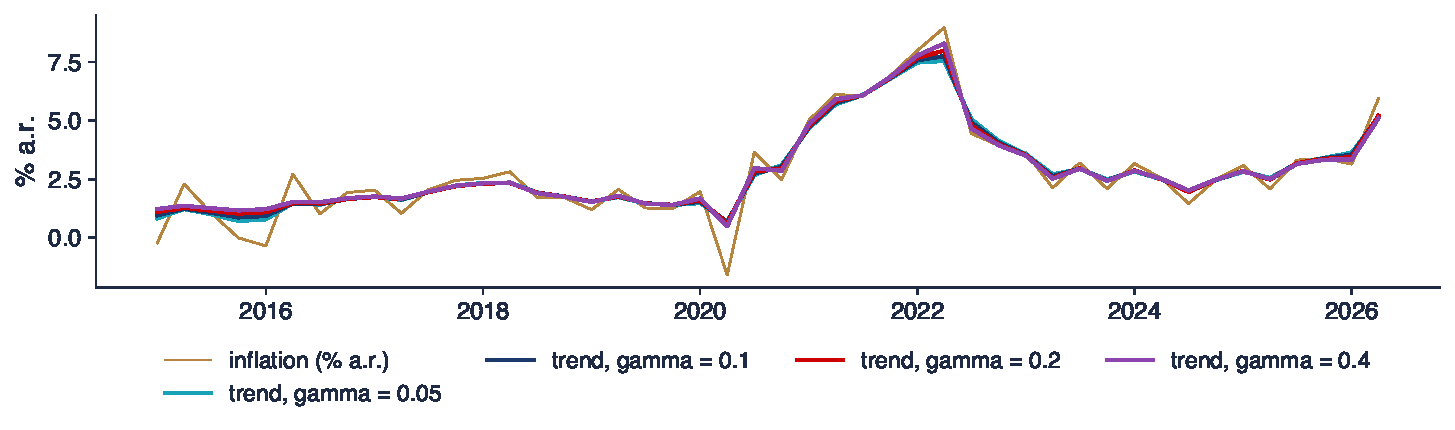
\includegraphics[width=0.97\textwidth,height=0.55\textheight,keepaspectratio]{ats_ch6_ai_case.pdf}
\end{center}
\vspace{-0.25cm}
\begin{itemize}
    \item Trendul UC-SV pentru SUA din 2015, pentru $\gamma \in \{0{,}05; 0{,}1; 0{,}2; 0{,}4\}$: trendul în T2 2022 7{,}6; 7{,}8; 8{,}0; 8{,}3\% (inflația 9{,}0\%); în ultimul trimestru 5{,}1; 5{,}2; 5{,}2; 5{,}1\%
    \item Ordinea este stabilă, dar nivelul trendului din 2022 nu este: un rezumat AI care raportează „inflația de trend a atins un maxim de X\%” fără $\gamma$ ascunde o alegere de modelare
\end{itemize}
\quantlet{ATS\_ch6\_ai\_robustness}{\qlurl{ATS_ch6_ai_robustness}}
\end{frame}

\begin{frame}{Idee de proiect}
\itemsize{\small}
\begin{itemize}
    \item \textbf{Inflația de trend și ancorarea în Europa Centrală și de Est}: întîi replicare, apoi extindere
    \begin{itemize}
        \item replicați: trendul UC-SV pentru SUA din acest curs (T2 2022: 8{,}0\%) și trendul pentru România (7{,}3\% în T2 2026)
        \item extindeți: România, Ungaria, Polonia și Cehia; un UC-SV multivariat cu un trend comun al zonei euro; prețurile administrate ca o componentă separată; $\gamma$ estimat cu o distribuție a priori în loc să fie fixat
        \item preînregistrați: datele, eșantionul, distribuțiile a priori, statistica de ancorare (probabilitatea a posteriori de a fi în banda-țintă), exercițiul în timp real și grila de robustețe
    \end{itemize}
    \item Livrabilele urmează regulile cursului: repository, raport, AI\_USE.md, AI\_ERRORS.md, susținere orală
\end{itemize}
\end{frame}


%=============================================================================
\section{Încheiere}
%=============================================================================

\begin{frame}{Idei de reținut}
\itemsize{\small}
\begin{itemize}
    \item Filtrul Kalman este condiționarea gaussiană aplicată recursiv; netezitorul, verosimilitatea și simulation smoother-ul decurg din ea
    \item Inițializați exact stările nestaționare; tratați varianțele nule ca probleme de frontieră
    \item Spațiul stărilor bayesian: eșantionați traiectorii întregi; FFBS, DK și eșantionarea pe baza preciziei sînt interschimbabile
    \item Volatilitatea stochastică nu este GARCH; mixtura KSC și filtrele de particule o fac tratabilă
    \item Mărimile latente (output gap-uri, trenduri, pante variabile în timp) au o incertitudine care depinde de model: raportați benzi, valori filtrate și alternative
\end{itemize}
\end{frame}

\begin{frame}{Autoevaluare}
\itemsize{\small}
\begin{columns}[T]
\begin{column}{0.58\textwidth}
\begin{block}{Întrebări}
\begin{itemize}
    \item De ce scade nelimitat log-verosimilitatea big kappa cînd $\kappa$ crește?
    \item Ce vă spune o estimație ML $\hat\sigma^2_\eta = 0$ despre un model local level?
    \item De ce are nevoie simulation smoother-ul DK doar de netezitorul mediei?
    \item De ce este zero cîștigul EKF în modelul SV?
    \item De ce este $\ln\hat L$ deplasat, deși $\hat L$ este nedeplasat?
    \item Ce restricție face ca ciclul UC să difere de ciclul BN?
\end{itemize}
\end{block}
\end{column}
\begin{column}{0.38\textwidth}
\begin{block}{Urmează: \atschlink{https://danpele.github.io/Advanced-Time-Series/RO/Cursuri/capitol7_modele_schimbare_regim.pdf}{Capitolul 7}}
\begin{itemize}
    \item Modele cu schimbare de regim
    \item Stări ascunse discrete: filtrul Hamilton, netezitorul Kim, EM și Gibbs pentru modelele Markov switching și modele în spațiul stărilor cu regimuri
\end{itemize}
\end{block}
\end{column}
\end{columns}
\end{frame}


%=============================================================================
\section{Anexă}
%=============================================================================

\begin{frame}{Anexă: filtrul Kalman din lemă}
\hypertarget{atsapp1}{}\atsappback{atssrc1}{Înapoi}
\itemsize{\small}
\begin{itemize}
    \item Dat $Y_{t-1}$: $\begin{pmatrix}\alpha_t\\ y_t\end{pmatrix} \sim N\left(\begin{pmatrix}a_t\\ Z_ta_t\end{pmatrix}, \begin{pmatrix}P_t & P_tZ_t'\\ Z_tP_t & F_t\end{pmatrix}\right)$, $F_t = Z_tP_tZ_t' + H_t$
    \item Condiționarea pe $y_t$ (echivalent pe $v_t$, deoarece $Y_t = (Y_{t-1}, v_t)$, iar $v_t$ este independent de $Y_{t-1}$) dă $a_{t|t}$ și $P_{t|t}$
    \item $\alpha_{t+1} = c_t + T_t\alpha_t + R_t\eta_t$ cu $\eta_t$ independent de $Y_t$: $a_{t+1} = c_t + T_ta_{t|t}$, $P_{t+1} = T_tP_{t|t}T_t' + R_tQ_tR_t'$
    \item Netezitorul: $\hat\alpha_t = a_t + \sum_{j=t}^n\Cov(\alpha_t, v_j)F_j^{-1}v_j$ (variabilele $v_j$ sînt independente); $\Cov(\alpha_t, v_j) = P_tL_t'\cdots L_{j-1}'Z_j'$ dă $\hat\alpha_t = a_t + P_tr_{t-1}$
\end{itemize}
\end{frame}

\begin{frame}{Anexă: exactitatea simulation smoother-ului Durbin--Koopman}
\hypertarget{atsapp2}{}\atsappback{atssrc2}{Înapoi}
\itemsize{\small}
\begin{itemize}
    \item Modelul gaussian: $\alpha | y \sim N(\hat\alpha(y), V)$, cu $V$ independent de $y$, iar $\hat\alpha(y)$ liniar în $y$ (afin, cu termenii liberi)
    \item Pentru o extragere $(\alpha^+, y^+)$ din legea comună, $\alpha^+ - \hat\alpha(y^+) \sim N(0, V)$ și este independentă de $y^+$ (și de $y$)
    \item Deci $\tilde\alpha = \hat\alpha(y) + \alpha^+ - \hat\alpha(y^+) \sim N(\hat\alpha(y), V)$; liniaritatea dă $\hat\alpha(y) - \hat\alpha(y^+) = \hat\alpha_0(y - y^+)$, o singură trecere a netezitorului cu termeni liberi nuli
    \item Stările difuze: netezitorul difuz exact este invariant la partea difuză a lui $\alpha_1^+$, deci aceasta poate fi fixată la $a_1$
\end{itemize}
\end{frame}

\begin{frame}{Anexă: nedeplasarea verosimilității din filtrul de particule}
\hypertarget{atsapp3}{}\atsappback{atssrc3}{Înapoi}
\itemsize{\small}
\begin{itemize}
    \item Filtrul bootstrap, un pas: $\E[\frac1N\sum_iw^{(i)}_t\,|\,\mathcal F_{t-1}] = \int g(y_t | x)\,\hat p_{N}(x | Y_{t-1})\,dx$, unde $\hat p_N$ este legea predictivă empirică a particulelor
    \item Aplicînd succesiv proprietatea speranțelor condiționate iterate pentru $t = n, n-1, \dots, 1$ (la fiecare pas, speranța ultimului factor condiționată de $\mathcal F_{t-1}$ se înlocuiește cu formula de mai sus), cu reeșantionare multinomială sau sistematică, obținem $\E\prod_t\hat p(y_t | Y_{t-1}) = p(y_{1:n})$ \refDM
    \item Fiecare factor este o estimație de tip raport, dar produsul este nedeplasat, pentru că reeșantionarea păstrează ponderile așteptate; mărimile normalizate (mediile filtrate) sînt doar consistente
    \item Jensen: $\E\ln\hat L \le \ln\E\hat L = \ln L$; sub o TLC pentru $\ln\hat L$, deplasarea este $-\frac12\Var(\ln\hat L)$
\end{itemize}
\end{frame}


%=============================================================================
\section{Bibliografie}
%=============================================================================

\begin{frame}{Bibliografie (1/5)}
\itemsize{\tiny}
\begin{itemize}
    \item Aguiar, M., \& Gopinath, G. (2007). Emerging market business cycles: The cycle is the trend. \textit{Journal of Political Economy}, 115(1), 69--102. \href{https://doi.org/10.1086/511283}{doi:10.1086/511283}
    \item Andrieu, C., Doucet, A., \& Holenstein, R. (2010). Particle Markov chain Monte Carlo methods. \textit{Journal of the Royal Statistical Society: Series B}, 72(3), 269--342. \href{https://doi.org/10.1111/j.1467-9868.2009.00736.x}{doi:10.1111/j.1467-9868.2009.00736.x}
    \item Andrieu, C., \& Roberts, G. O. (2009). The pseudo-marginal approach for efficient Monte Carlo computations. \textit{The Annals of Statistics}, 37(2), 697--725. \href{https://doi.org/10.1214/07-AOS574}{doi:10.1214/07-AOS574}
    \item Ansley, C. F., \& Kohn, R. (1985). Estimation, filtering, and smoothing in state space models with incompletely specified initial conditions. \textit{The Annals of Statistics}, 13(4), 1286--1316. \href{https://doi.org/10.1214/aos/1176349739}{doi:10.1214/aos/1176349739}
    \item Bańbura, M., \& Modugno, M. (2014). Maximum likelihood estimation of factor models on datasets with arbitrary pattern of missing data. \textit{Journal of Applied Econometrics}, 29(1), 133--160. \href{https://doi.org/10.1002/jae.2306}{doi:10.1002/jae.2306}
    \item Beveridge, S., \& Nelson, C. R. (1981). A new approach to decomposition of economic time series into permanent and transitory components with particular attention to measurement of the `business cycle'. \textit{Journal of Monetary Economics}, 7(2), 151--174. \href{https://doi.org/10.1016/0304-3932(81)90040-4}{doi:10.1016/0304-3932(81)90040-4}
    \item Bollerslev, T. (1986). Generalized autoregressive conditional heteroskedasticity. \textit{Journal of Econometrics}, 31(3), 307--327. \href{https://doi.org/10.1016/0304-4076(86)90063-1}{doi:10.1016/0304-4076(86)90063-1}
    \item Brodersen, K. H., Gallusser, F., Koehler, J., Remy, N., \& Scott, S. L. (2015). Inferring causal impact using Bayesian structural time-series models. \textit{The Annals of Applied Statistics}, 9(1), 247--274. \href{https://doi.org/10.1214/14-AOAS788}{doi:10.1214/14-AOAS788}
    \item Carter, C. K., \& Kohn, R. (1994). On Gibbs sampling for state space models. \textit{Biometrika}, 81(3), 541--553. \href{https://doi.org/10.1093/biomet/81.3.541}{doi:10.1093/biomet/81.3.541}
    \item Chan, J. C. C., \& Jeliazkov, I. (2009). Efficient simulation and integrated likelihood estimation in state space models. \textit{International Journal of Mathematical Modelling and Numerical Optimisation}, 1(1/2), 101--120. \href{https://doi.org/10.1504/IJMMNO.2009.030090}{doi:10.1504/IJMMNO.2009.030090}
    \item Chopin, N., \& Papaspiliopoulos, O. (2020). \textit{An Introduction to Sequential Monte Carlo}. Springer. \href{https://doi.org/10.1007/978-3-030-47845-2}{doi:10.1007/978-3-030-47845-2}
    \item Clark, P. K. (1987). The cyclical component of U.S. economic activity. \textit{The Quarterly Journal of Economics}, 102(4), 797--814. \href{https://doi.org/10.2307/1884282}{doi:10.2307/1884282}
\end{itemize}
\end{frame}

\begin{frame}{Bibliografie (2/5)}
\itemsize{\tiny}
\begin{itemize}
    \item Cogley, T., \& Sargent, T. J. (2001). Evolving post-World War II U.S. inflation dynamics. \textit{NBER Macroeconomics Annual}, 16, 331--373. \href{https://doi.org/10.1086/654451}{doi:10.1086/654451}
    \item Cogley, T., \& Sargent, T. J. (2005). Drifts and volatilities: Monetary policies and outcomes in the post WWII US. \textit{Review of Economic Dynamics}, 8(2), 262--302. \href{https://doi.org/10.1016/j.red.2004.10.009}{doi:10.1016/j.red.2004.10.009}
    \item de Jong, P. (1991). The diffuse Kalman filter. \textit{The Annals of Statistics}, 19(2), 1073--1083. \href{https://doi.org/10.1214/aos/1176348139}{doi:10.1214/aos/1176348139}
    \item de Jong, P., \& Shephard, N. (1995). The simulation smoother for time series models. \textit{Biometrika}, 82(2), 339--350. \href{https://doi.org/10.1093/biomet/82.2.339}{doi:10.1093/biomet/82.2.339}
    \item Del Moral, P. (2004). \textit{Feynman--Kac Formulae: Genealogical and Interacting Particle Systems with Applications}. Springer. \href{https://doi.org/10.1007/978-1-4684-9393-1}{doi:10.1007/978-1-4684-9393-1}
    \item Del Negro, M., \& Primiceri, G. E. (2015). Time varying structural vector autoregressions and monetary policy: A corrigendum. \textit{The Review of Economic Studies}, 82(4), 1342--1345. \href{https://doi.org/10.1093/restud/rdv024}{doi:10.1093/restud/rdv024}
    \item Doucet, A., Pitt, M. K., Deligiannidis, G., \& Kohn, R. (2015). Efficient implementation of Markov chain Monte Carlo when using an unbiased likelihood estimator. \textit{Biometrika}, 102(2), 295--313. \href{https://doi.org/10.1093/biomet/asu075}{doi:10.1093/biomet/asu075}
    \item Doz, C., Giannone, D., \& Reichlin, L. (2011). A two-step estimator for large approximate dynamic factor models based on Kalman filtering. \textit{Journal of Econometrics}, 164(1), 188--205. \href{https://doi.org/10.1016/j.jeconom.2011.02.012}{doi:10.1016/j.jeconom.2011.02.012}
    \item Durbin, J., \& Koopman, S. J. (2002). A simple and efficient simulation smoother for state space time series analysis. \textit{Biometrika}, 89(3), 603--616. \href{https://doi.org/10.1093/biomet/89.3.603}{doi:10.1093/biomet/89.3.603}
    \item Durbin, J., \& Koopman, S. J. (2012). \textit{Time Series Analysis by State Space Methods} (2nd ed.). Oxford University Press. \href{https://doi.org/10.1093/acprof:oso/9780199641178.001.0001}{doi:10.1093/acprof:oso/9780199641178.001.0001}
    \item Frühwirth-Schnatter, S. (1994). Data augmentation and dynamic linear models. \textit{Journal of Time Series Analysis}, 15(2), 183--202. \href{https://doi.org/10.1111/j.1467-9892.1994.tb00184.x}{doi:10.1111/j.1467-9892.1994.tb00184.x}
    \item Frühwirth-Schnatter, S., \& Wagner, H. (2010). Stochastic model specification search for Gaussian and partial non-Gaussian state space models. \textit{Journal of Econometrics}, 154(1), 85--100. \href{https://doi.org/10.1016/j.jeconom.2009.07.003}{doi:10.1016/j.jeconom.2009.07.003}
\end{itemize}
\end{frame}

\begin{frame}{Bibliografie (3/5)}
\itemsize{\tiny}
\begin{itemize}
    \item Giannone, D., Reichlin, L., \& Small, D. (2008). Nowcasting: The real-time informational content of macroeconomic data. \textit{Journal of Monetary Economics}, 55(4), 665--676. \href{https://doi.org/10.1016/j.jmoneco.2008.05.010}{doi:10.1016/j.jmoneco.2008.05.010}
    \item Gordon, N. J., Salmond, D. J., \& Smith, A. F. M. (1993). Novel approach to nonlinear/non-Gaussian Bayesian state estimation. \textit{IEE Proceedings F (Radar and Signal Processing)}, 140(2), 107--113. \href{https://doi.org/10.1049/ip-f-2.1993.0015}{doi:10.1049/ip-f-2.1993.0015}
    \item Hamilton, J. D. (1994). \textit{Time Series Analysis}. Princeton University Press. \href{https://doi.org/10.2307/j.ctv14jx6sm}{doi:10.2307/j.ctv14jx6sm}
    \item Hamilton, J. D. (2018). Why you should never use the Hodrick--Prescott filter. \textit{The Review of Economics and Statistics}, 100(5), 831--843. \href{https://doi.org/10.1162/rest_a_00706}{doi:10.1162/rest\_a\_00706}
    \item Harvey, A. C. (1990). \textit{Forecasting, Structural Time Series Models and the Kalman Filter}. Cambridge University Press. \href{https://doi.org/10.1017/CBO9781107049994}{doi:10.1017/CBO9781107049994}
    \item Harvey, A. C., \& Jaeger, A. (1993). Detrending, stylized facts and the business cycle. \textit{Journal of Applied Econometrics}, 8(3), 231--247. \href{https://doi.org/10.1002/jae.3950080302}{doi:10.1002/jae.3950080302}
    \item Harvey, A., Ruiz, E., \& Shephard, N. (1994). Multivariate stochastic variance models. \textit{The Review of Economic Studies}, 61(2), 247--264. \href{https://doi.org/10.2307/2297980}{doi:10.2307/2297980}
    \item Jacquier, E., Polson, N. G., \& Rossi, P. E. (1994). Bayesian analysis of stochastic volatility models. \textit{Journal of Business \& Economic Statistics}, 12(4), 371--389. \href{https://doi.org/10.1080/07350015.1994.10524553}{doi:10.1080/07350015.1994.10524553}
    \item Julier, S. J., \& Uhlmann, J. K. (2004). Unscented filtering and nonlinear estimation. \textit{Proceedings of the IEEE}, 92(3), 401--422. \href{https://doi.org/10.1109/JPROC.2003.823141}{doi:10.1109/JPROC.2003.823141}
    \item Jungbacker, B., \& Koopman, S. J. (2015). Likelihood-based dynamic factor analysis for measurement and forecasting. \textit{The Econometrics Journal}, 18(2), C1--C21. \href{https://doi.org/10.1111/ectj.12029}{doi:10.1111/ectj.12029}
    \item Kalman, R. E. (1960). A new approach to linear filtering and prediction problems. \textit{Journal of Basic Engineering}, 82(1), 35--45. \href{https://doi.org/10.1115/1.3662552}{doi:10.1115/1.3662552}
    \item Kamber, G., Morley, J., \& Wong, B. (2018). Intuitive and reliable estimates of the output gap from a Beveridge--Nelson filter. \textit{The Review of Economics and Statistics}, 100(3), 550--566. \href{https://doi.org/10.1162/REST_a_00691}{doi:10.1162/REST\_a\_00691}
\end{itemize}
\end{frame}

\begin{frame}{Bibliografie (4/5)}
\itemsize{\tiny}
\begin{itemize}
    \item Kim, C.-J., \& Nelson, C. R. (1999). \textit{State-Space Models with Regime Switching: Classical and Gibbs-Sampling Approaches with Applications}. MIT Press. \href{https://doi.org/10.7551/mitpress/6444.001.0001}{doi:10.7551/mitpress/6444.001.0001}
    \item Kim, S., Shephard, N., \& Chib, S. (1998). Stochastic volatility: Likelihood inference and comparison with ARCH models. \textit{The Review of Economic Studies}, 65(3), 361--393. \href{https://doi.org/10.1111/1467-937X.00050}{doi:10.1111/1467-937X.00050}
    \item Kitagawa, G. (1996). Monte Carlo filter and smoother for non-Gaussian nonlinear state space models. \textit{Journal of Computational and Graphical Statistics}, 5(1), 1--25. \href{https://doi.org/10.1080/10618600.1996.10474692}{doi:10.1080/10618600.1996.10474692}
    \item Koopman, S. J. (1997). Exact initial Kalman filtering and smoothing for nonstationary time series models. \textit{Journal of the American Statistical Association}, 92(440), 1630--1638. \href{https://doi.org/10.1080/01621459.1997.10473685}{doi:10.1080/01621459.1997.10473685}
    \item Koopman, S. J., \& Durbin, J. (2000). Fast filtering and smoothing for multivariate state space models. \textit{Journal of Time Series Analysis}, 21(3), 281--296. \href{https://doi.org/10.1111/1467-9892.00186}{doi:10.1111/1467-9892.00186}
    \item Mariano, R. S., \& Murasawa, Y. (2003). A new coincident index of business cycles based on monthly and quarterly series. \textit{Journal of Applied Econometrics}, 18(4), 427--443. \href{https://doi.org/10.1002/jae.695}{doi:10.1002/jae.695}
    \item Morley, J. C., Nelson, C. R., \& Zivot, E. (2003). Why are the Beveridge--Nelson and unobserved-components decompositions of GDP so different? \textit{The Review of Economics and Statistics}, 85(2), 235--243. \href{https://doi.org/10.1162/003465303765299765}{doi:10.1162/003465303765299765}
    \item Omori, Y., Chib, S., Shephard, N., \& Nakajima, J. (2007). Stochastic volatility with leverage: Fast and efficient likelihood inference. \textit{Journal of Econometrics}, 140(2), 425--449. \href{https://doi.org/10.1016/j.jeconom.2006.07.008}{doi:10.1016/j.jeconom.2006.07.008}
    \item Orphanides, A., \& van Norden, S. (2002). The unreliability of output-gap estimates in real time. \textit{The Review of Economics and Statistics}, 84(4), 569--583. \href{https://doi.org/10.1162/003465302760556422}{doi:10.1162/003465302760556422}
    \item Petropoulos, F., Apiletti, D., Assimakopoulos, V., Babai, M. Z., et al.\ (2022). Forecasting: Theory and practice. \textit{International Journal of Forecasting}, 38(3), 705--871. \href{https://doi.org/10.1016/j.ijforecast.2021.11.001}{doi:10.1016/j.ijforecast.2021.11.001}
    \item Pitt, M. K., \& Shephard, N. (1999). Filtering via simulation: Auxiliary particle filters. \textit{Journal of the American Statistical Association}, 94(446), 590--599. \href{https://doi.org/10.1080/01621459.1999.10474153}{doi:10.1080/01621459.1999.10474153}
    \item Pitt, M. K., Silva, R. d. S., Giordani, P., \& Kohn, R. (2012). On some properties of Markov chain Monte Carlo simulation methods based on the particle filter. \textit{Journal of Econometrics}, 171(2), 134--151. \href{https://doi.org/10.1016/j.jeconom.2012.06.004}{doi:10.1016/j.jeconom.2012.06.004}
\end{itemize}
\end{frame}

\begin{frame}{Bibliografie (5/5)}
\itemsize{\tiny}
\begin{itemize}
    \item Primiceri, G. E. (2005). Time varying structural vector autoregressions and monetary policy. \textit{The Review of Economic Studies}, 72(3), 821--852. \href{https://doi.org/10.1111/j.1467-937X.2005.00353.x}{doi:10.1111/j.1467-937X.2005.00353.x}
    \item Scott, S. L., \& Varian, H. R. (2014). Predicting the present with Bayesian structural time series. \textit{International Journal of Mathematical Modelling and Numerical Optimisation}, 5(1/2), 4--23. \href{https://doi.org/10.1504/IJMMNO.2014.059942}{doi:10.1504/IJMMNO.2014.059942}
    \item Shephard, N., \& Harvey, A. C. (1990). On the probability of estimating a deterministic component in the local level model. \textit{Journal of Time Series Analysis}, 11(4), 339--347. \href{https://doi.org/10.1111/j.1467-9892.1990.tb00062.x}{doi:10.1111/j.1467-9892.1990.tb00062.x}
    \item Shumway, R. H., \& Stoffer, D. S. (1982). An approach to time series smoothing and forecasting using the EM algorithm. \textit{Journal of Time Series Analysis}, 3(4), 253--264. \href{https://doi.org/10.1111/j.1467-9892.1982.tb00349.x}{doi:10.1111/j.1467-9892.1982.tb00349.x}
    \item Stock, J. H., \& Watson, M. W. (1998). Median unbiased estimation of coefficient variance in a time-varying parameter model. \textit{Journal of the American Statistical Association}, 93(441), 349--358. \href{https://doi.org/10.1080/01621459.1998.10474116}{doi:10.1080/01621459.1998.10474116}
    \item Stock, J. H., \& Watson, M. W. (2007). Why has U.S. inflation become harder to forecast? \textit{Journal of Money, Credit and Banking}, 39(s1), 3--33. \href{https://doi.org/10.1111/j.1538-4616.2007.00014.x}{doi:10.1111/j.1538-4616.2007.00014.x}
    \item Taylor, S. J. (1994). Modeling stochastic volatility: A review and comparative study. \textit{Mathematical Finance}, 4(2), 183--204. \href{https://doi.org/10.1111/j.1467-9965.1994.tb00057.x}{doi:10.1111/j.1467-9965.1994.tb00057.x}
    \item Watson, M. W. (1986). Univariate detrending methods with stochastic trends. \textit{Journal of Monetary Economics}, 18(1), 49--75. \href{https://doi.org/10.1016/0304-3932(86)90054-1}{doi:10.1016/0304-3932(86)90054-1}
\end{itemize}
\end{frame}

\end{document}
